\documentclass[options]{mwart}

\usepackage{polski}
\usepackage[utf8]{inputenc}

\usepackage{amsthm}
\usepackage{amsmath}
\usepackage{amssymb}

\usepackage{mdframed}
\usepackage{hyperref}
\usepackage{graphicx}  
\usepackage{url}
\usepackage{enumitem}


\usepackage{caption}    % Do podpisów pod obrazami
\usepackage{float}      % Do precyzyjnego umiejscowienia obrazów



\usepackage{fancyhdr}
\pagestyle{fancy}
\fancyhf{}

\fancyhead[L]{
\includegraphics[height=0.666cm]{logo_projektu.png}}
\fancyhead[C]{\textit{Projekt poprawy jakości zdjęć}}
\fancyhead[R]{
\includegraphics[height=0.666cm]{logo_uczelni.png}}
\fancyfoot[C]{\thepage}

\setlength{\headheight}{20pt}  % Możesz dostosować wartość np. 20pt



\usepackage{listings}
\usepackage{xcolor} % Kolory dla kodu

\lstset{
    language=Matlab, % Można zmienić na inny język np. C, Java, bash
    basicstyle=\ttfamily\small, % Czcionka kodu
    keywordstyle=\color{blue}, % Słowa kluczowe
    commentstyle=\color{gray}, % Komentarze
    stringstyle=\color{red}, % Ciągi znaków
    numbers=left, % Numerowanie linii
    numberstyle=\tiny\color{gray}, % Styl numerów
    stepnumber=1, % Co ile numerować
    frame=single, % Ramka wokół kodu
    breaklines=true, % Zawijanie linii
    tabsize=3 % Rozmiar tabulatora
}






\begin{document}
\thispagestyle{empty}

\begin{figure}[h]
    \centering
    
\includegraphics[width=1\textwidth]{logo_uczelni.png}
\end{figure}

%    \title{Projekt poprawy jakości zdjęć \\ \large{Raport 1}}
%    \date{\today}
%    %\author{\textit{Pod opieką: prof. dr hab. inż. Artura Przylaskowskiego}}
%    \maketitle
%    \begin{center}
%        \textit{Pod opieką: prof. dr hab. inż. Artura Przylaskowskiego}
%    \end{center}

\begin{center}
    {\LARGE \textbf{Projekt poprawy jakości zdjęć analogowych i cyfrowych o skrajnej jasności}} \\[0.3cm]
    {\large \textbf{Raport I}} \\[0.2cm]
    \textit{projekt realizowany pod opieką prof. dr hab. inż. Artura Przelaskowskiego}

\end{center}

\begin{figure}[h]
    \centering
    
\includegraphics[width=1\textwidth]{logo_projektu.png}
\end{figure}

\vfill
\begin{abstract}
    Raport 1 projektu poprawy jakości zdjęć wykonanych analogowych przez grupę wtorkową z godziny 18
    w składzie:  Bartosz Wójcik, Katarzyna Szwed, Natalia Szymańska,
    Patrycja Szałajko, Aleksandra Wójcik, Karol Sęk, Michał Juszkiewicz, Filip Sajko.

    W tym raporcie skupimy się na opisie procesu wyboru tematu projektu, jego definiowaniu
    i planach jego analizy i rozwiązania. Ponadto wykonamy zdjęcia i zaczniemy je analizować.
\end{abstract}

\newpage
\tableofcontents{}

\newpage



\section{Wstęp}
\subsection{Wybór problemu}
Podczas wyboru tematu projektu kierowaliśmy się użytecznością
i ponadczasowością naszej pracy oraz tym, żeby nasz program
rozwiązywał problem,  który zauważamy na co dzień. Zebraliśmy
kilka naszych najlepszych pomysłów.

Były to: silnik szachowy, inteligentne
rekomendacje muzyki, wydobywanie detali ze zdjęć o ekstremalnej
jasności, opracowywanie wykresów związków chemicznych.
Dodatkowo przeprowadziliśmy ankietę wśród wybranych 27
studentów naszej uczelni. Zapytaliśmy ich, rozwiązanie
którego z powyższych problemów chcieliby zobaczyć.
Wyniki ankiety przedstawiamy poniżej:

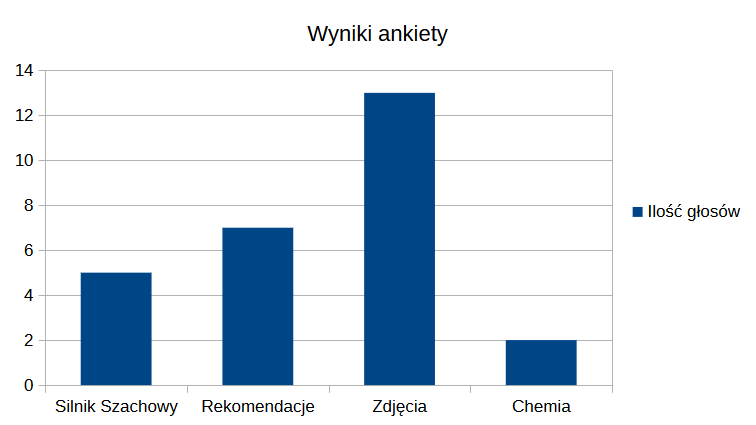
\includegraphics[width=1\textwidth]{wyniki_ankiety.png}

Jak widać zdecydowanie największą popularnością
cieszył się pomysł stworzenia programu poprawiającego jakość zdjęć.

\subsection{Cel projektu}
W ramach tego projektu skoncentrujemy się na opracowaniu metod
umożliwiających stworzenie algorytmu, który normalizuje jasność
zdjęć charakteryzujących się niedoświetleniem lub
prześwietleniem. Na podstawie tego algorytmu planujemy opracować
przyjazną użytkownikowi aplikację, dedykowaną poprawie jakości
amatorskich fotografii. Odbiorcami naszego projektu są zarówno
miłośnicy fotografii analogowej, jak i entuzjaści, którzy nie
dysponują zaawansowanym sprzętem fotograficznym, a także
wszyscy ci, którzy chcą wydobyć z archiwów rodzinnych
nową jakość.

Fotografia analogowa, w przeciwieństwie do fotografii cyfrowej,
nie pozwala na weryfikację efektów pracy tuż po wykonaniu zdjęcia.
O błędach technicznych fotograf dowiaduje się dopiero po wywołaniu
kliszy, co nie pozwala na wprowadzanie poprawek na bieżąco.
Kluczowym aspektem wykonania poprawnej fotografii jest odpowiednie
naświetlenie zdjęcia -- aby uniknąć utraty detali w światłach i cieniach.

Naszym celem jest poprawianie jakości i wyciąganie szczegółów
z zdjęć, w których te szczegóły zostały ukryte i utracone w wyniku
niedoświetlenia i prześwietlenia.

\subsection{Wykorzystywane materiały}
Badania będziemy przeprowadzać z wykorzystaniem zdjęć zrobionych
zarówno przy użyciu aparatu analogowego, jak i cyfrowego. Problemy,
które dotykają fotografii analogowej łatwo powtórzyć na aparacie cyfrowym
ustawiając korektę ekspozycji.
Celowo zrobimy zdjęcia jednego ujęcia o różnym poziomie naświetlenia tak,
abyśmy mogli na nich testować algorytm wiedząc, jakich wyników powinniśmy
się spodziewać. Dodatkowo zależy nam na pozyskaniu informacji w jaki sposób zdjęcia doświetlone niepoprawnie odstają od poprawnej ekspozycji.
Zależy nam, aby zdjęcia były o różnorodnej tematyce -- od zdjęć
natury przez portrety po zdjęcia architektury tak, aby mieć pewność, że nasza
metoda ma szerokie zastosowanie w życiu codziennym.


\subsection{Dobór zdjęć}
Będziemy pracować na wysokiej jakości cyfrowych skanach filmu zdjęć
analogowych, a także na typowych dla nas cyfrowych zdjęciach.
Posłużymy się archiwalnymi zdjęciami znalezionymi w
rodzinnych albumach, naszych własnych kolekcjach i wykonanymi
celowo na potrzeby tego projektu.

W tym celu kilkoro członków naszego zespołu chwyciło
za aparaty, i ruszyło fotografować świat!

\newpage
\section{Zdjęcia!}
Kilka przykładowych zdjęć spośród zebranych przez nas, które obrazują problem
utraty szczegółów zdjęć analogowych w przypadku ich niedoświetlenia. \newline

Dalej znajdują się także porównania kilku wybranych zdjęć wykonanych
aparatem cyfrowym przy różnych ustawieniach ekspozycji. Dla zdjęć
cyfrowych najwięcej detali traconych jest w prześwietlonych punktach.











\begin{figure}[H]
    \centering
    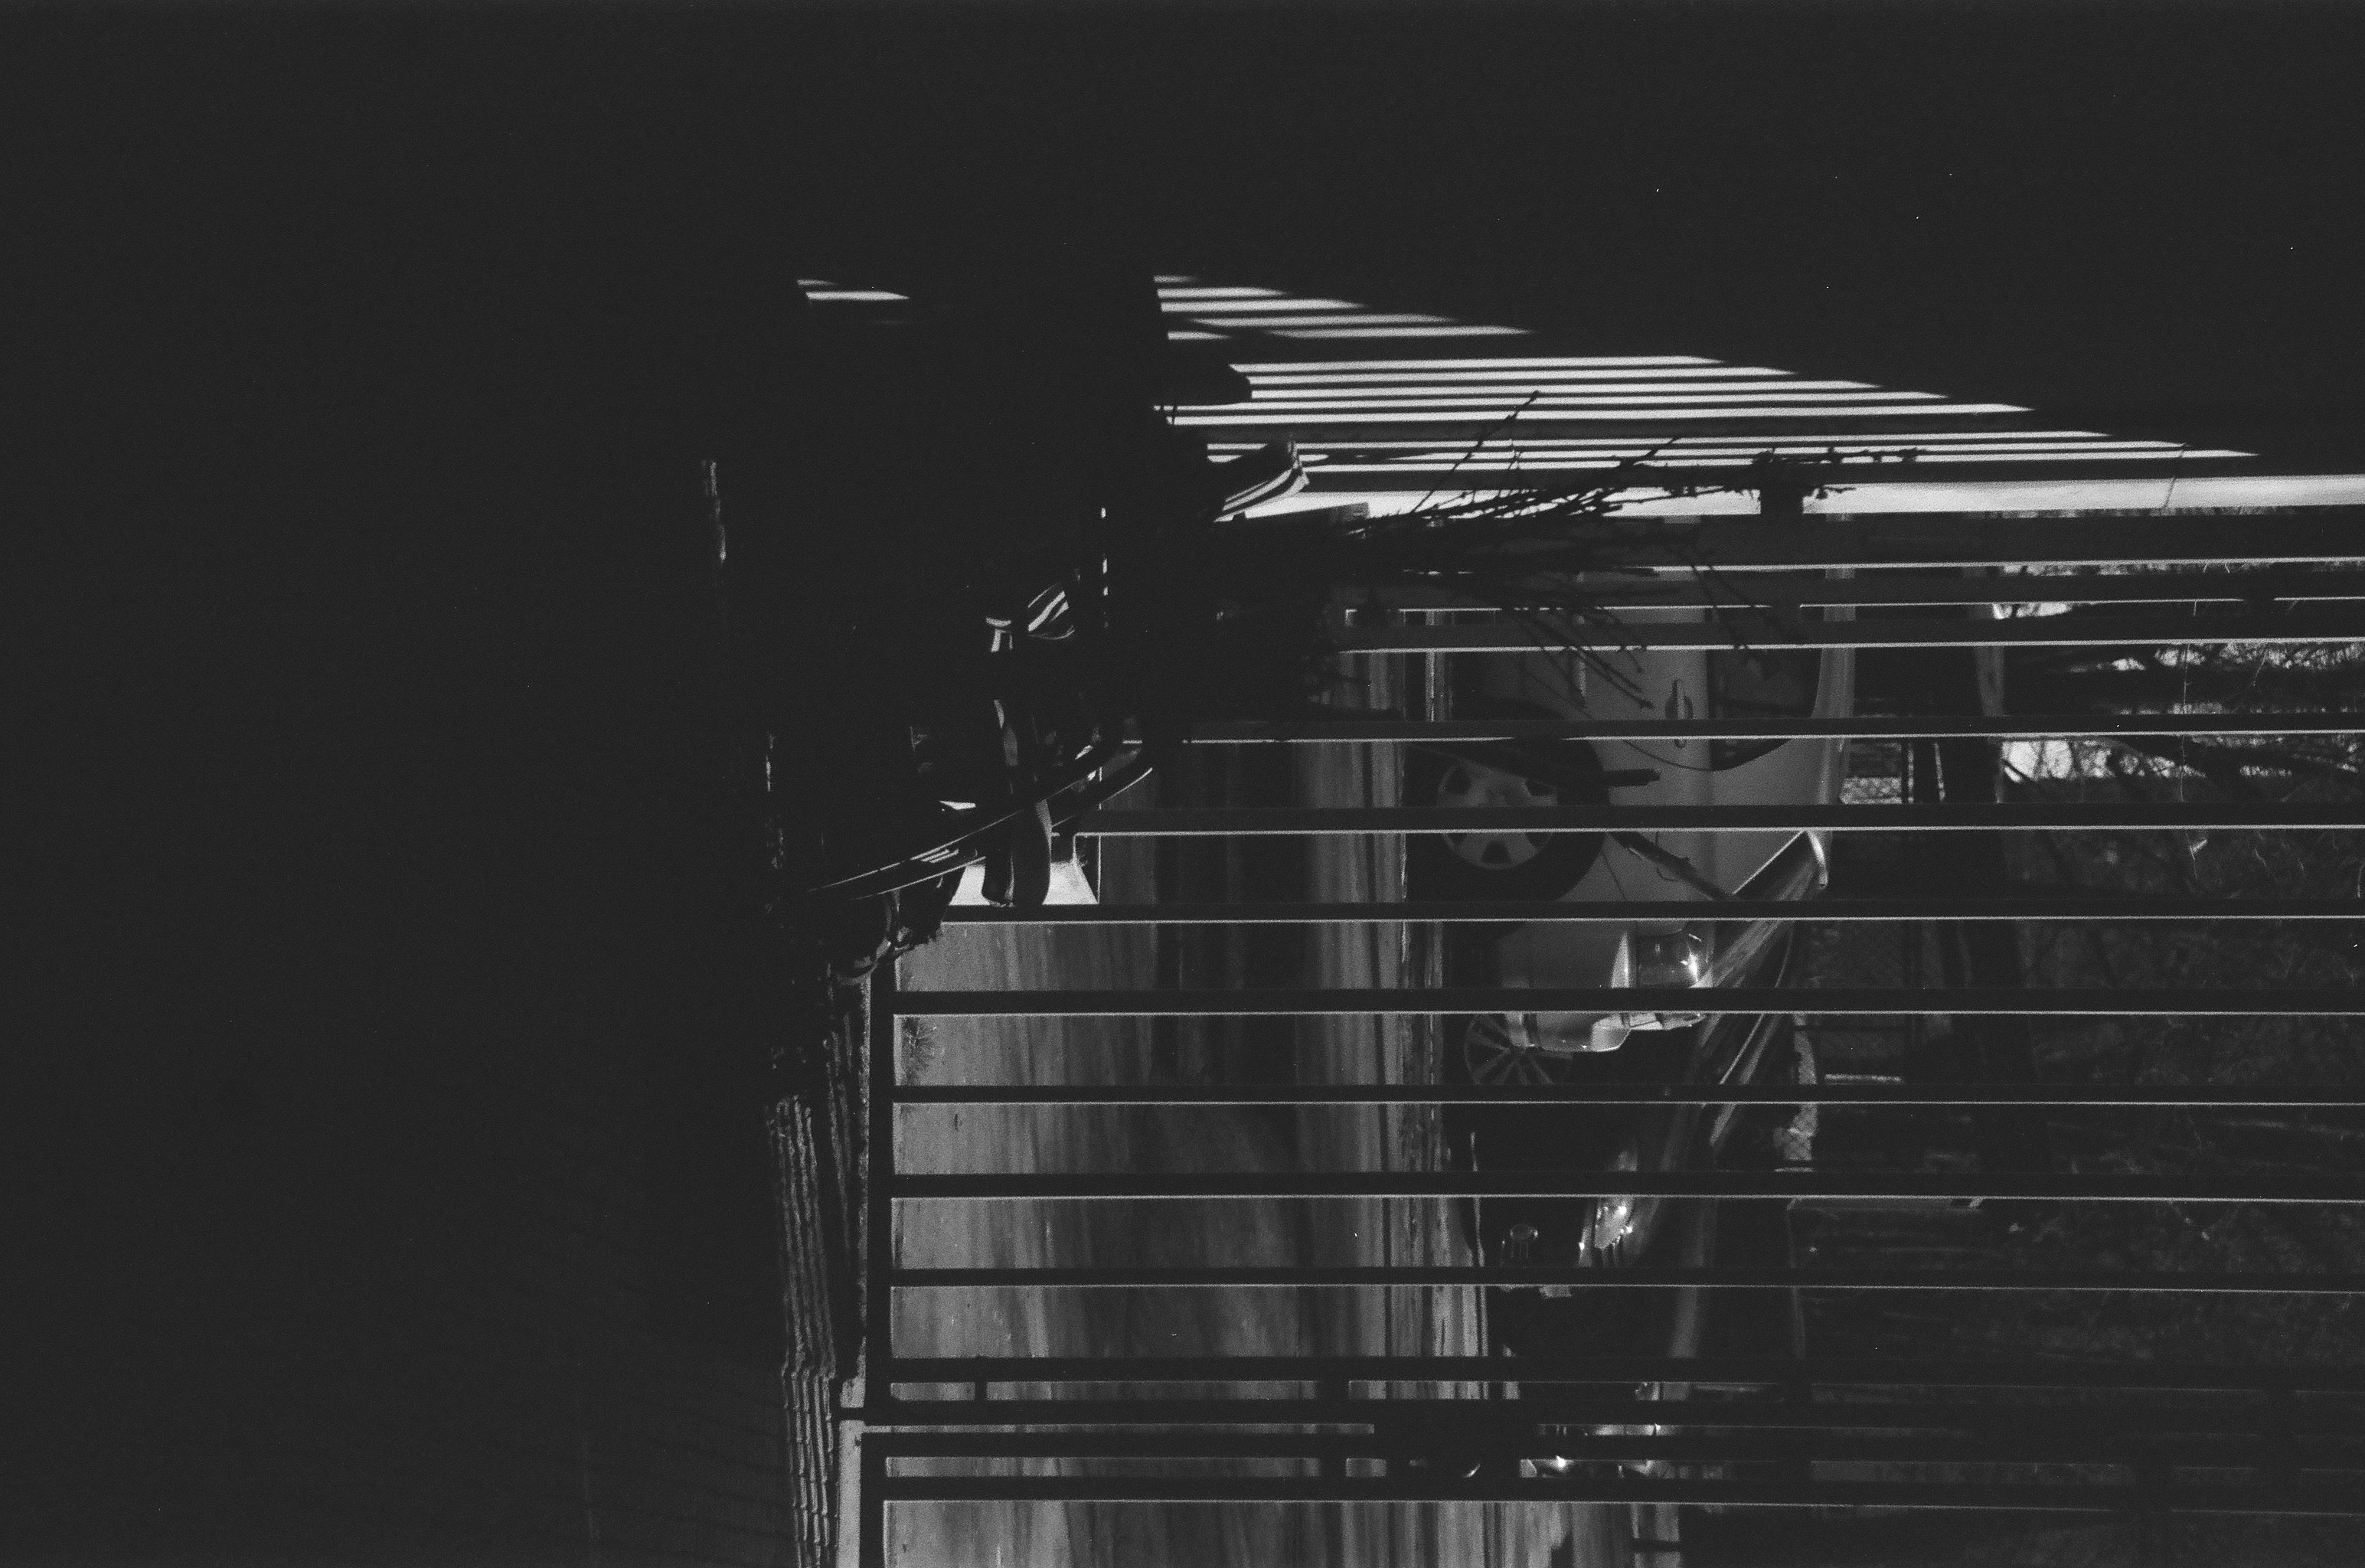
\includegraphics[angle=90, width=\linewidth, keepaspectratio]{PTI_zdjęcia_i_histogramy/photos/analog6.jpg}
    \caption{Zdjęcie niedoświetlone}
\end{figure}
\begin{figure}[H]
    \centering
    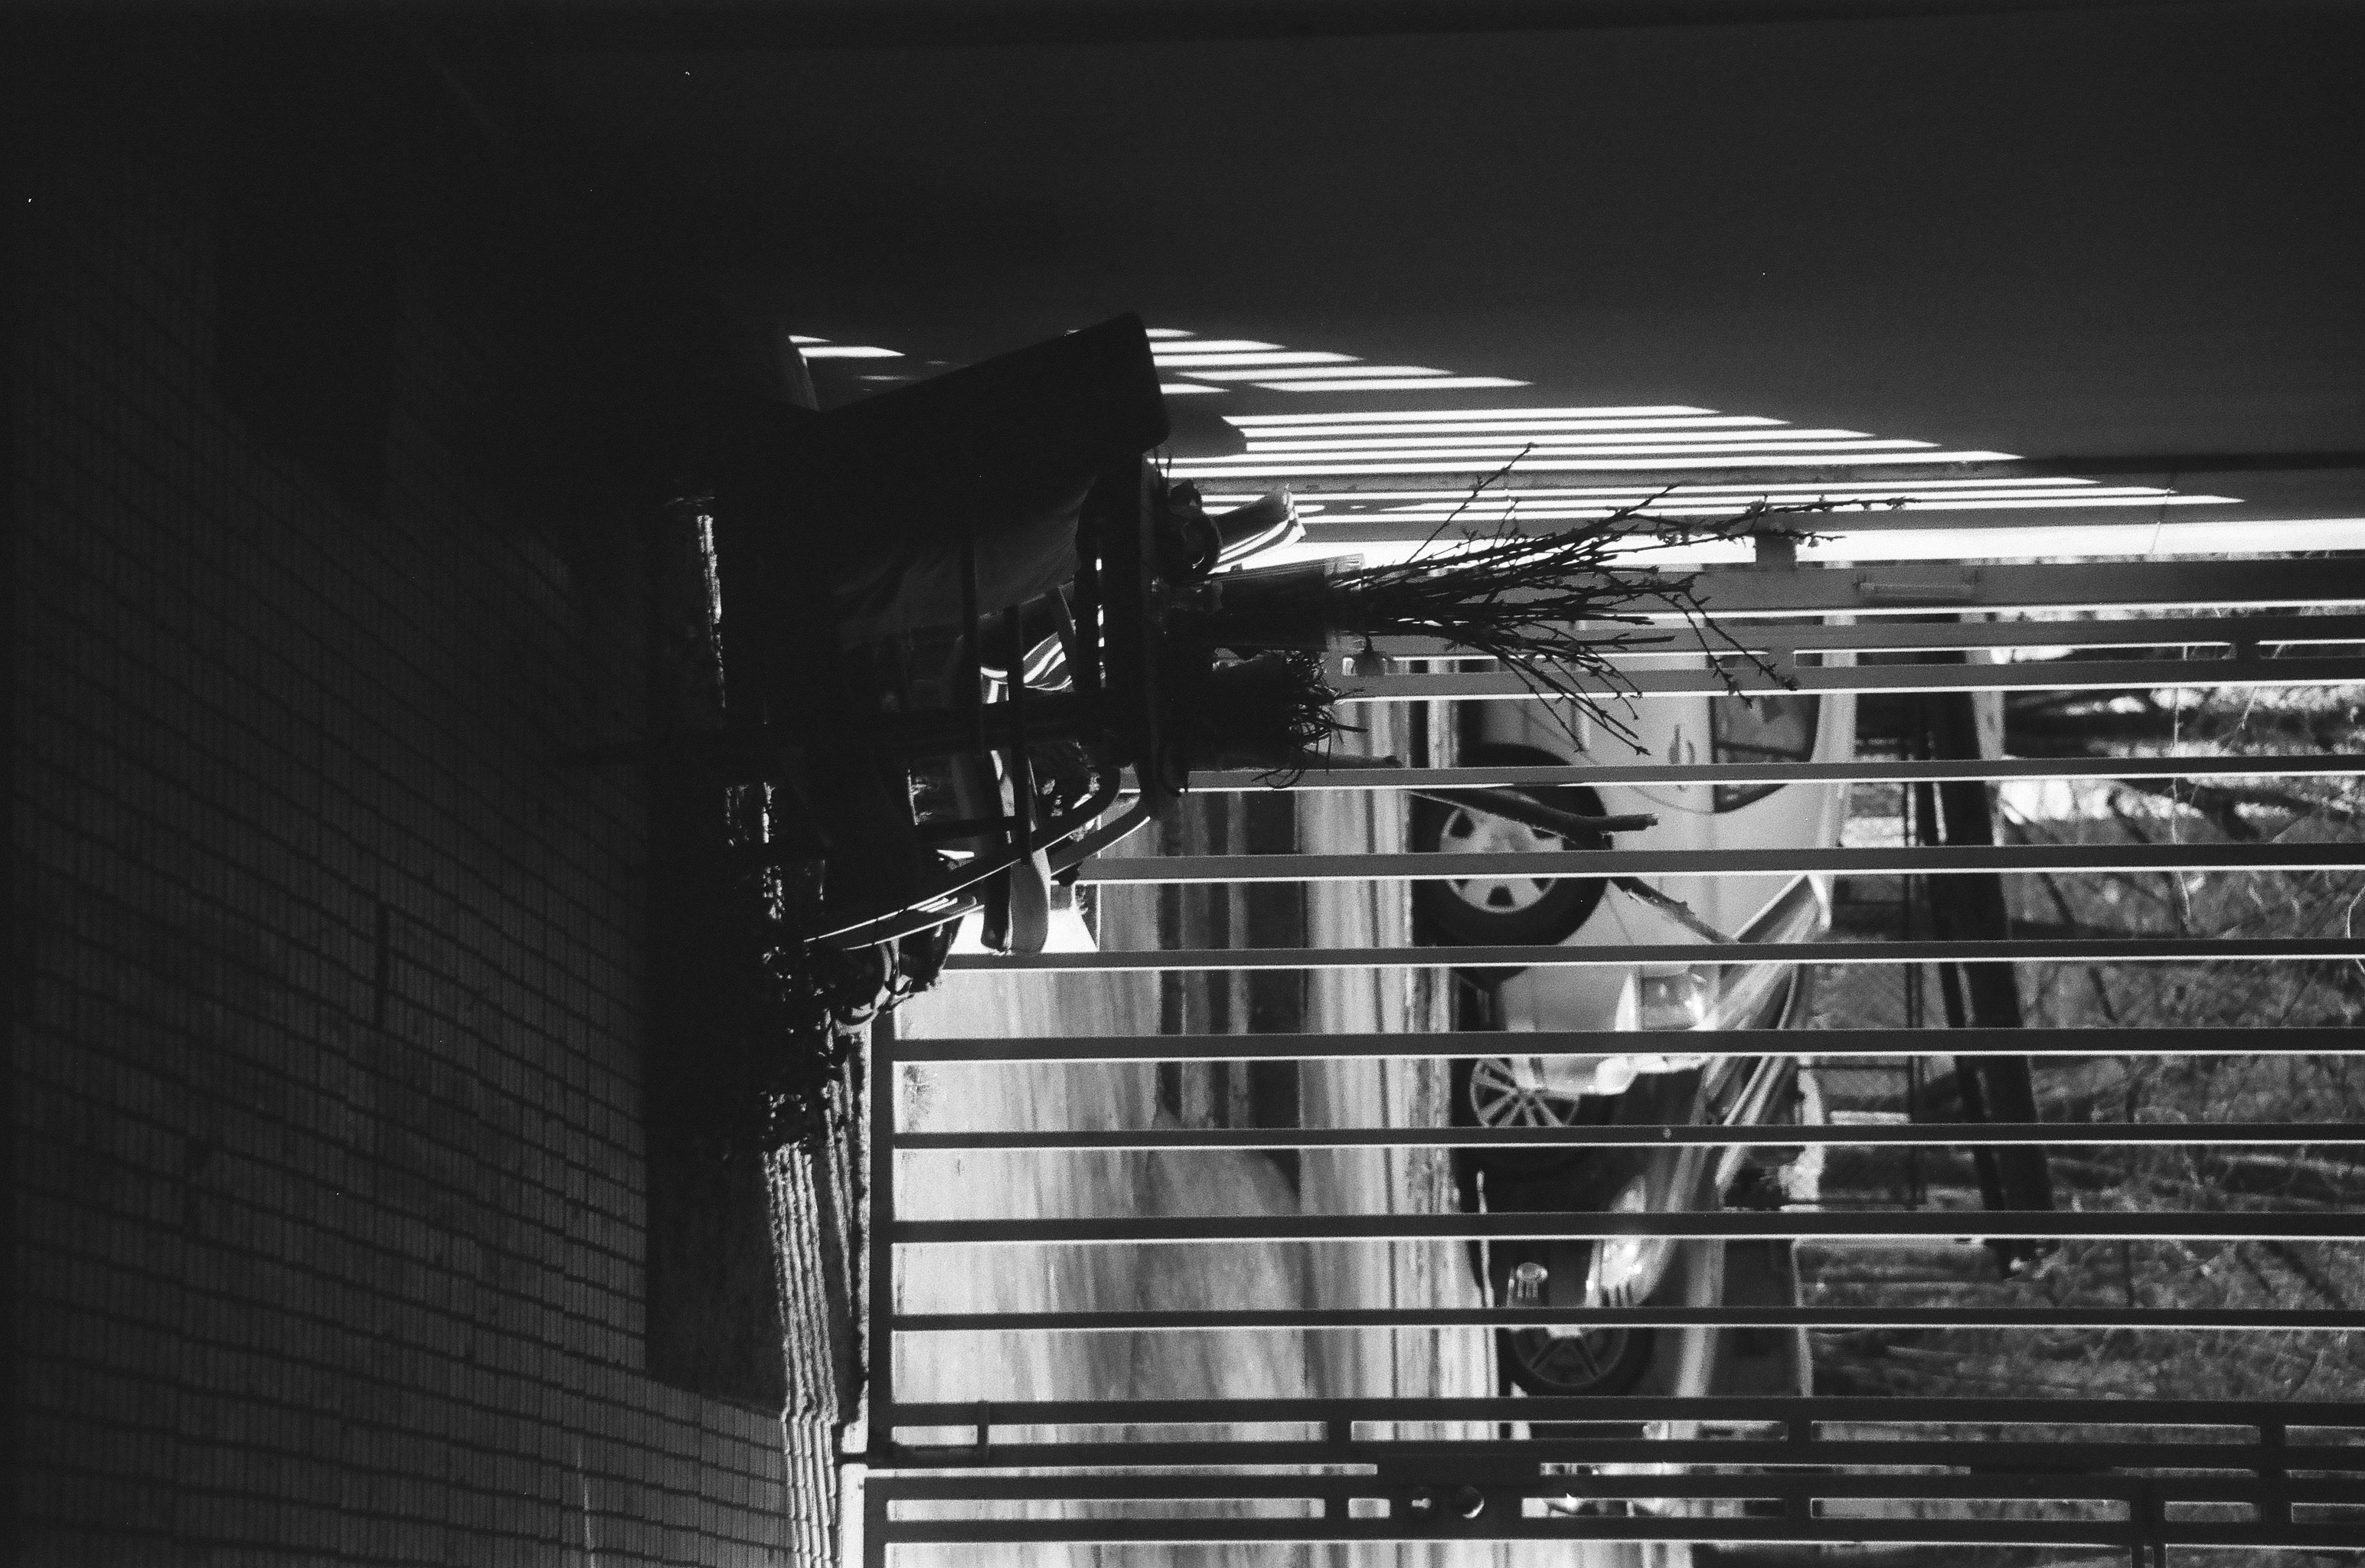
\includegraphics[angle=90, width=\linewidth, keepaspectratio]{PTI_zdjęcia_i_histogramy/photos/analog7.jpg}
    \caption{Zdjęcie doświetlone}
\end{figure}



\begin{figure}[H]
    \centering
    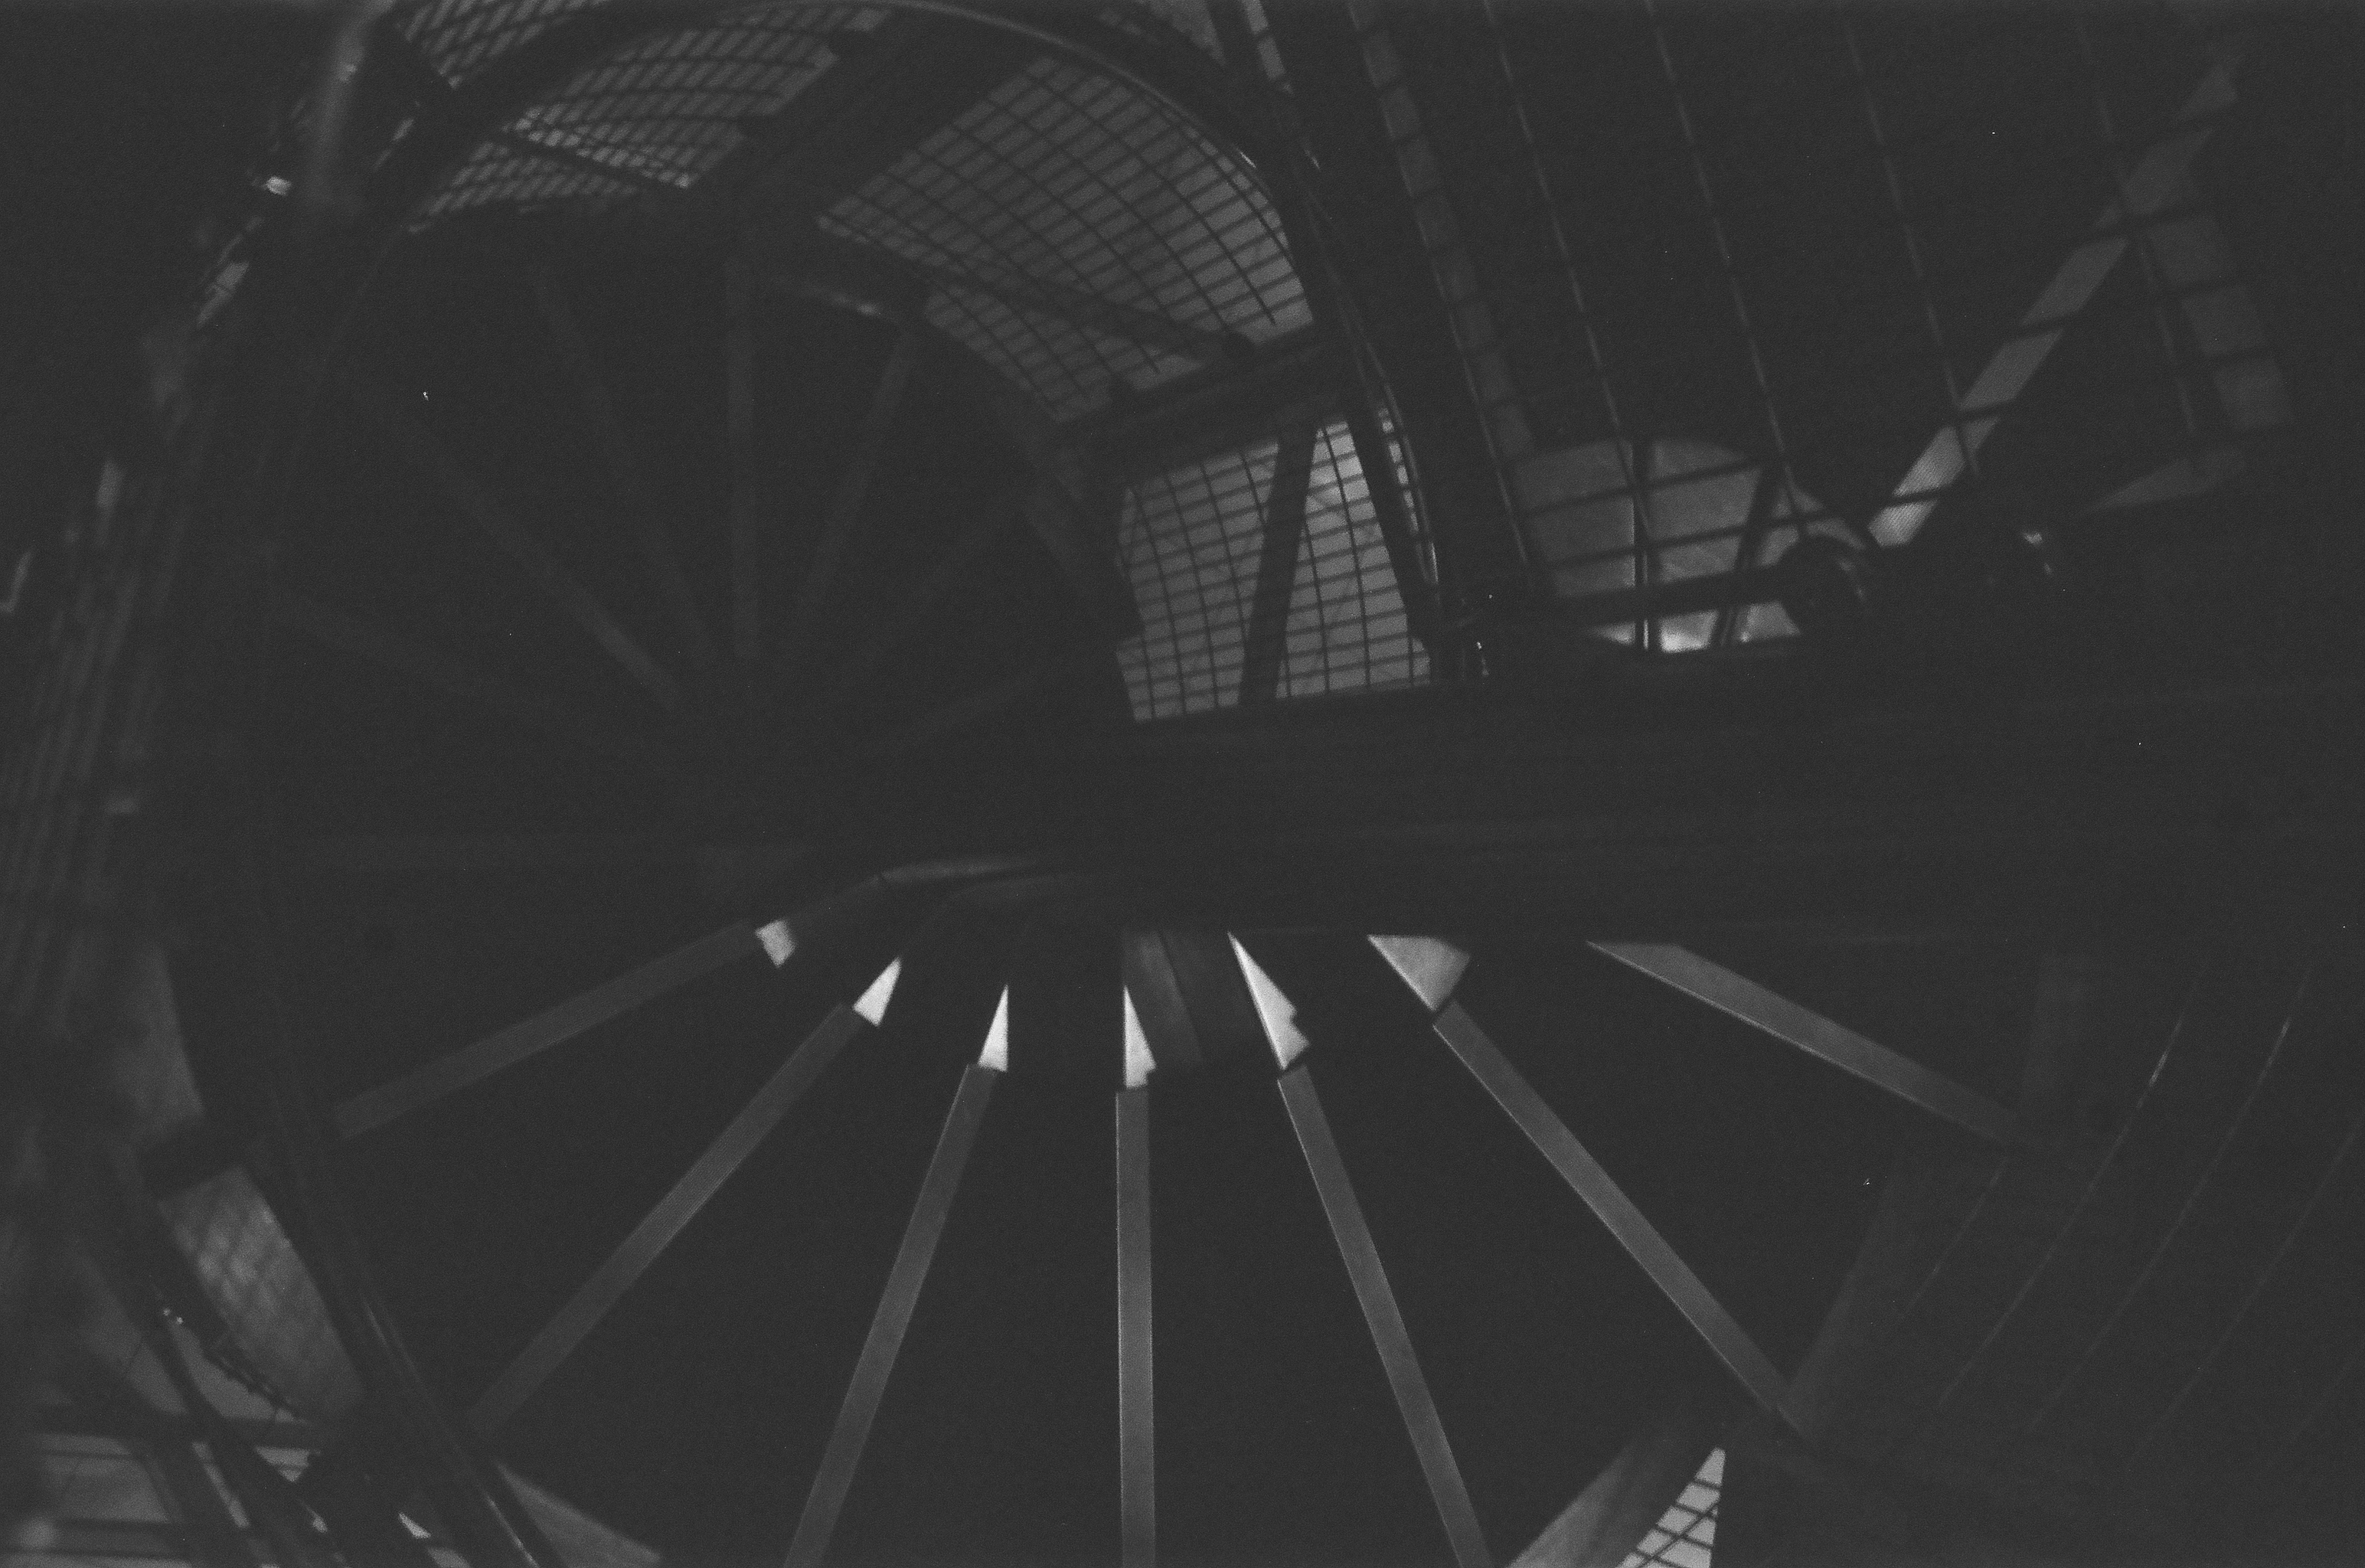
\includegraphics[angle=90, width=\linewidth, keepaspectratio]{PTI_zdjęcia_i_histogramy/photos/analog11.jpg}
    \caption{Zdjęcie niedoświetlone}
\end{figure}
\begin{figure}[H]
    \centering
    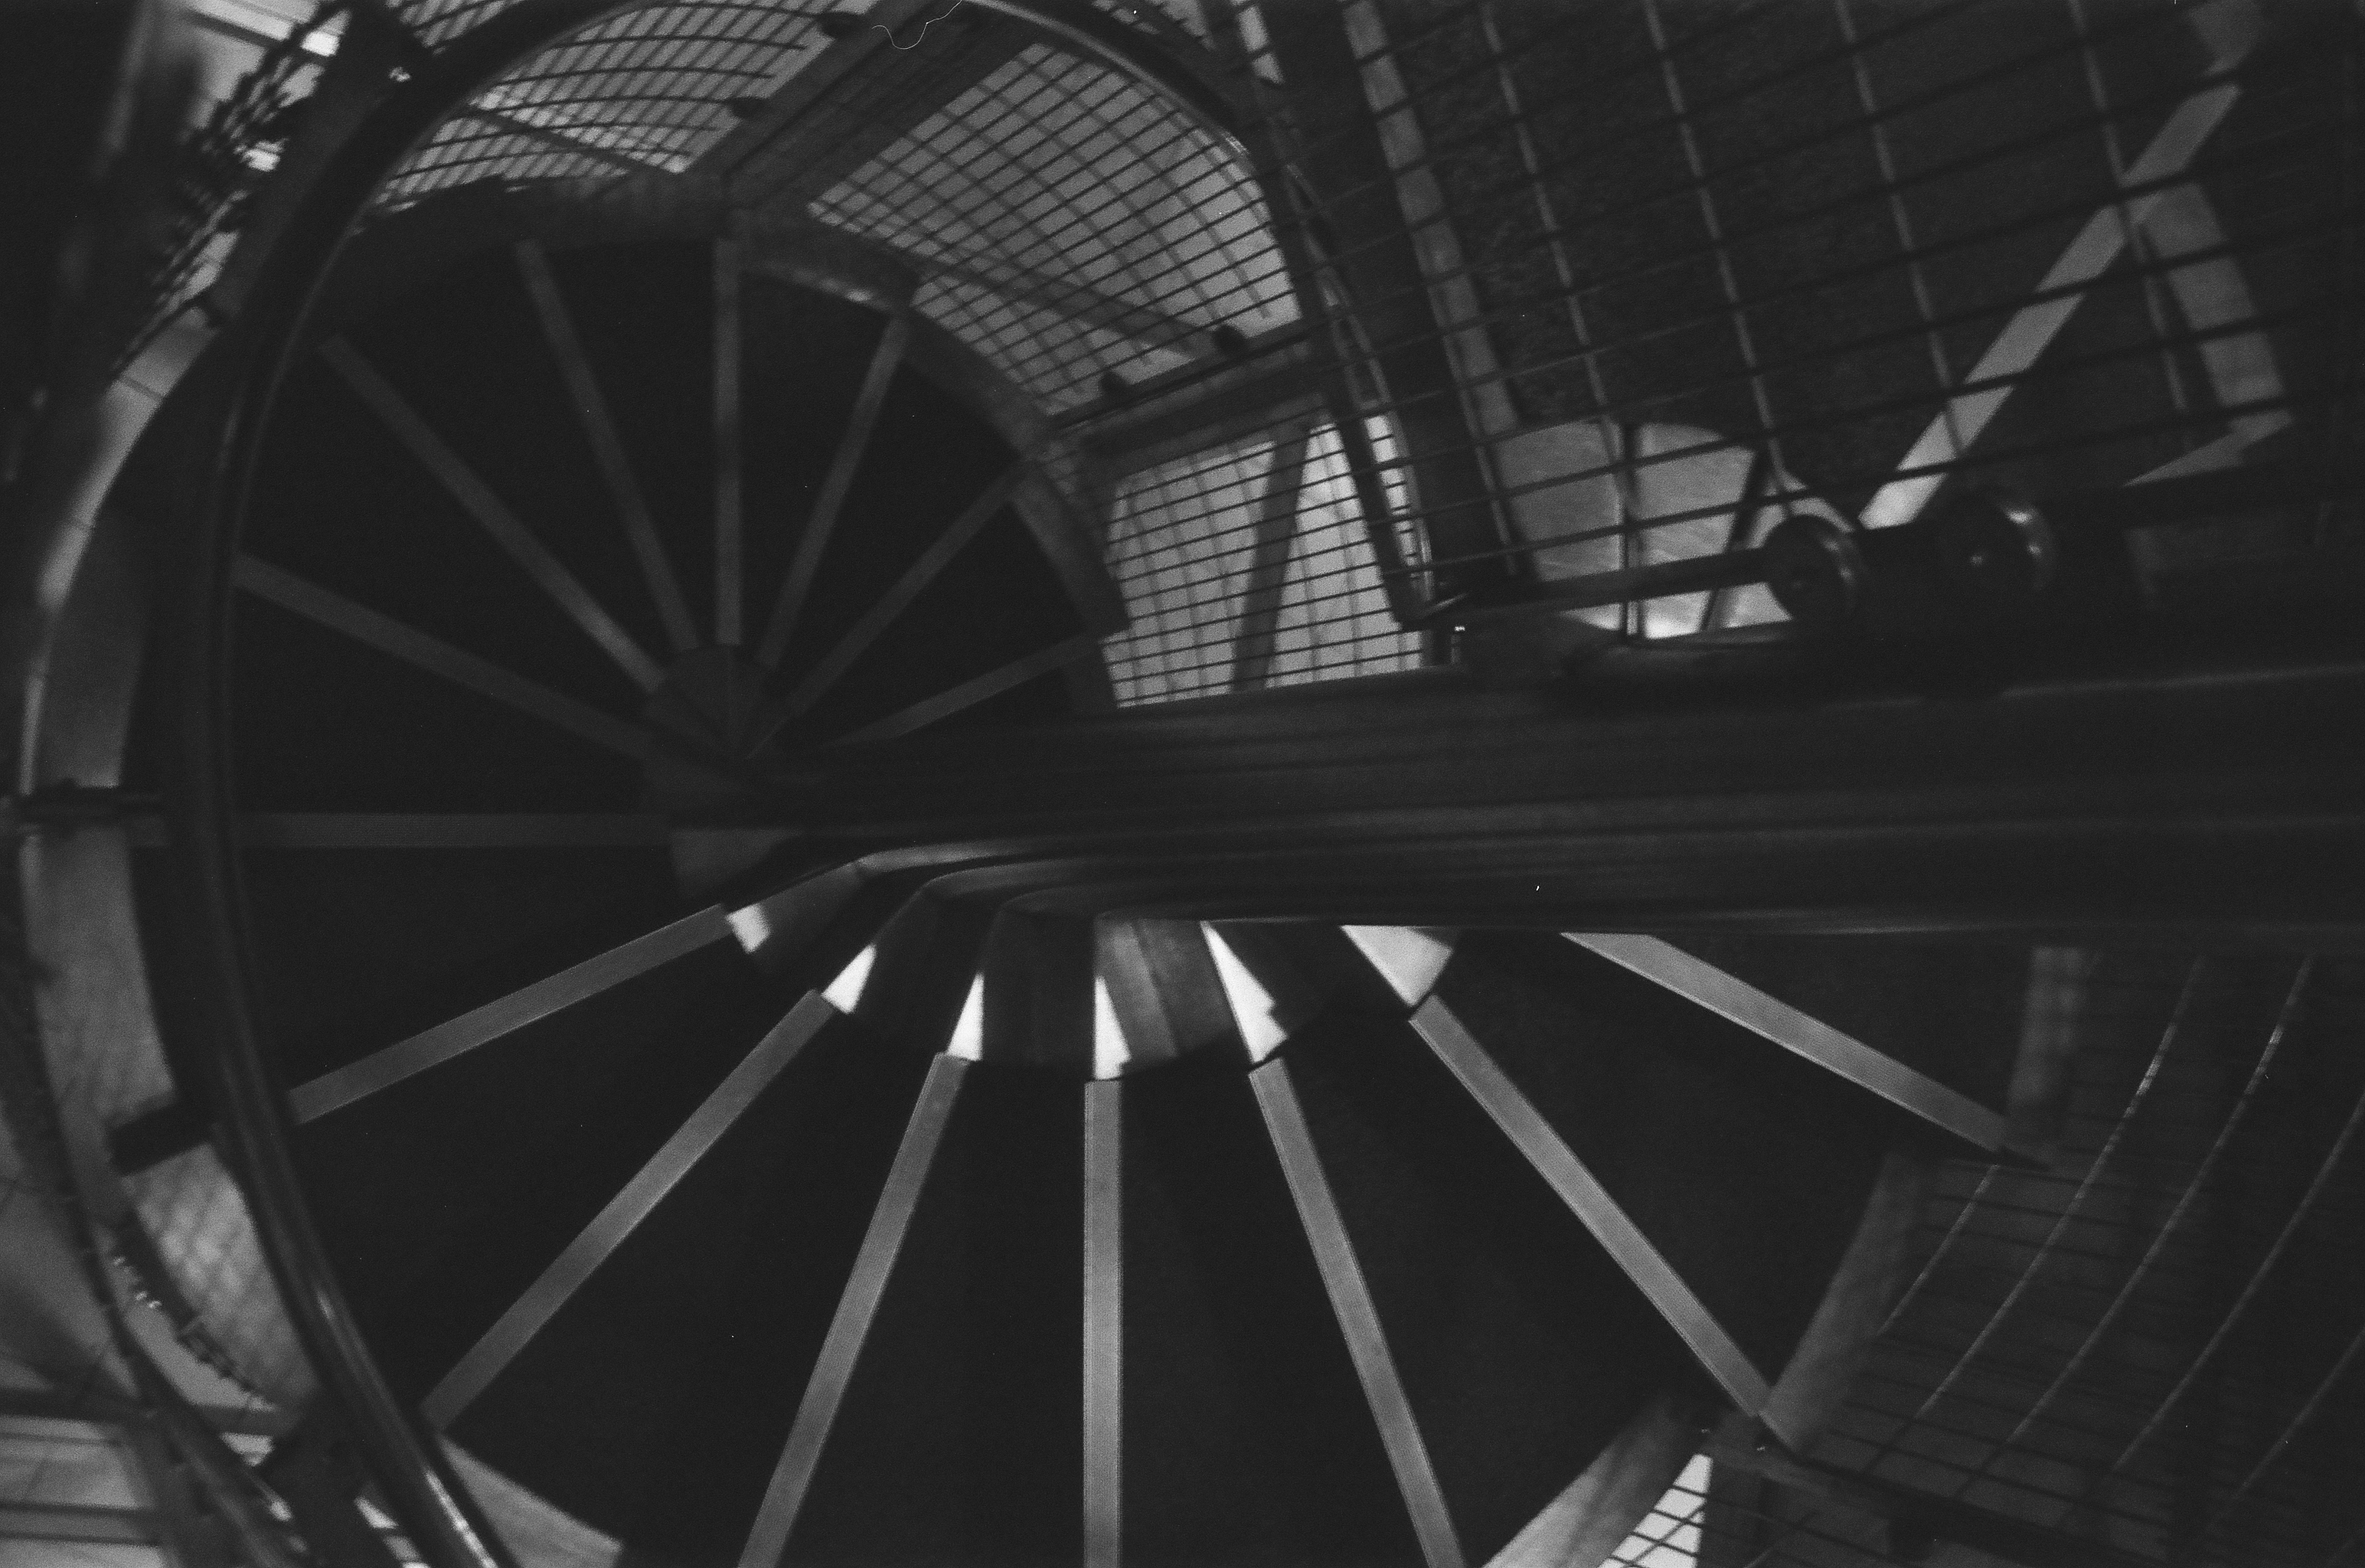
\includegraphics[angle=90, width=\linewidth, keepaspectratio]{PTI_zdjęcia_i_histogramy/photos/analog14.jpg}
    \caption{Zdjęcie doświetlone}
\end{figure}



\begin{figure}[H]
    \centering
    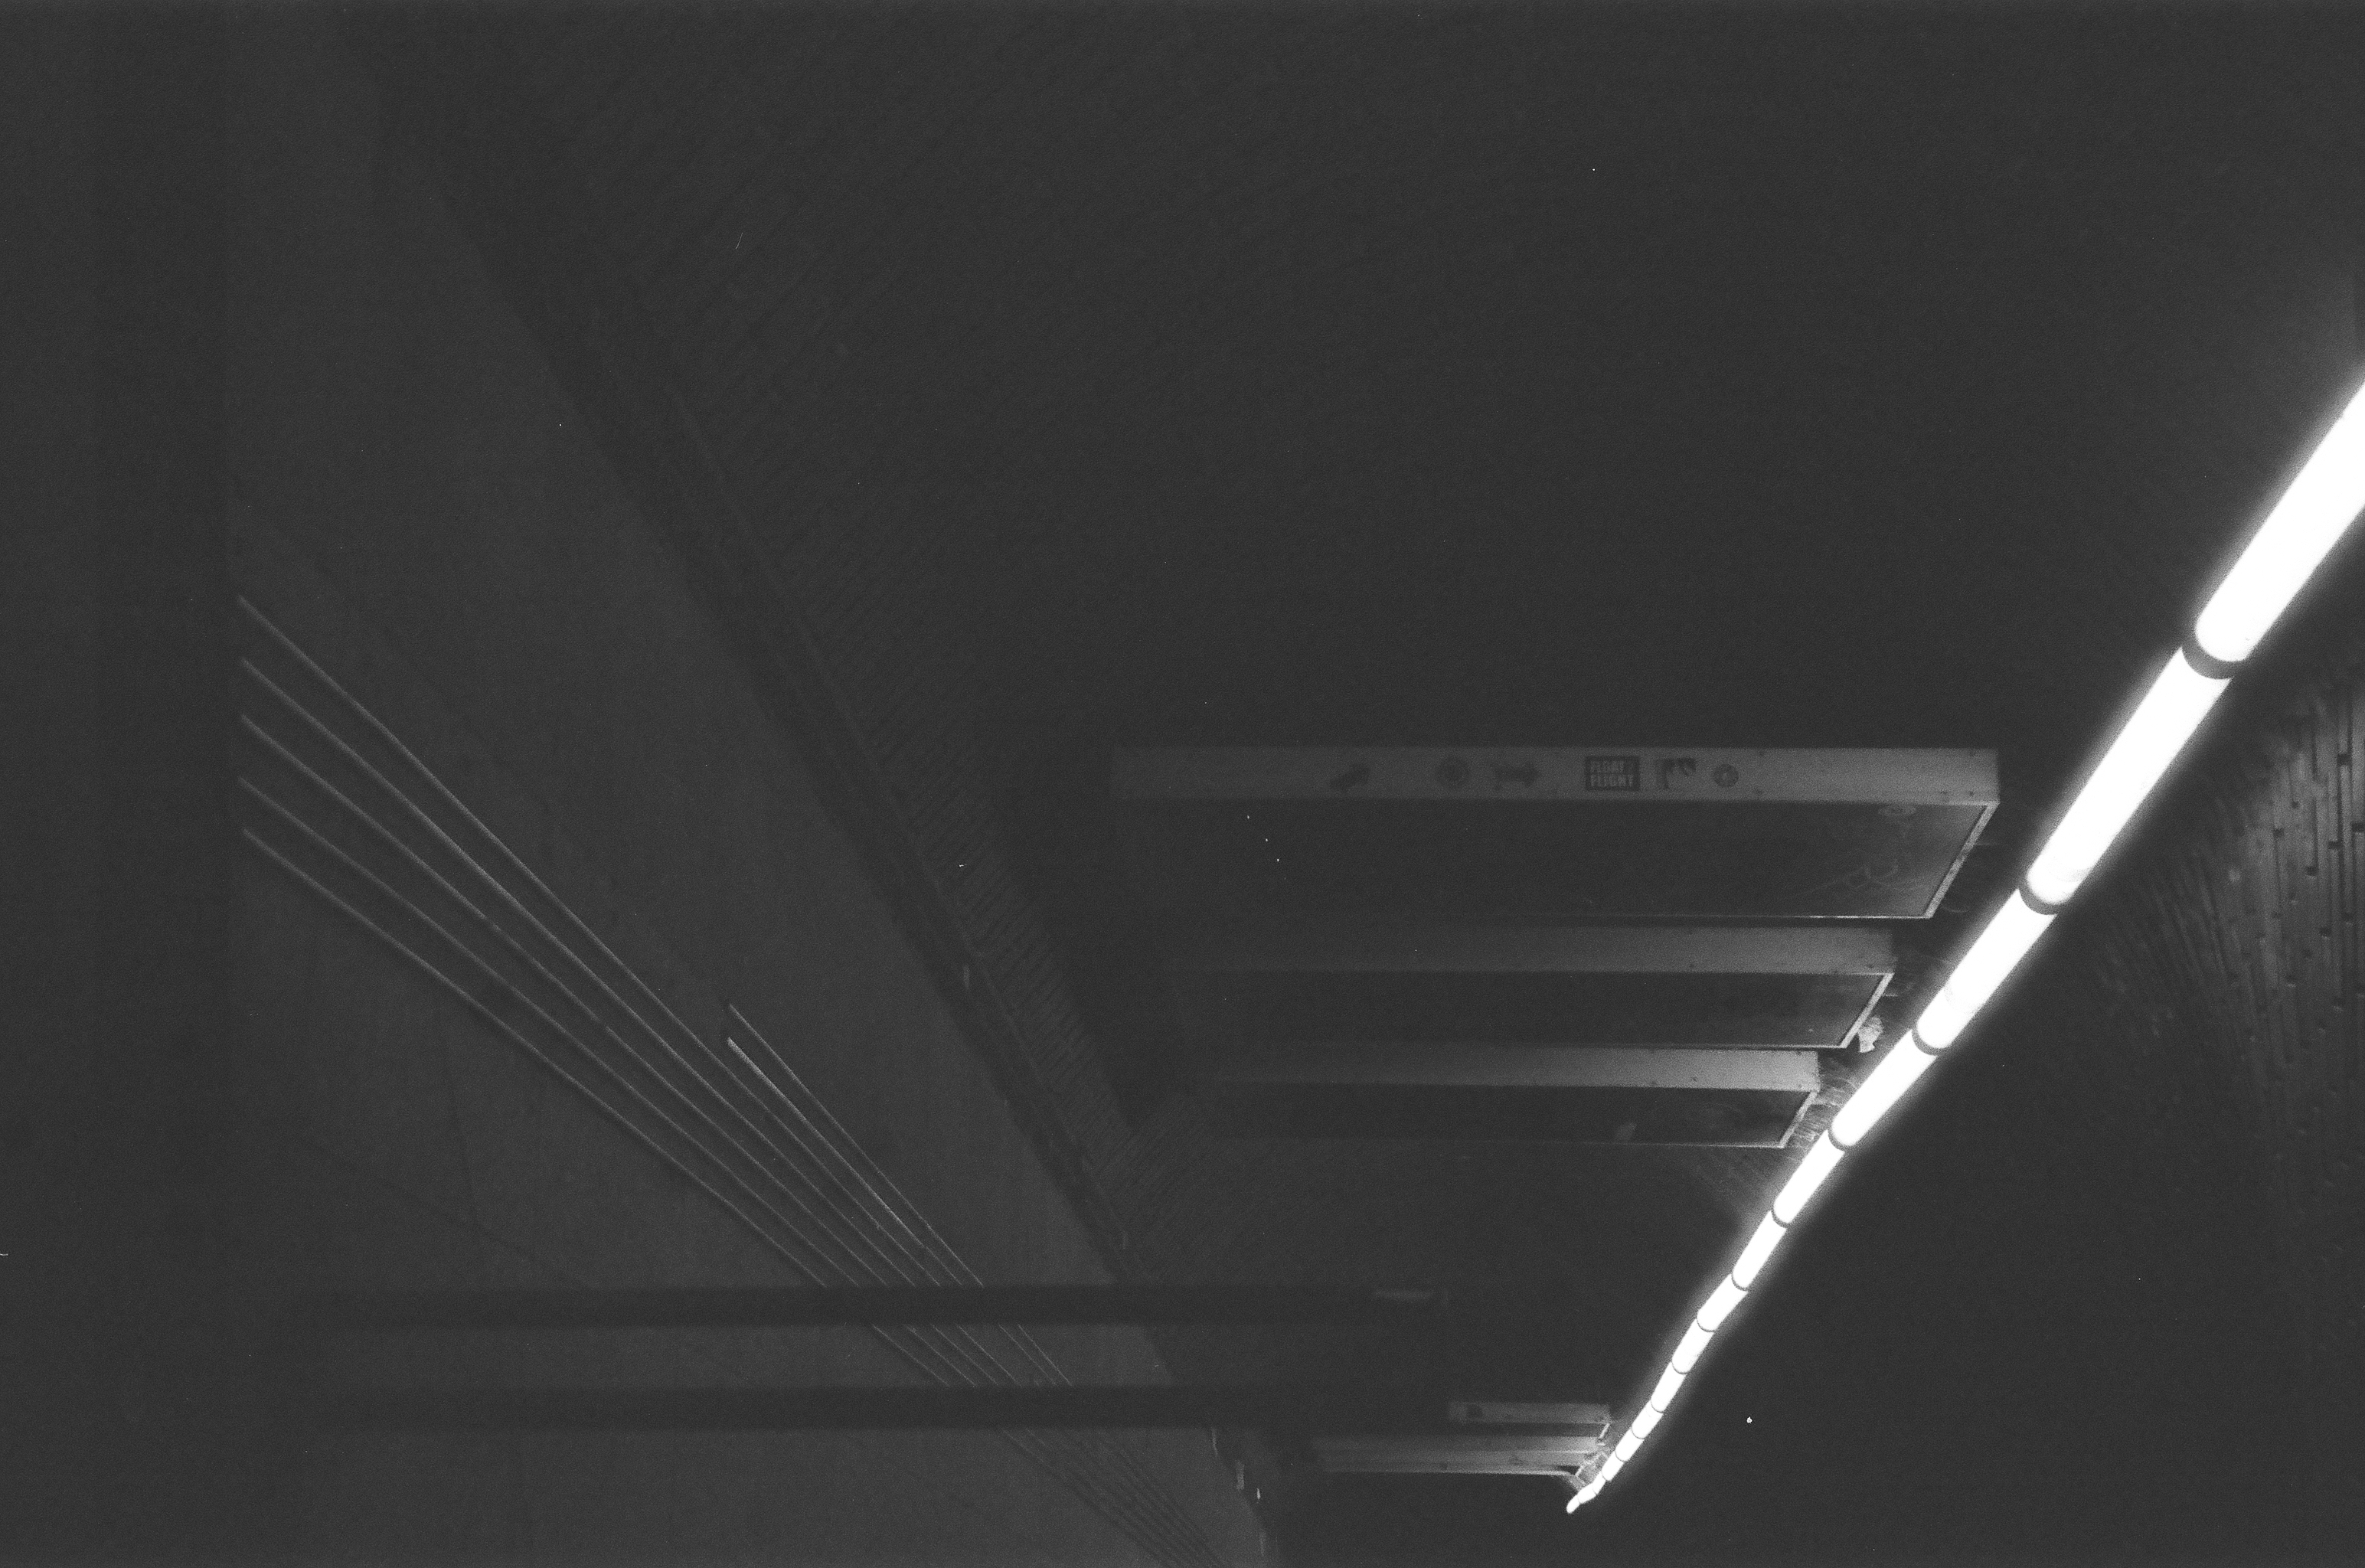
\includegraphics[angle=90, width=\linewidth, keepaspectratio]{PTI_zdjęcia_i_histogramy/photos/analog23.jpg}
    \caption{Zdjęcie niedoświetlone}
\end{figure}
\begin{figure}[H]
    \centering
    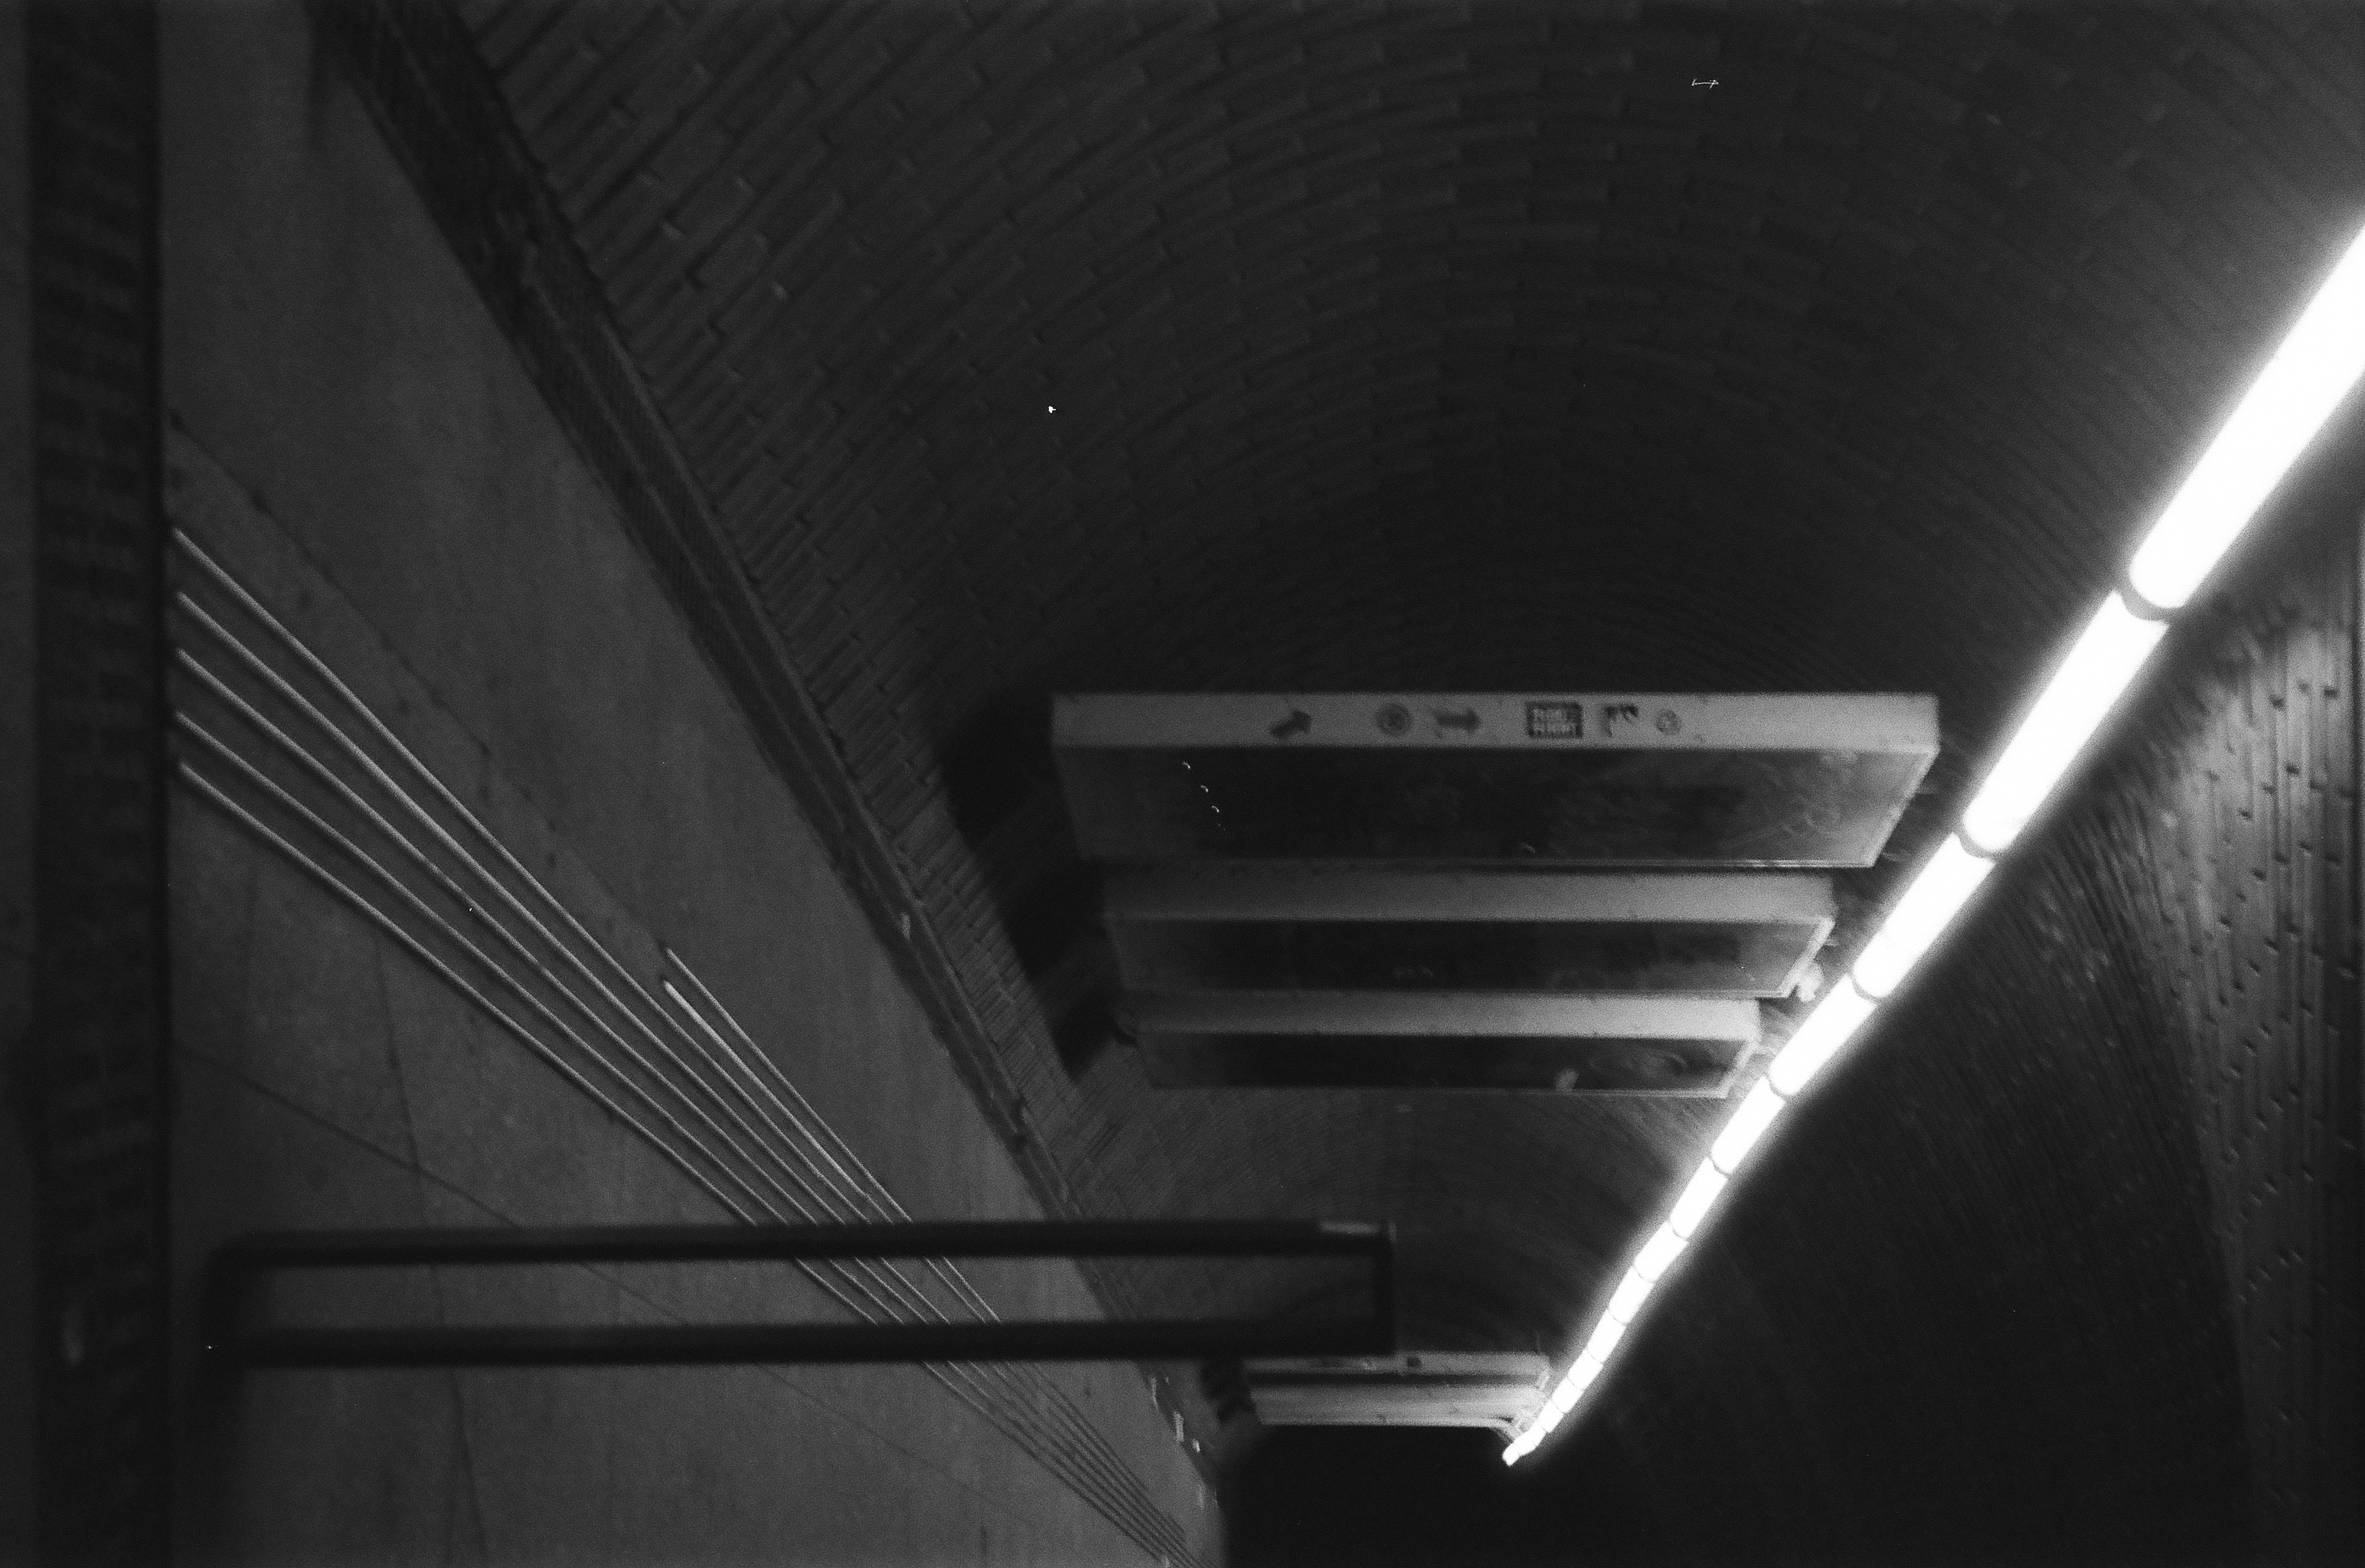
\includegraphics[angle=90, width=\linewidth, keepaspectratio]{PTI_zdjęcia_i_histogramy/photos/analog22.jpg}
    \caption{Zdjęcie doświetlone}
\end{figure}


\begin{figure}[H]
    \centering
    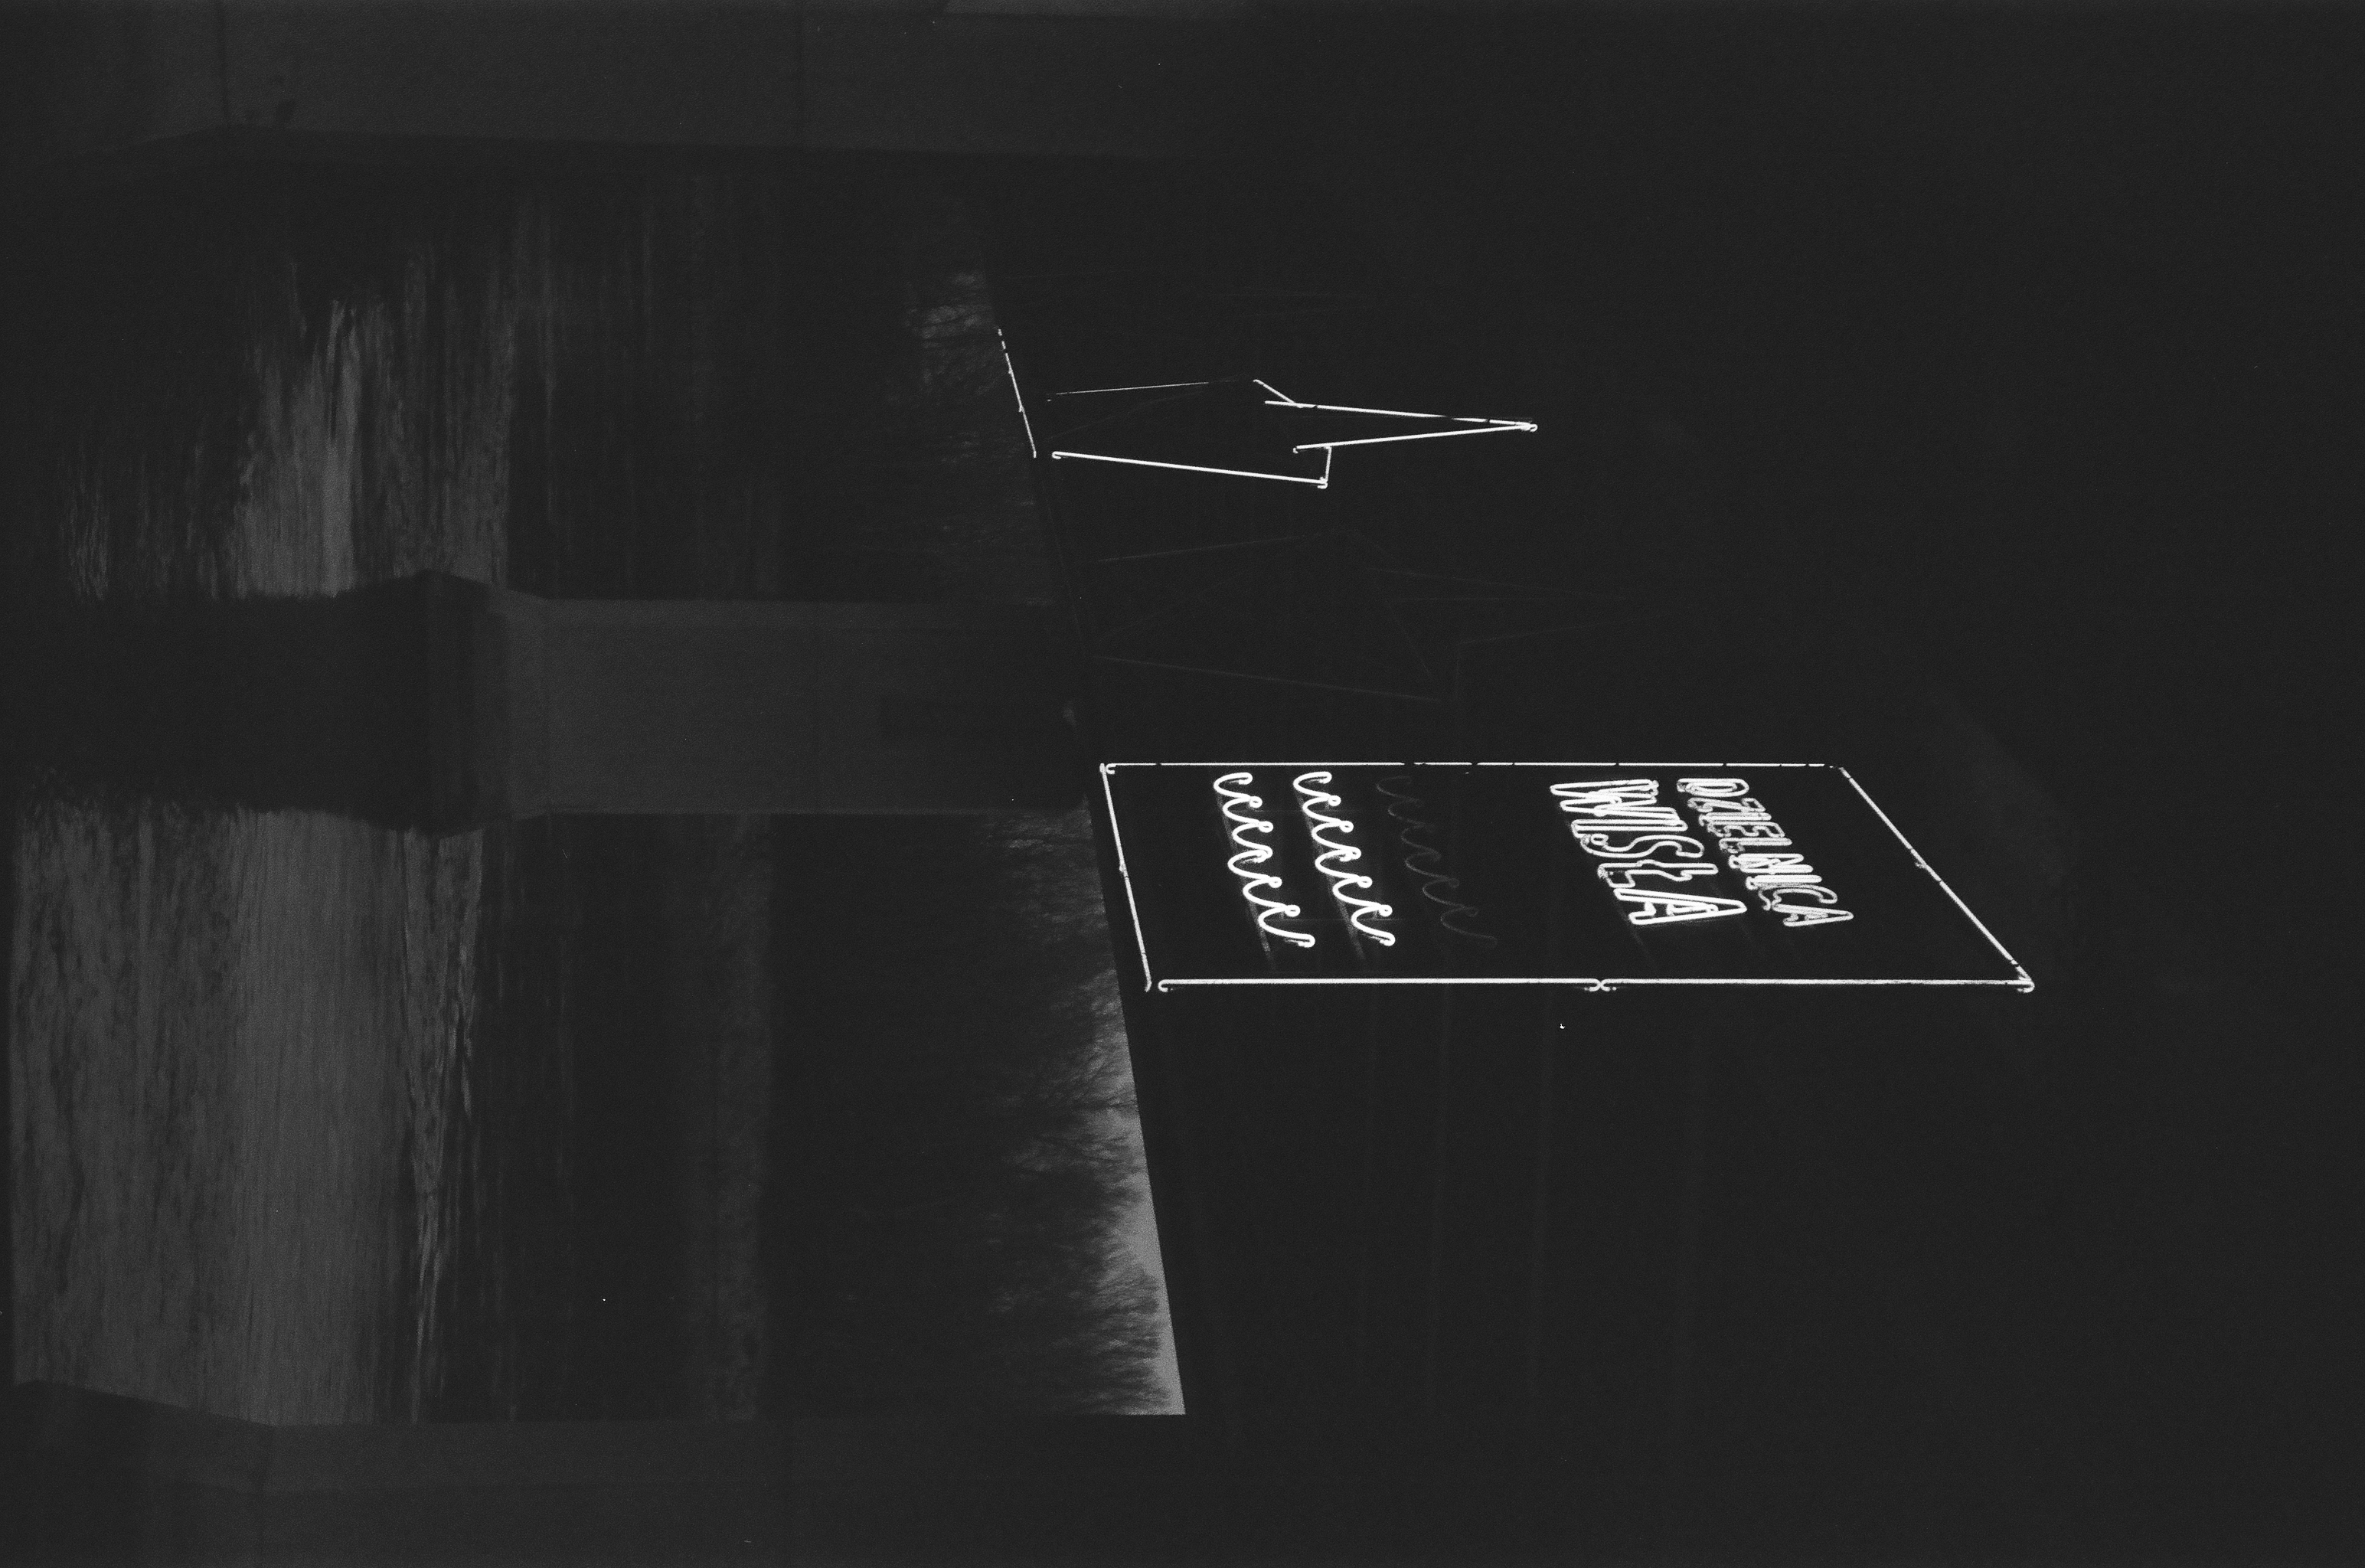
\includegraphics[angle=90, width=\linewidth, keepaspectratio]{PTI_zdjęcia_i_histogramy/photos/analog35.jpg}
    \caption{Zdjęcie niedoświetlone}
\end{figure}
\begin{figure}[H]
    \centering
    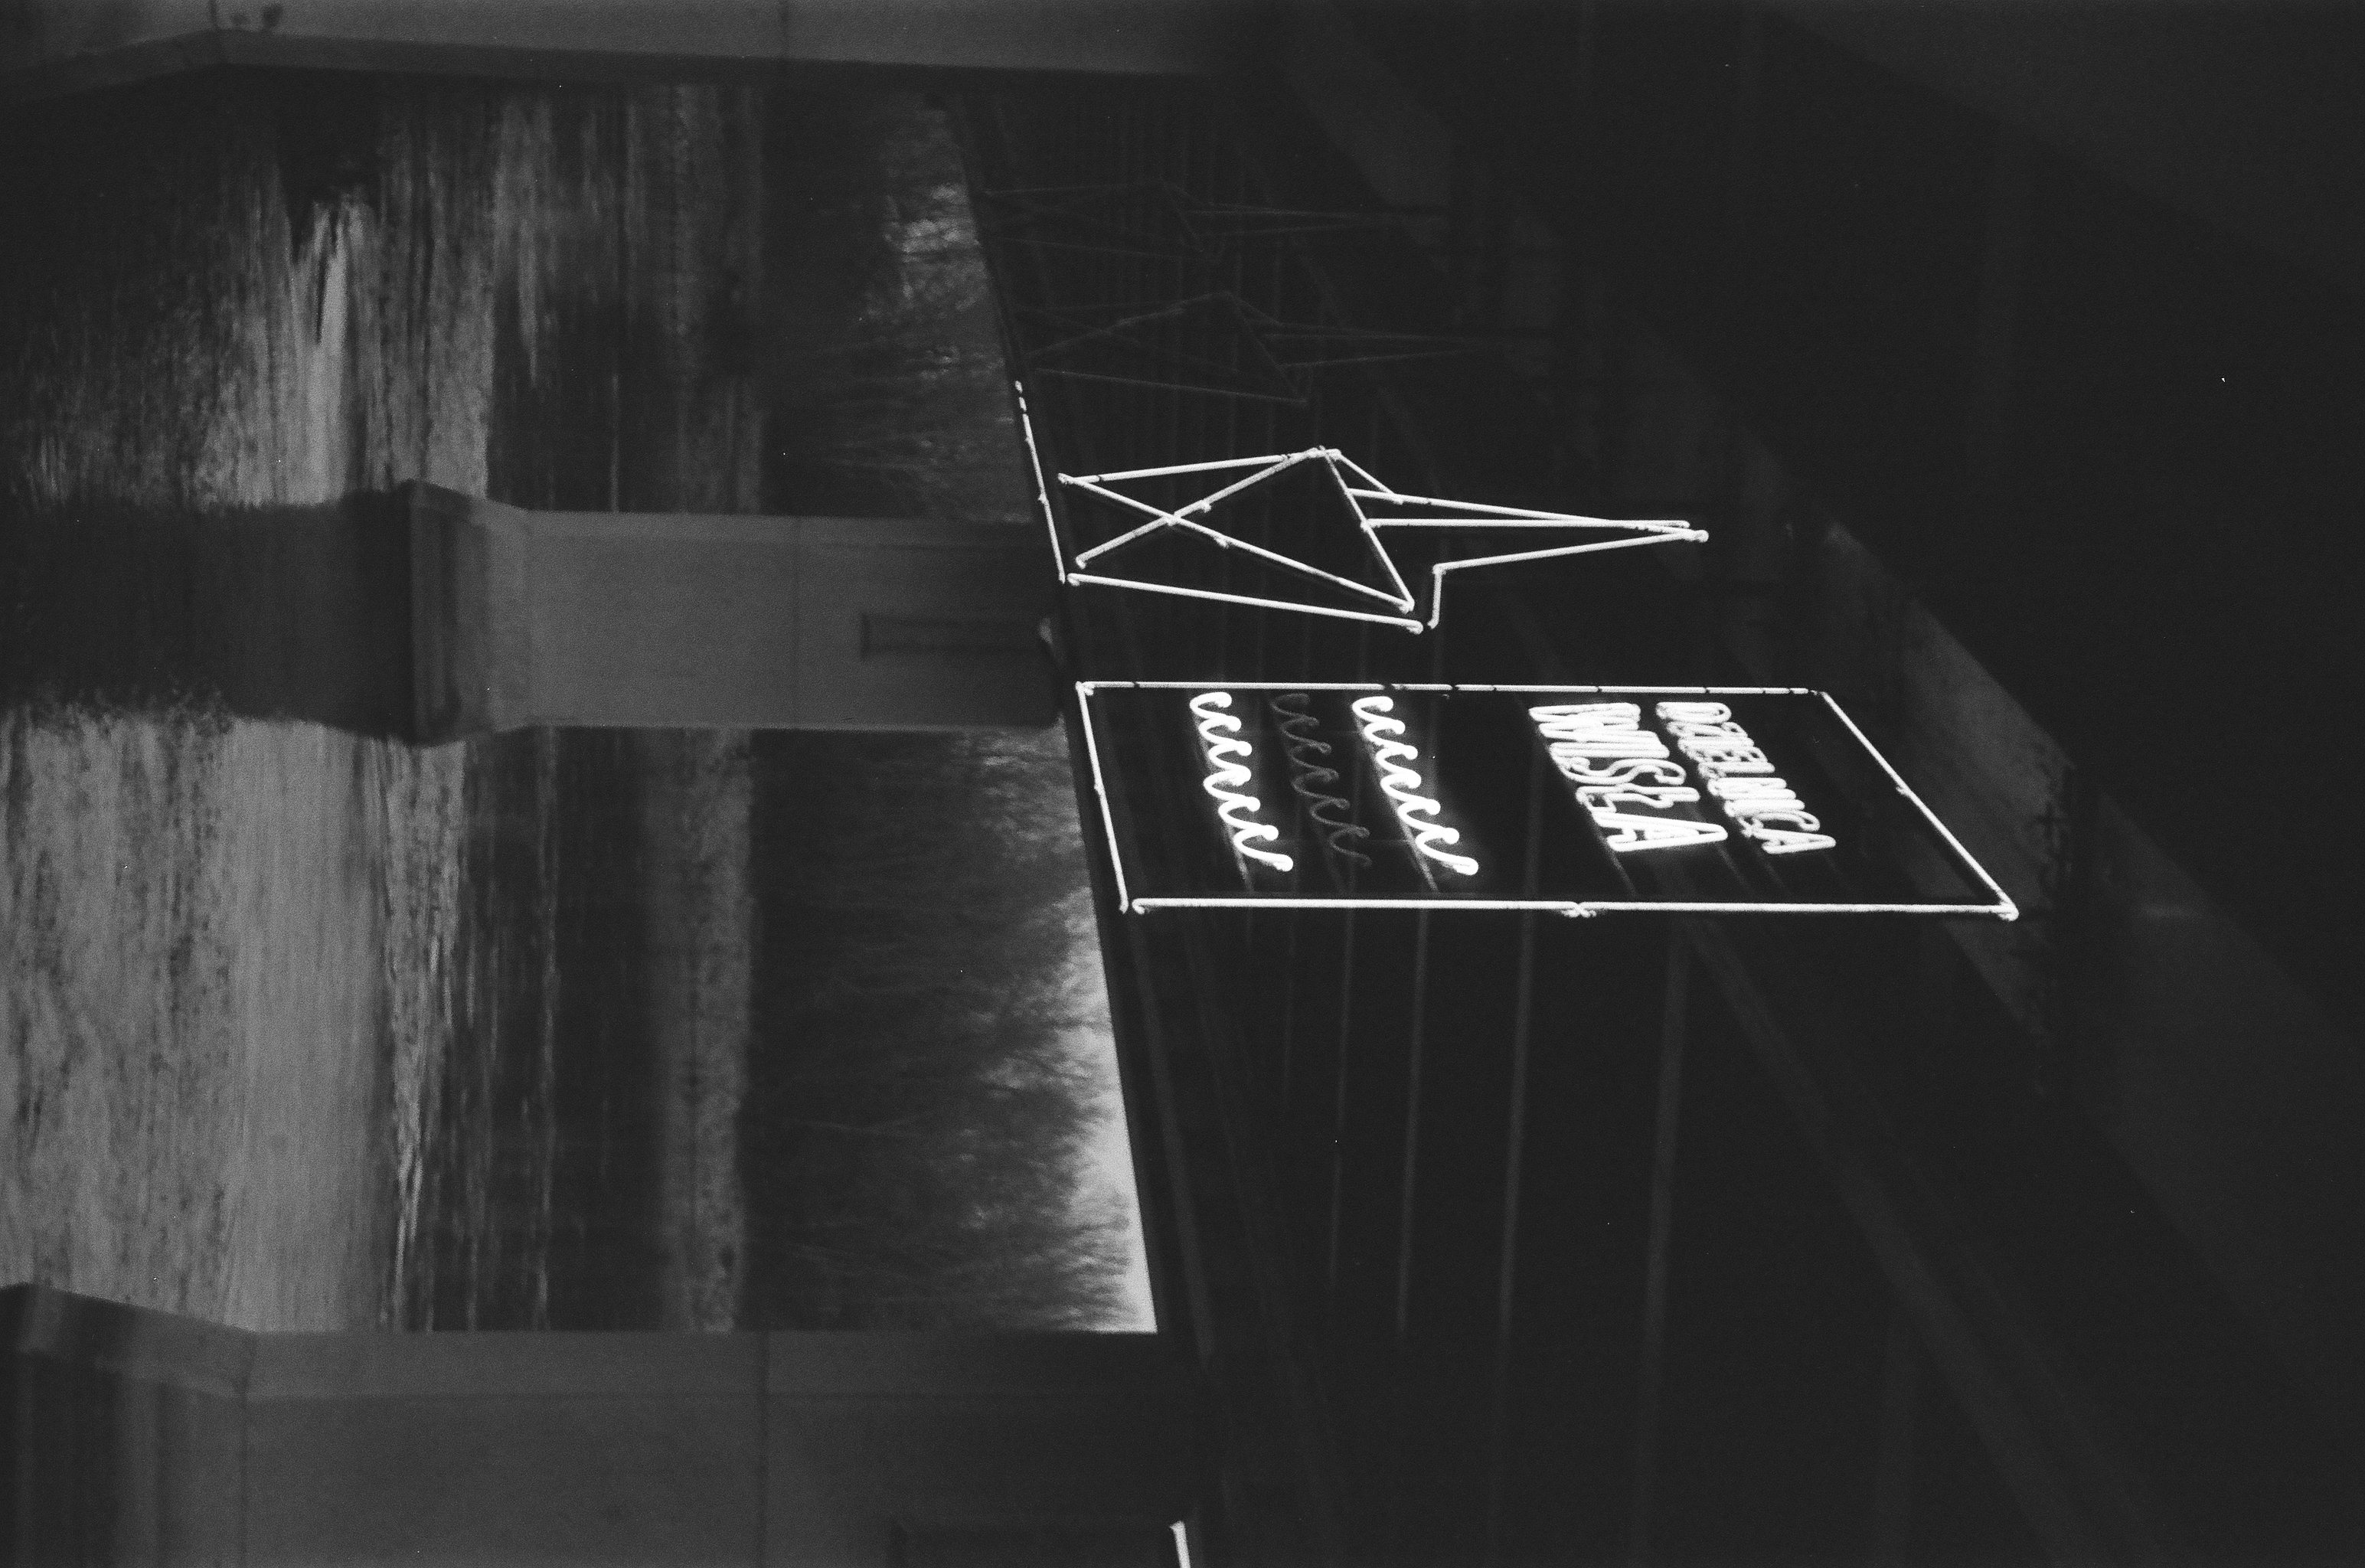
\includegraphics[angle=90, width=\linewidth, keepaspectratio]{PTI_zdjęcia_i_histogramy/photos/analog36.jpg}
    \caption{Zdjęcie doświetlone}
\end{figure}


\newpage
A także w przypadku fotografii cyfrowej:

\begin{figure}[H]
    \centering
    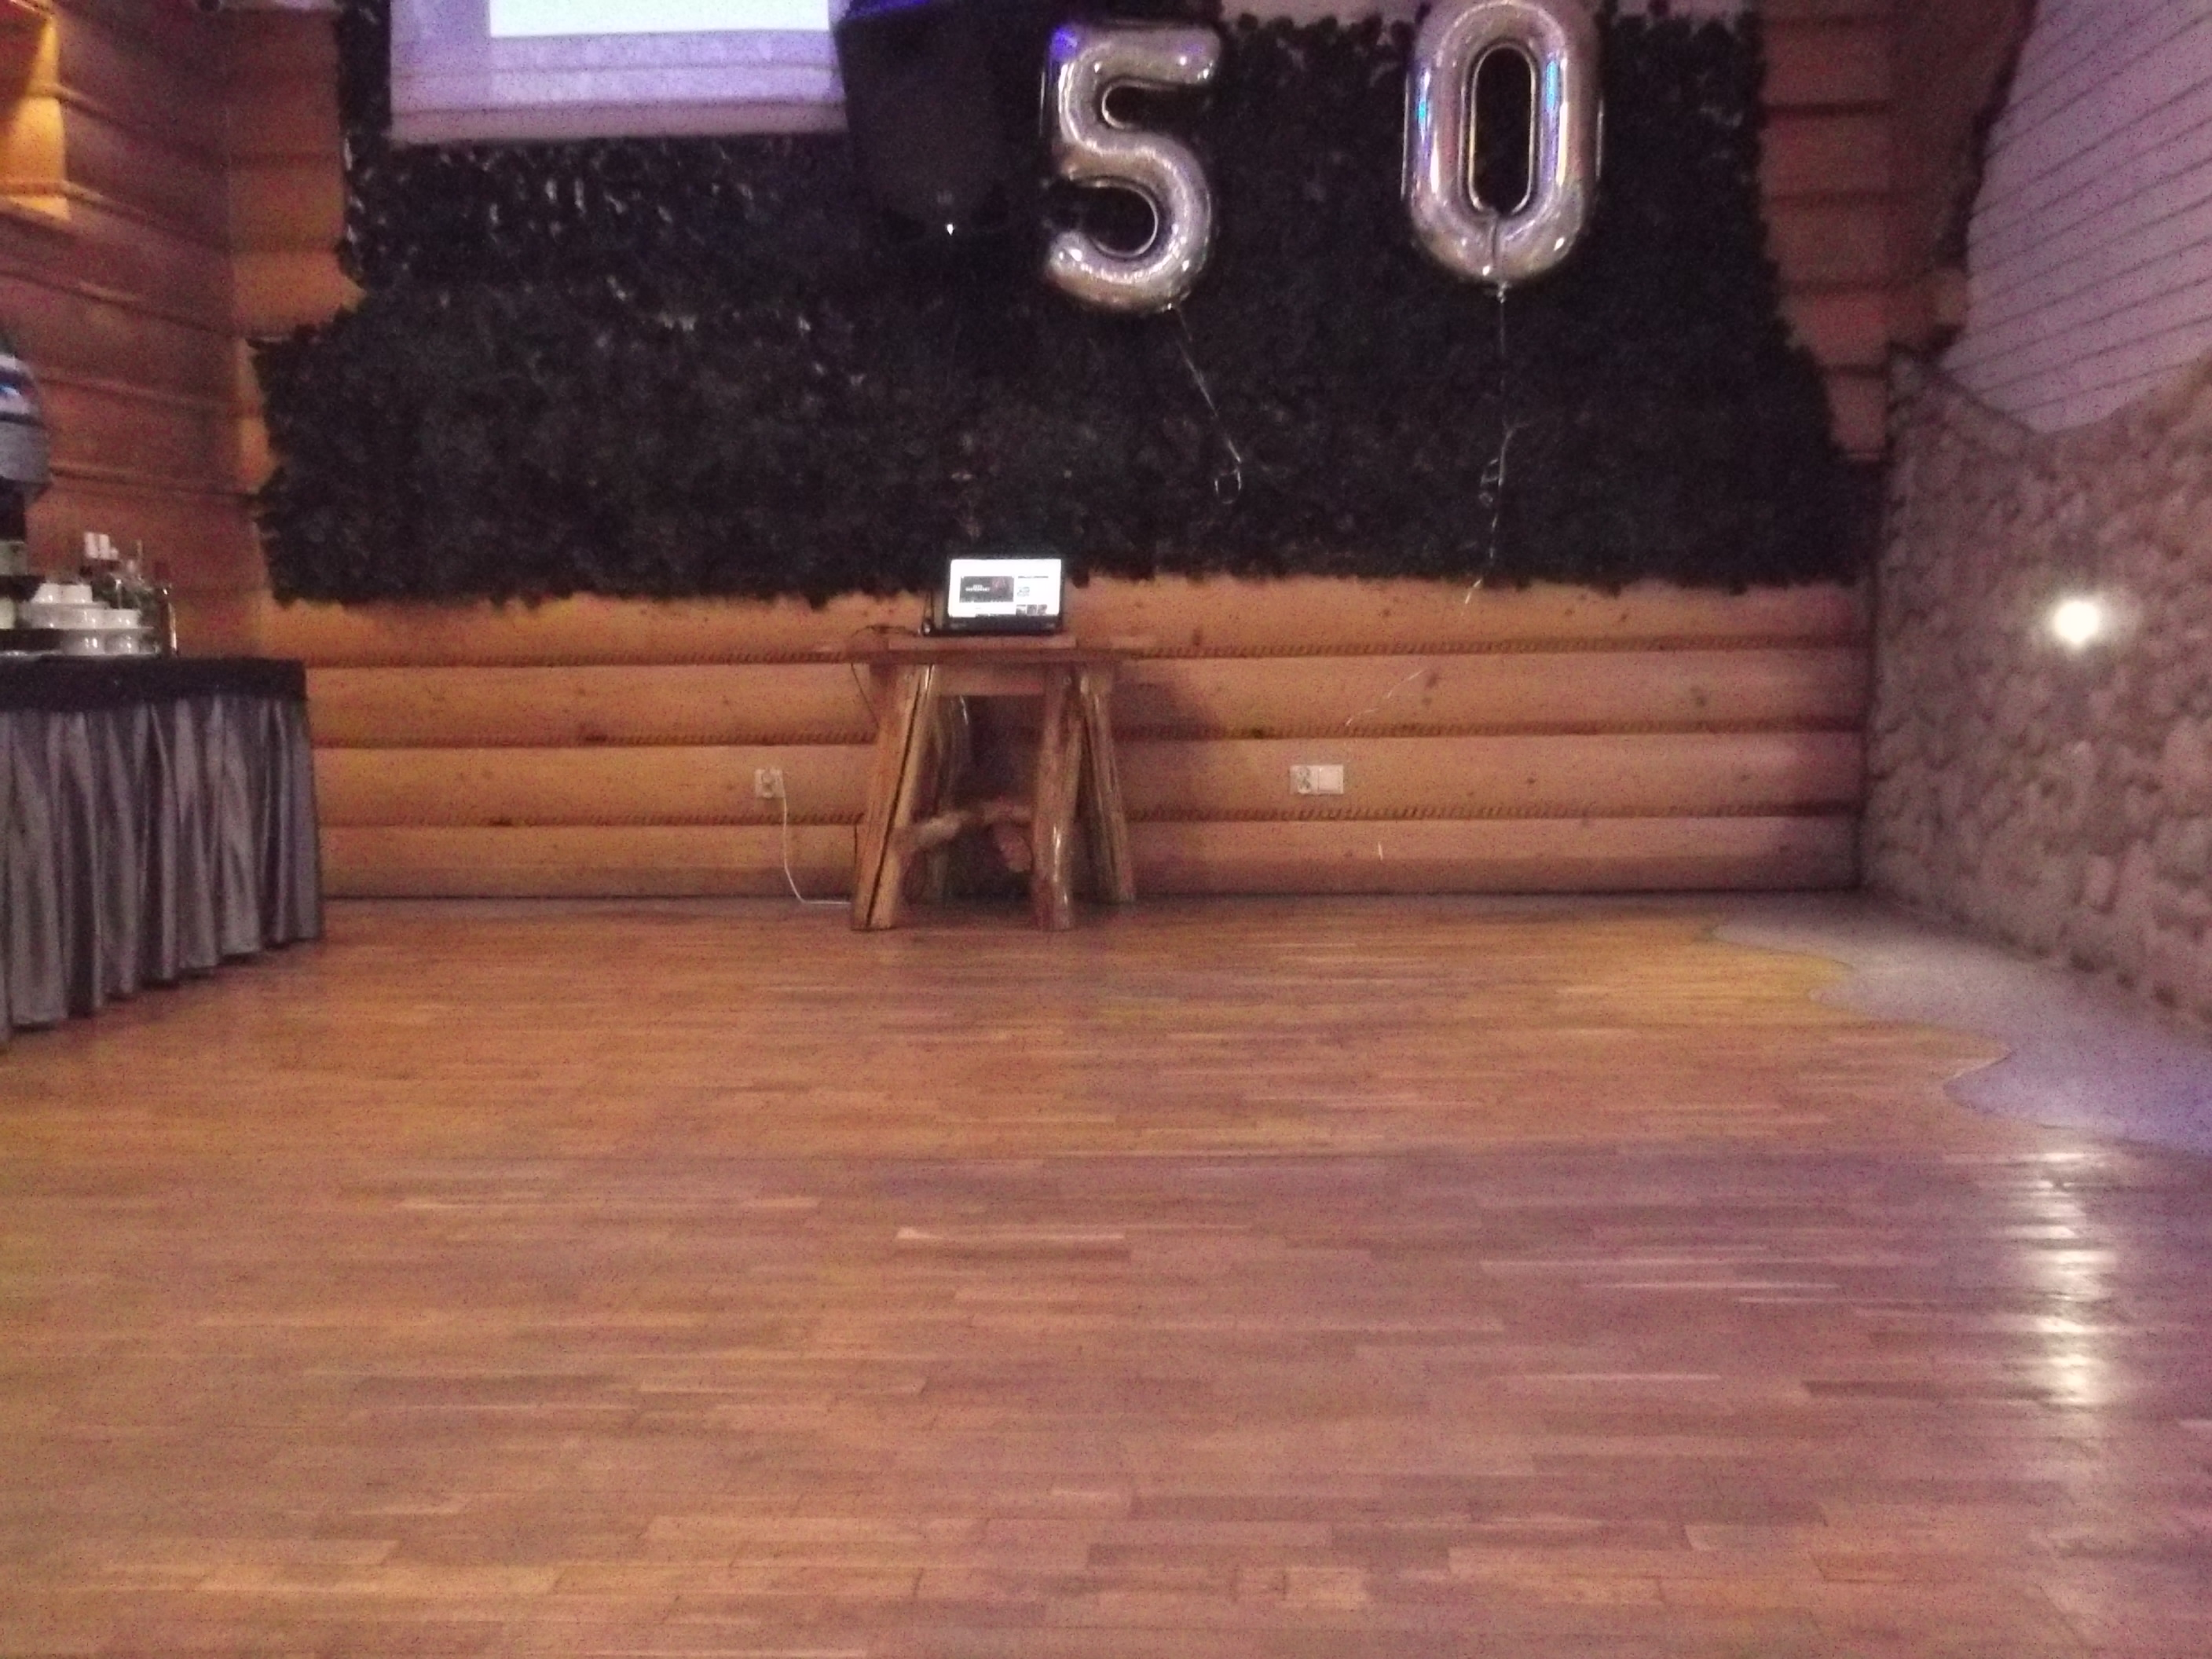
\includegraphics[width=\linewidth, keepaspectratio]{PTI_zdjęcia_i_histogramy/photos/balony3.jpg}
    \caption{Zdjęcie niedoświetlone}
\end{figure}
\begin{figure}[H]
    \centering
    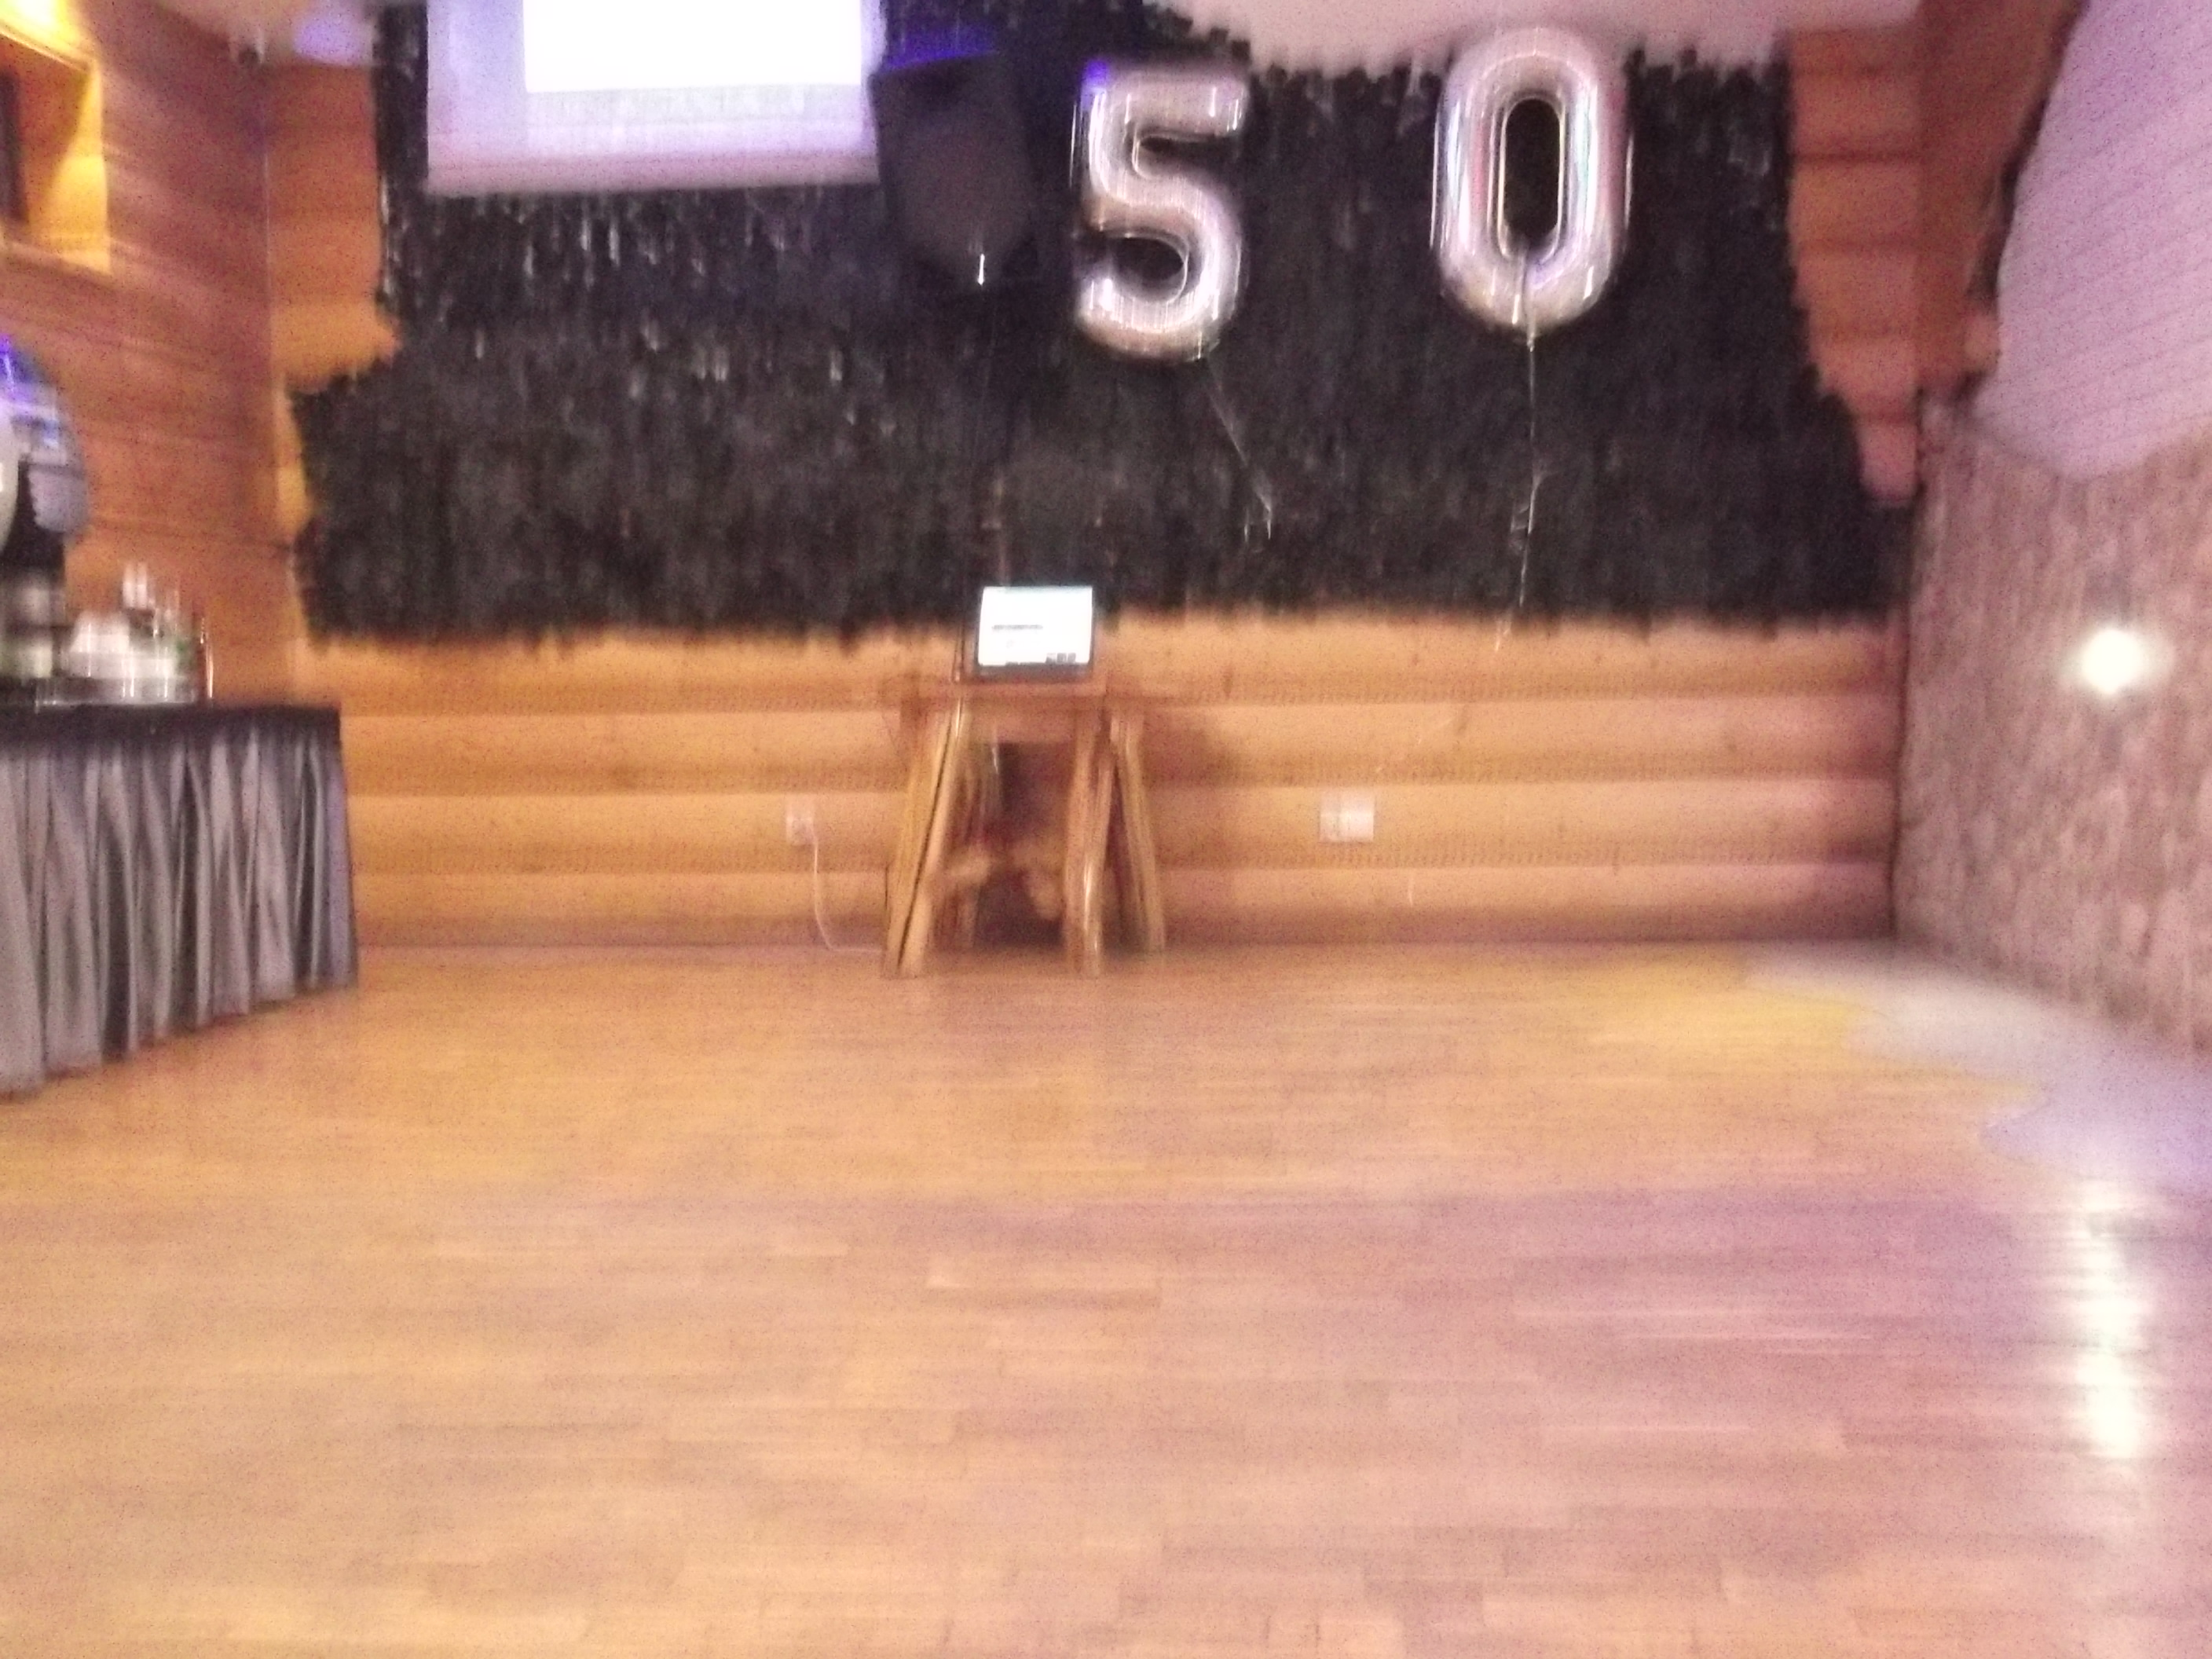
\includegraphics[width=\linewidth, keepaspectratio]{PTI_zdjęcia_i_histogramy/photos/balony2.jpg}
    \caption{Zdjęcie doświetlone}
\end{figure}
\begin{figure}[H]
    \centering
    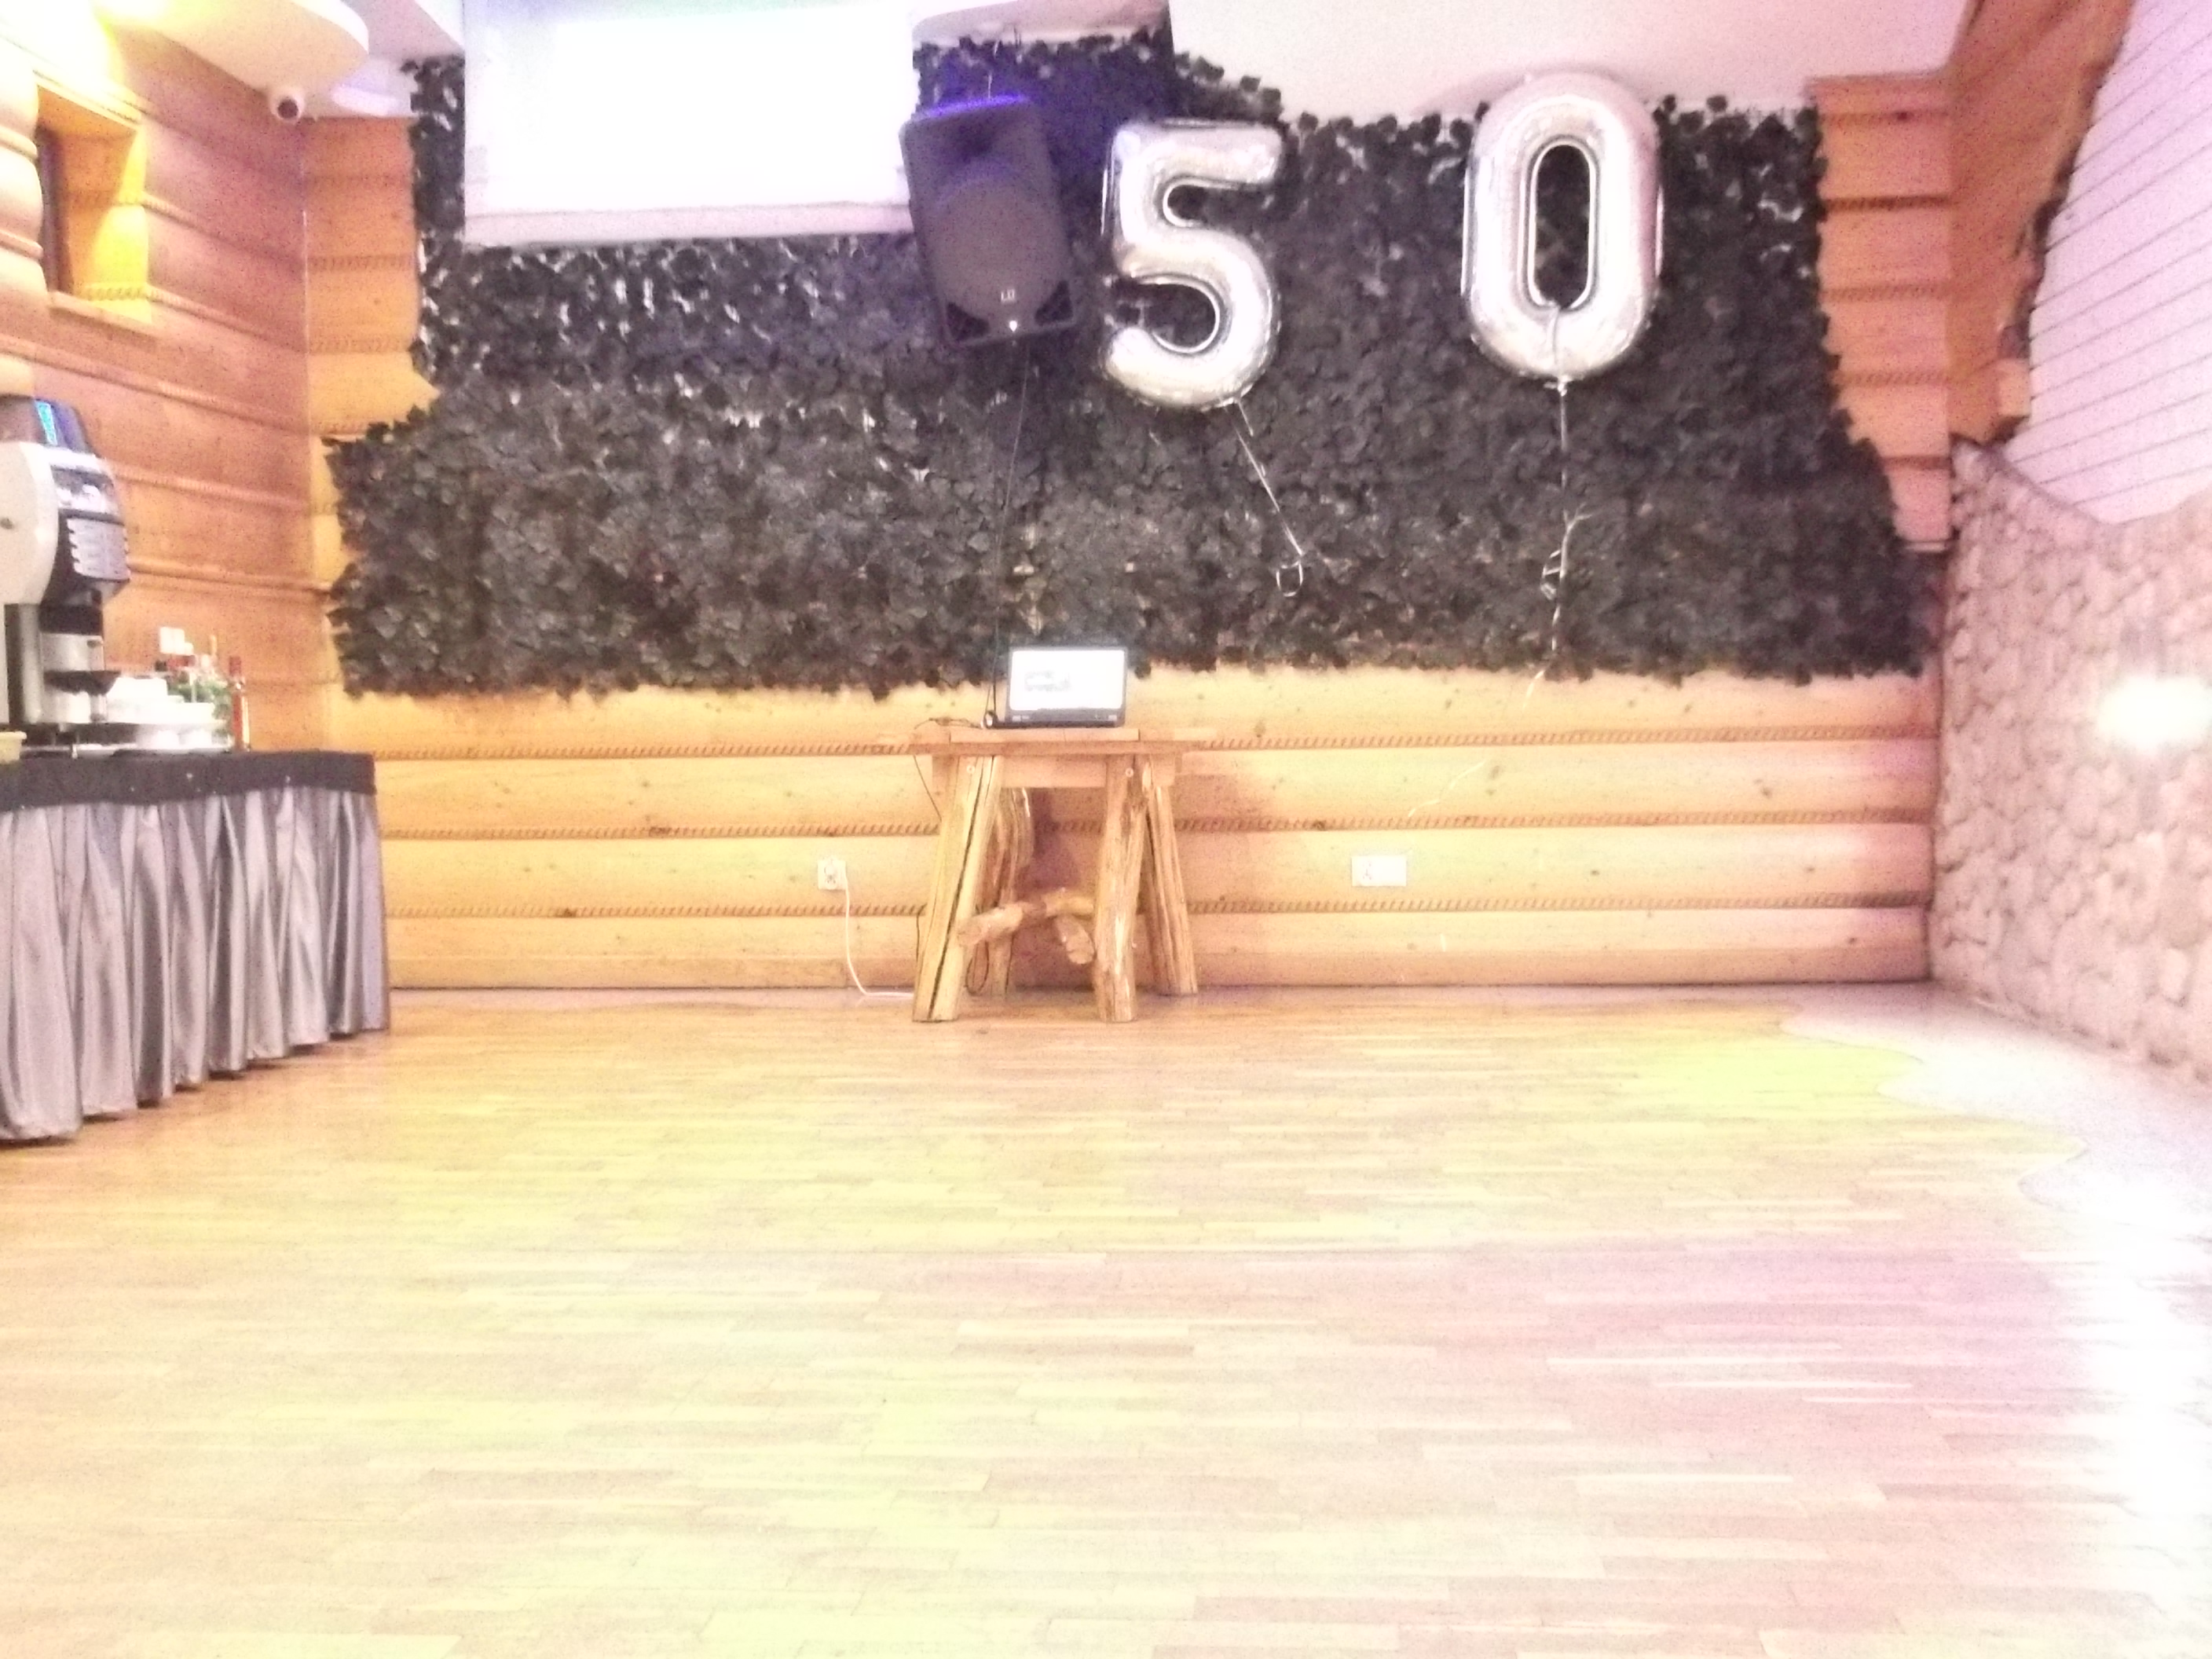
\includegraphics[width=\linewidth, keepaspectratio]{PTI_zdjęcia_i_histogramy/photos/balony1.jpg}
    \caption{Zdjęcie prześwietlone}
\end{figure}


\begin{figure}[H]
    \centering
    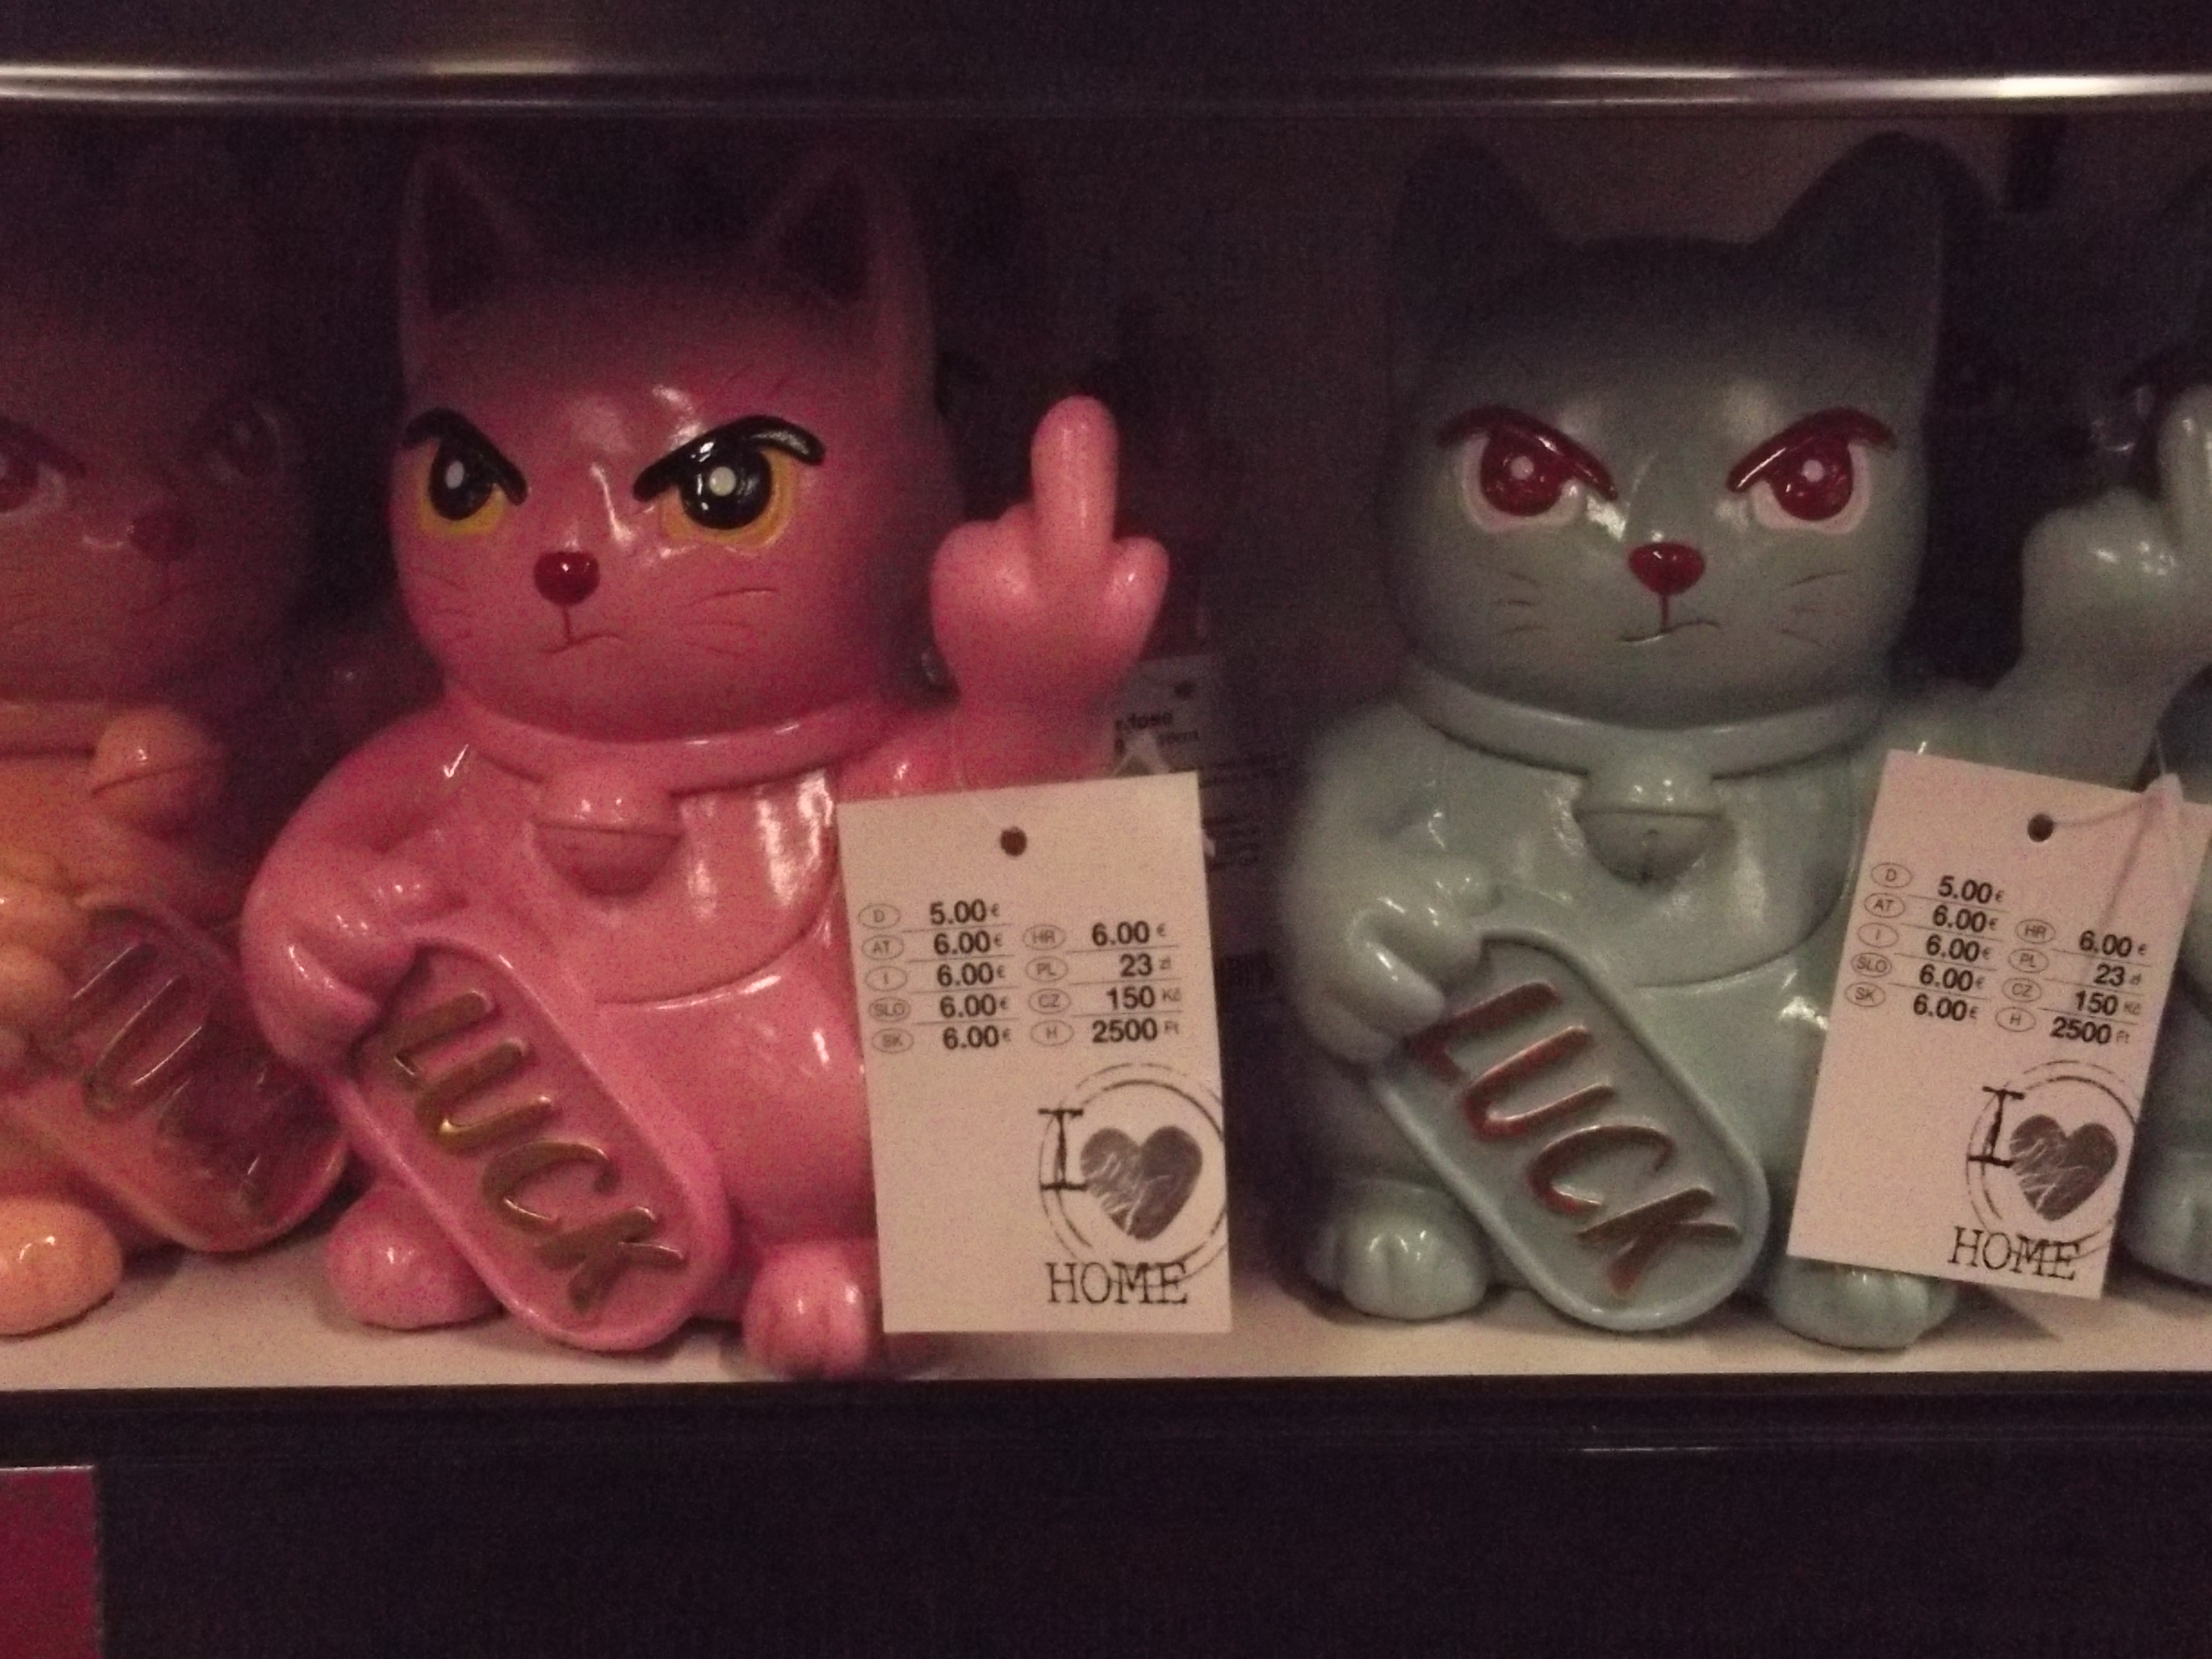
\includegraphics[width=\linewidth, keepaspectratio]{PTI_zdjęcia_i_histogramy/photos/kot3.jpg}
    \caption{Zdjęcie niedoświetlone}
\end{figure}
\begin{figure}[H]
    \centering
    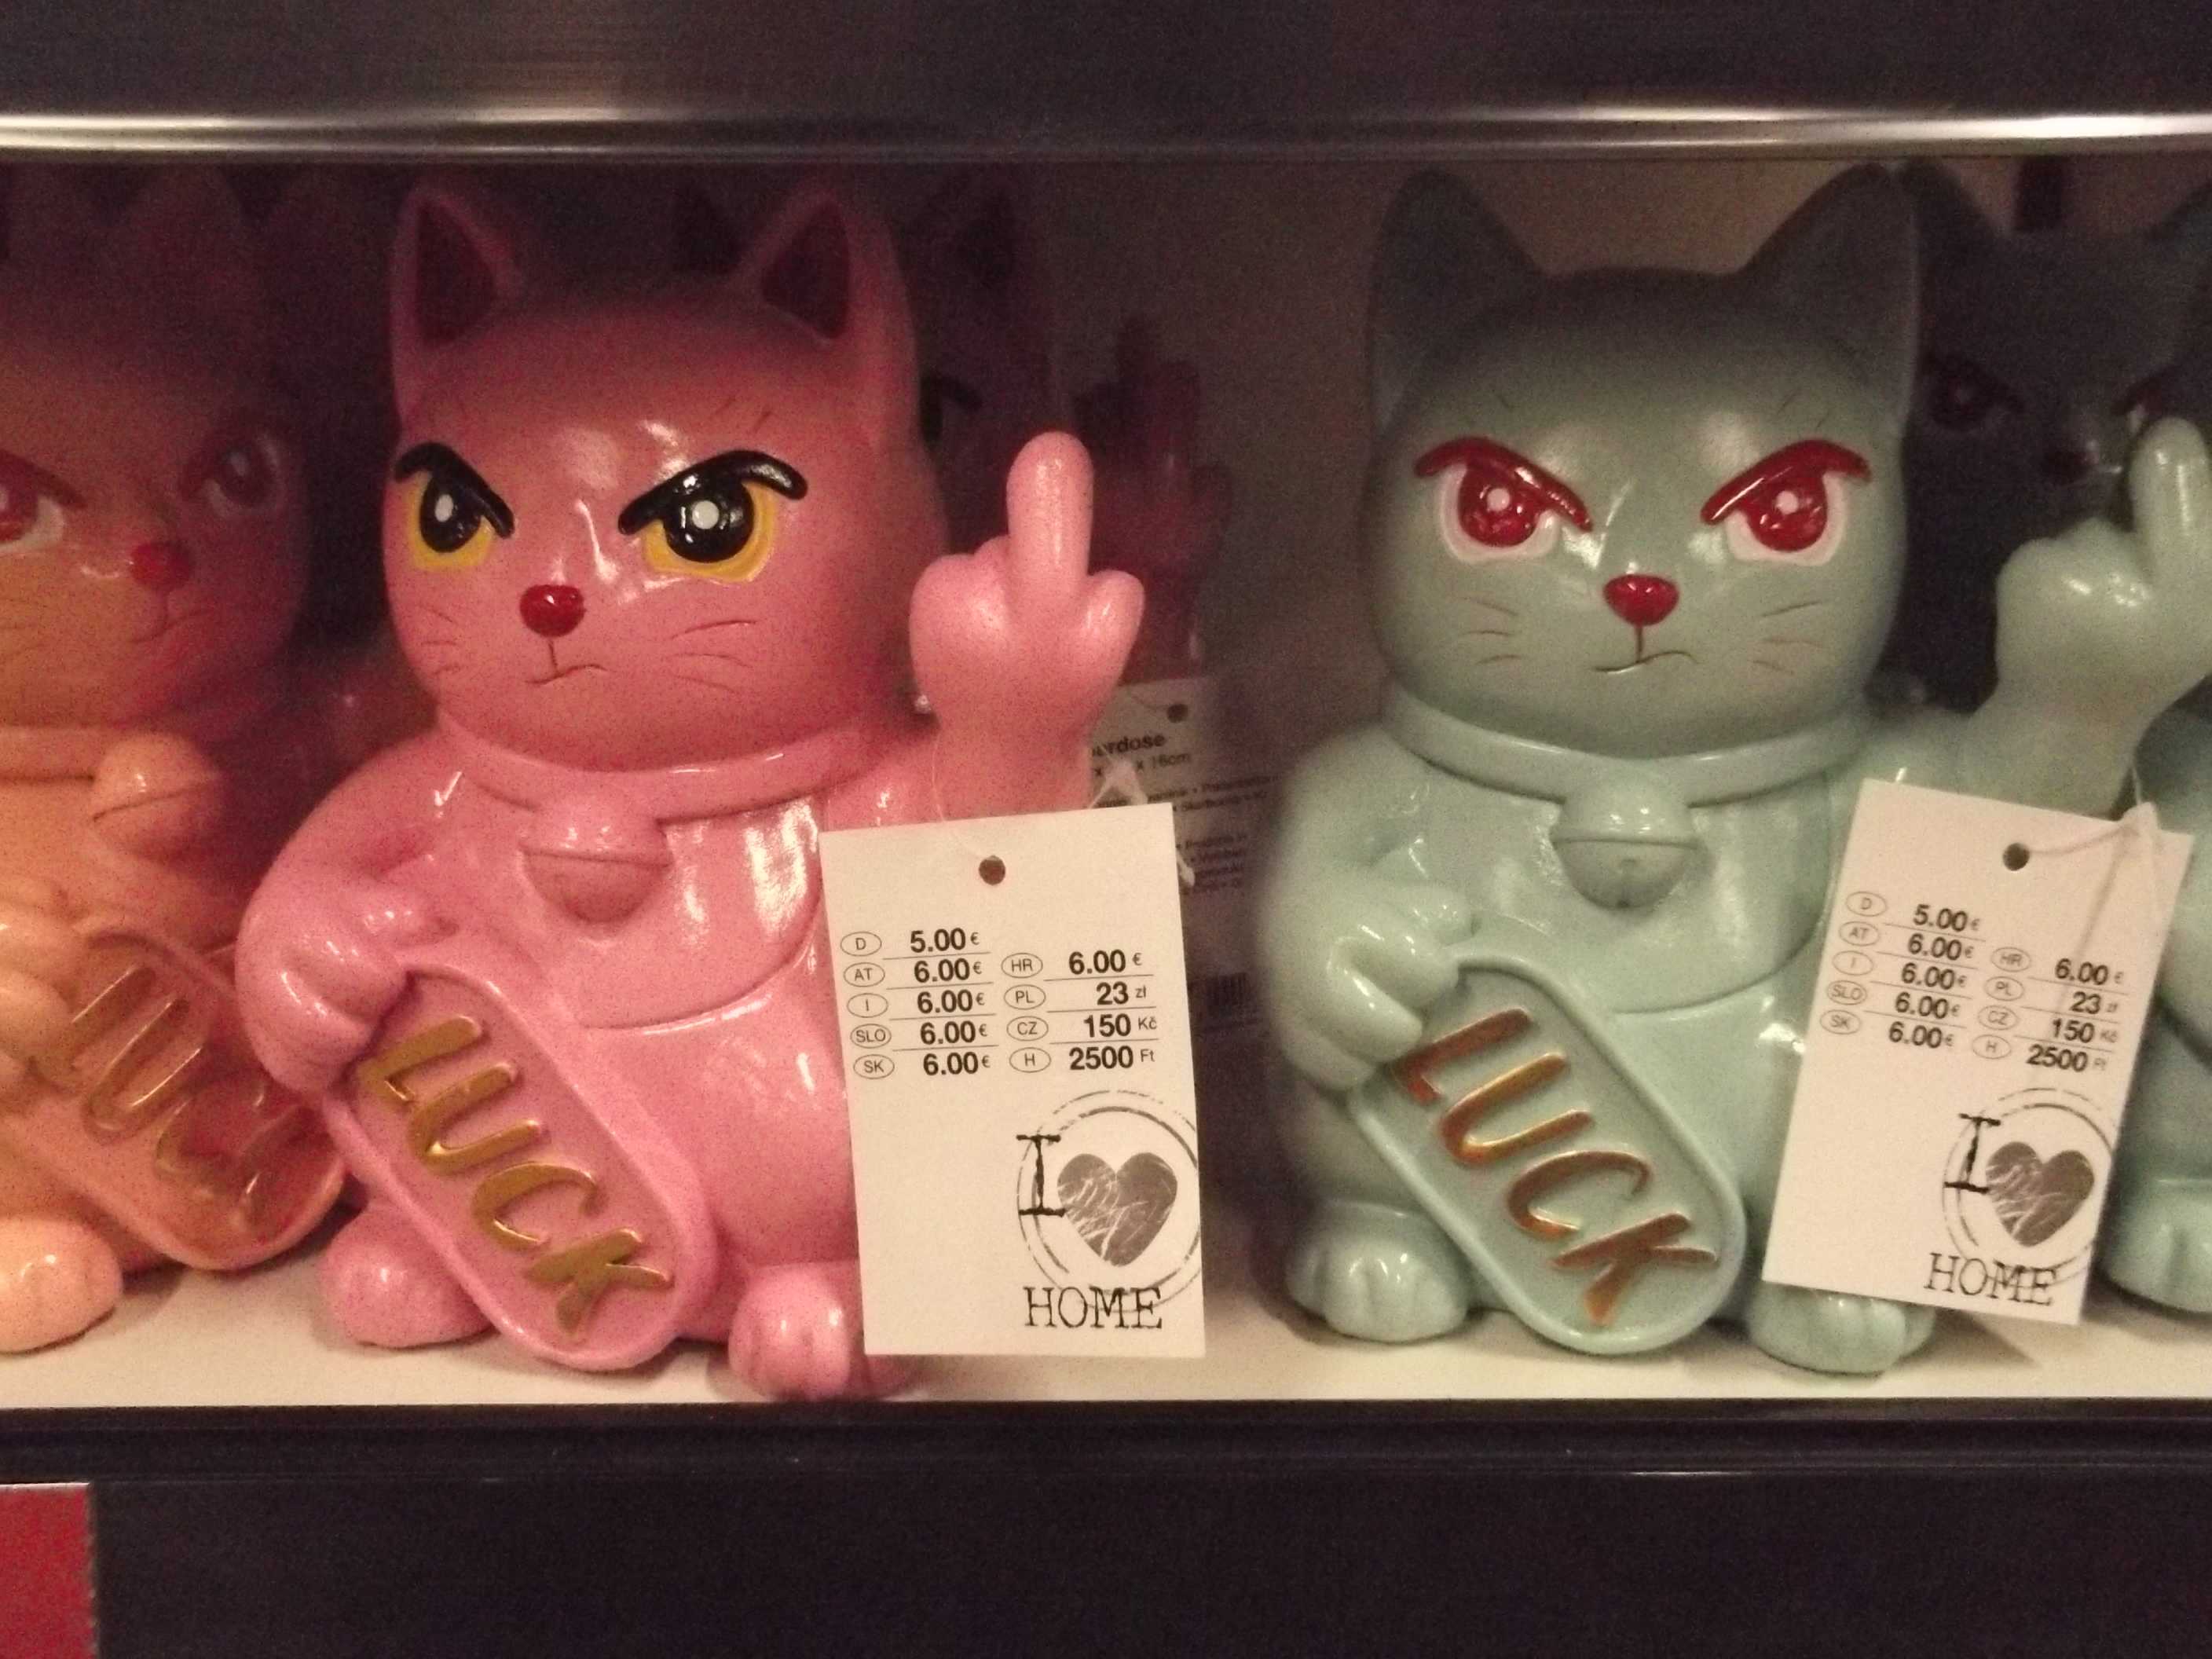
\includegraphics[width=\linewidth, keepaspectratio]{PTI_zdjęcia_i_histogramy/photos/kot2.jpg}
    \caption{Zdjęcie doświetlone}
\end{figure}
\begin{figure}[H]
    \centering
    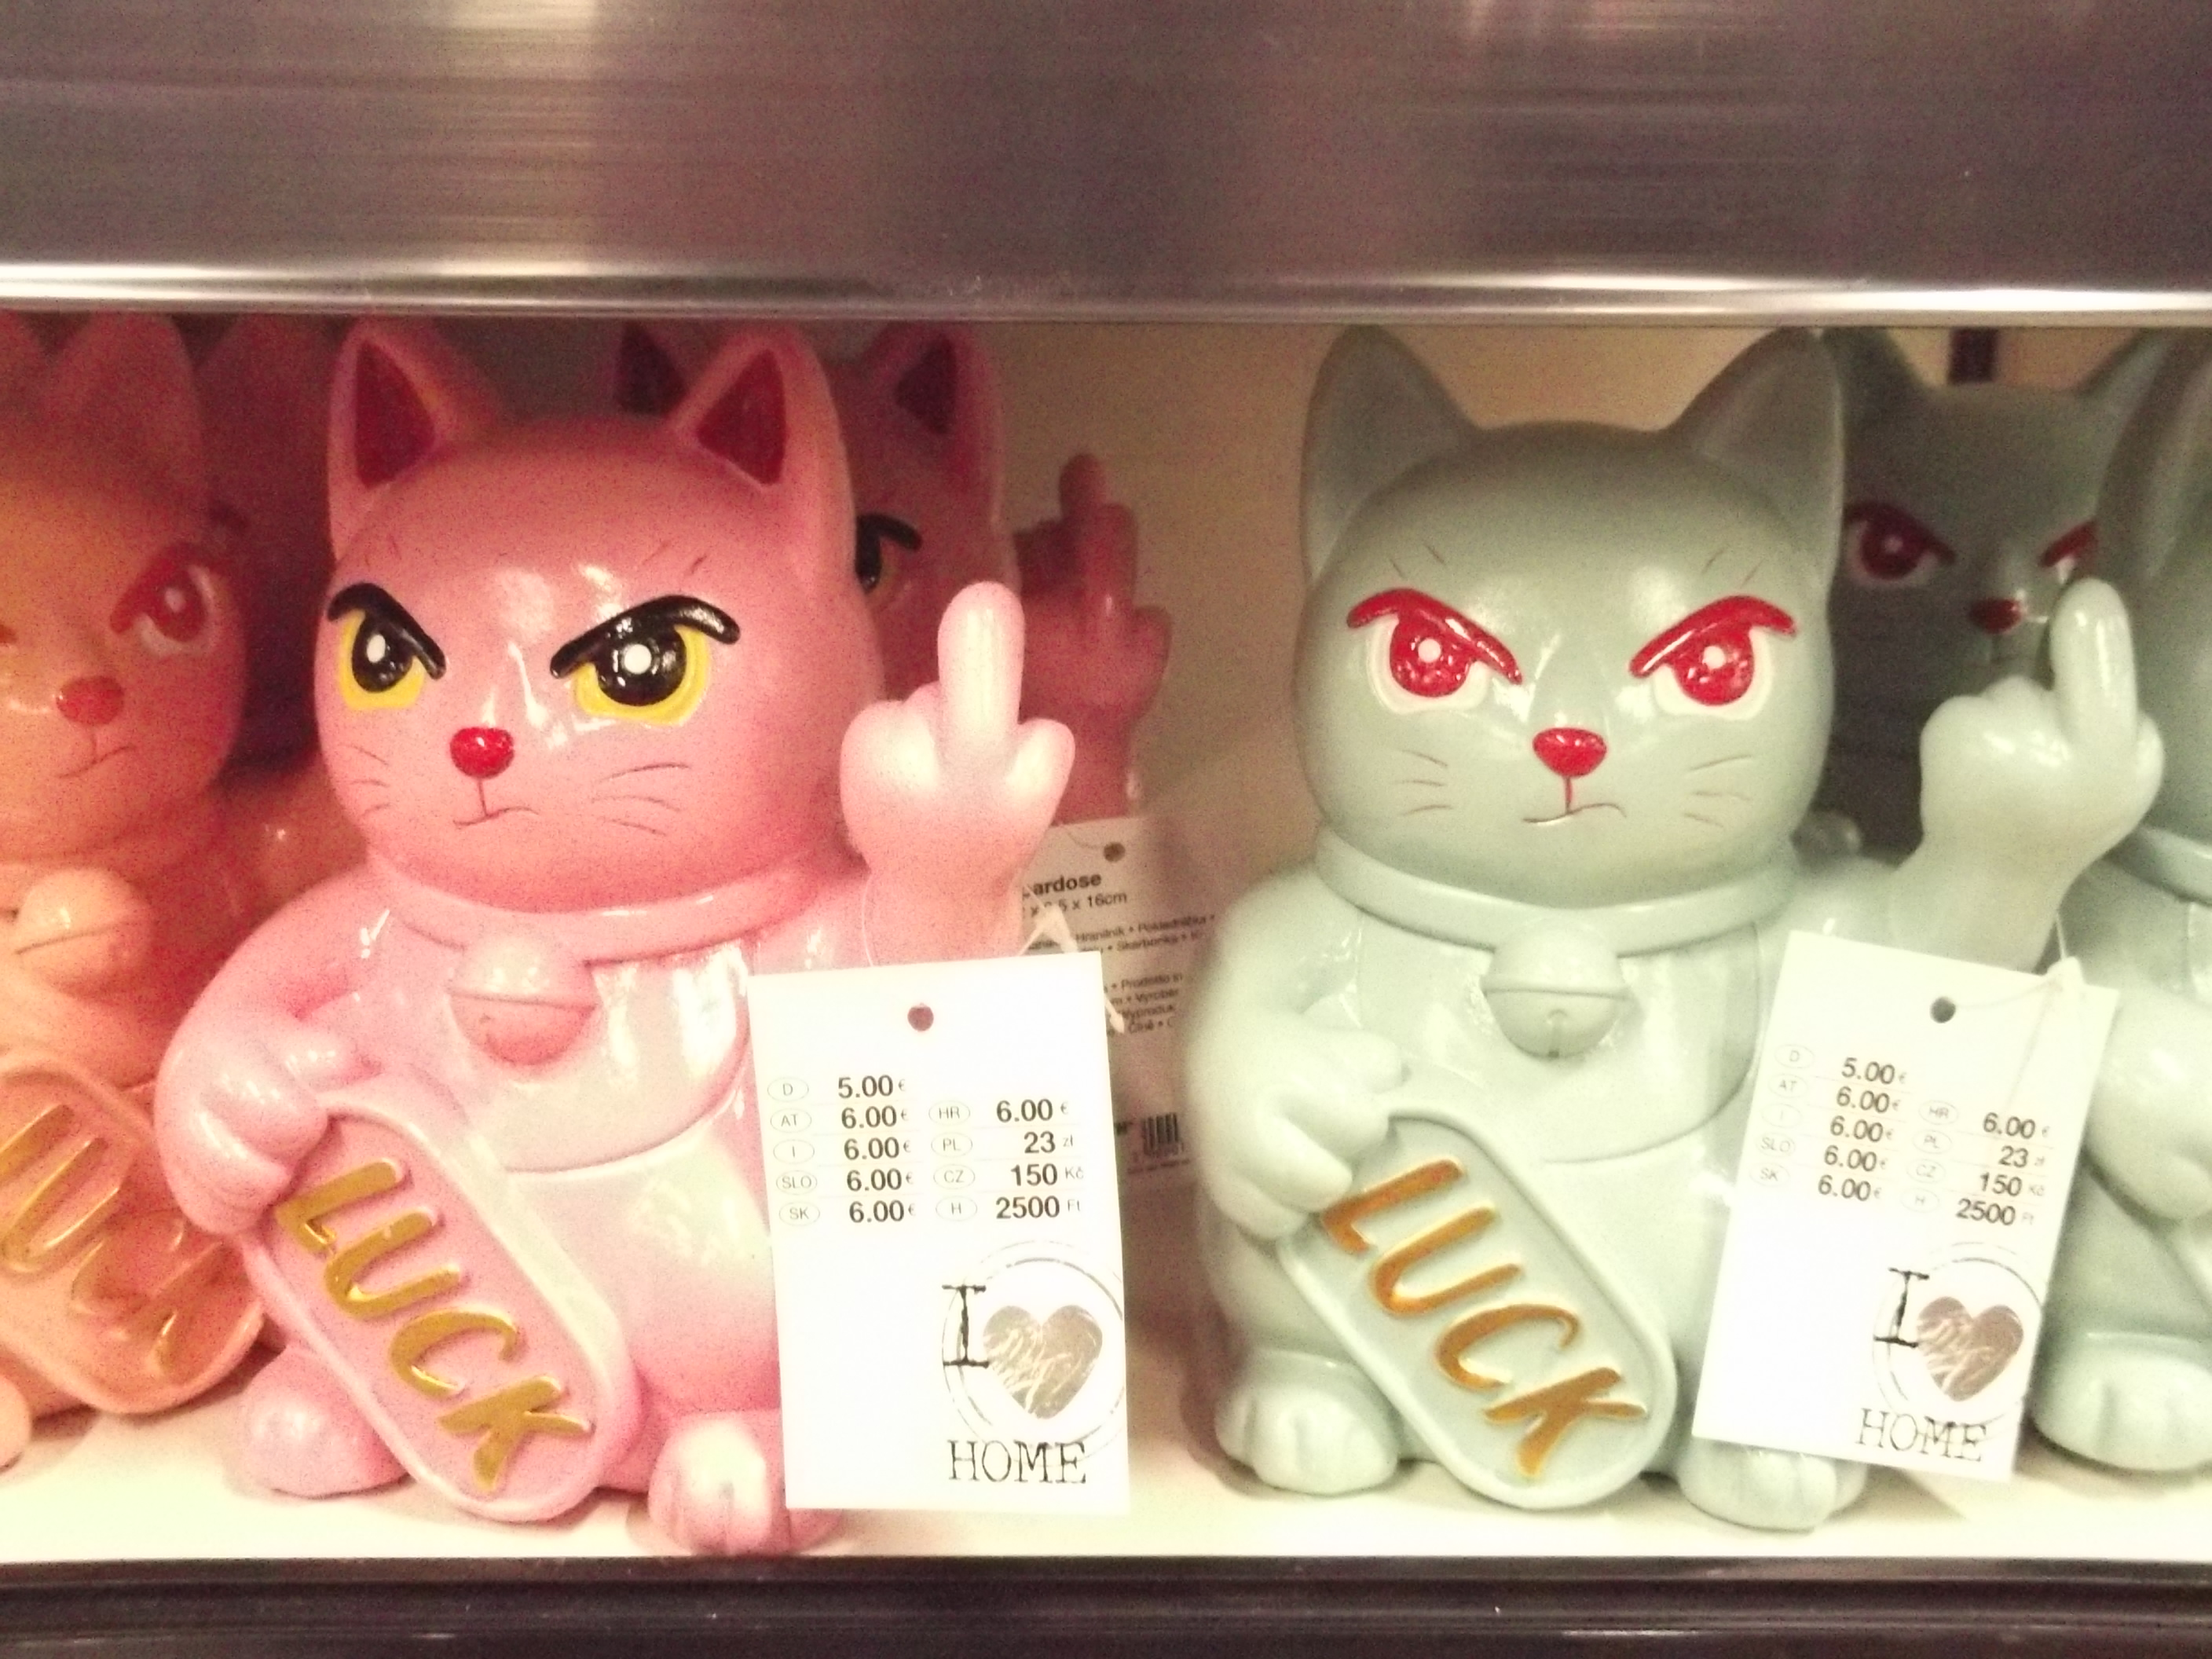
\includegraphics[width=\linewidth, keepaspectratio]{PTI_zdjęcia_i_histogramy/photos/kot1.jpg}
    \caption{Zdjęcie prześwietlone}
\end{figure}

\begin{figure}[H]
    \centering
    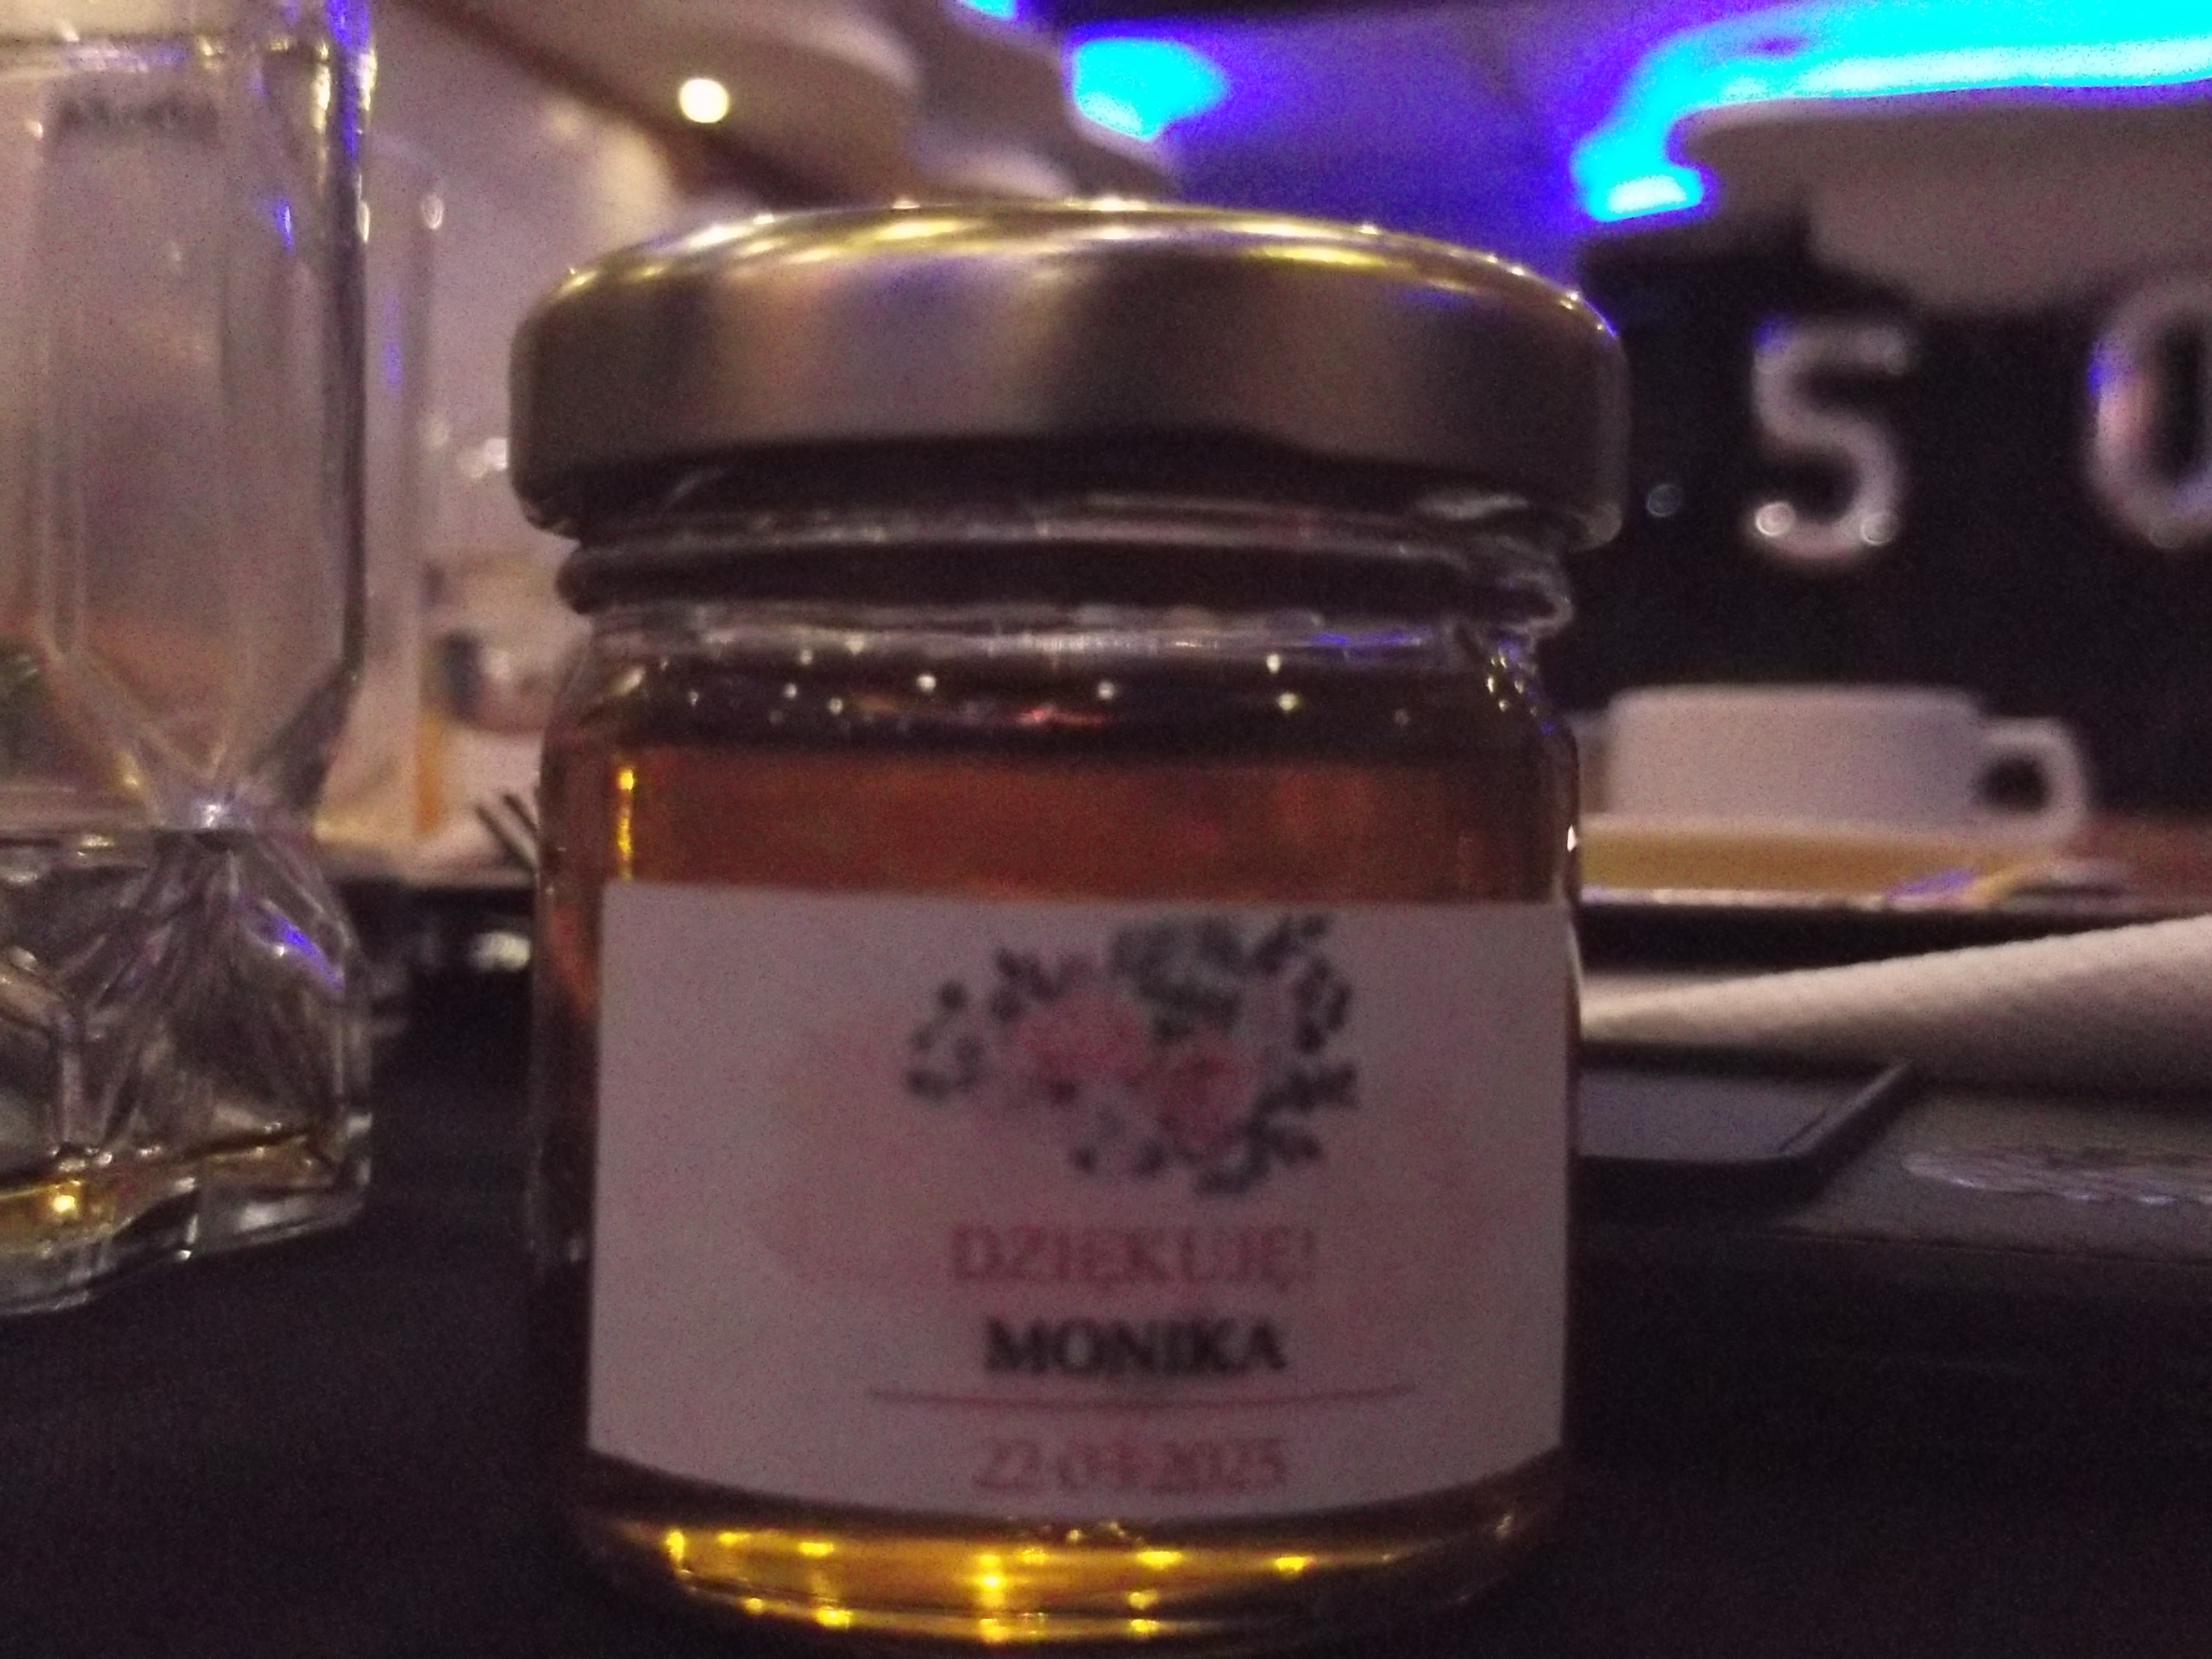
\includegraphics[width=\linewidth, keepaspectratio]{PTI_zdjęcia_i_histogramy/photos/miod3.jpg}
    \caption{Zdjęcie niedoświetlone}
\end{figure}
\begin{figure}[H]
    \centering
    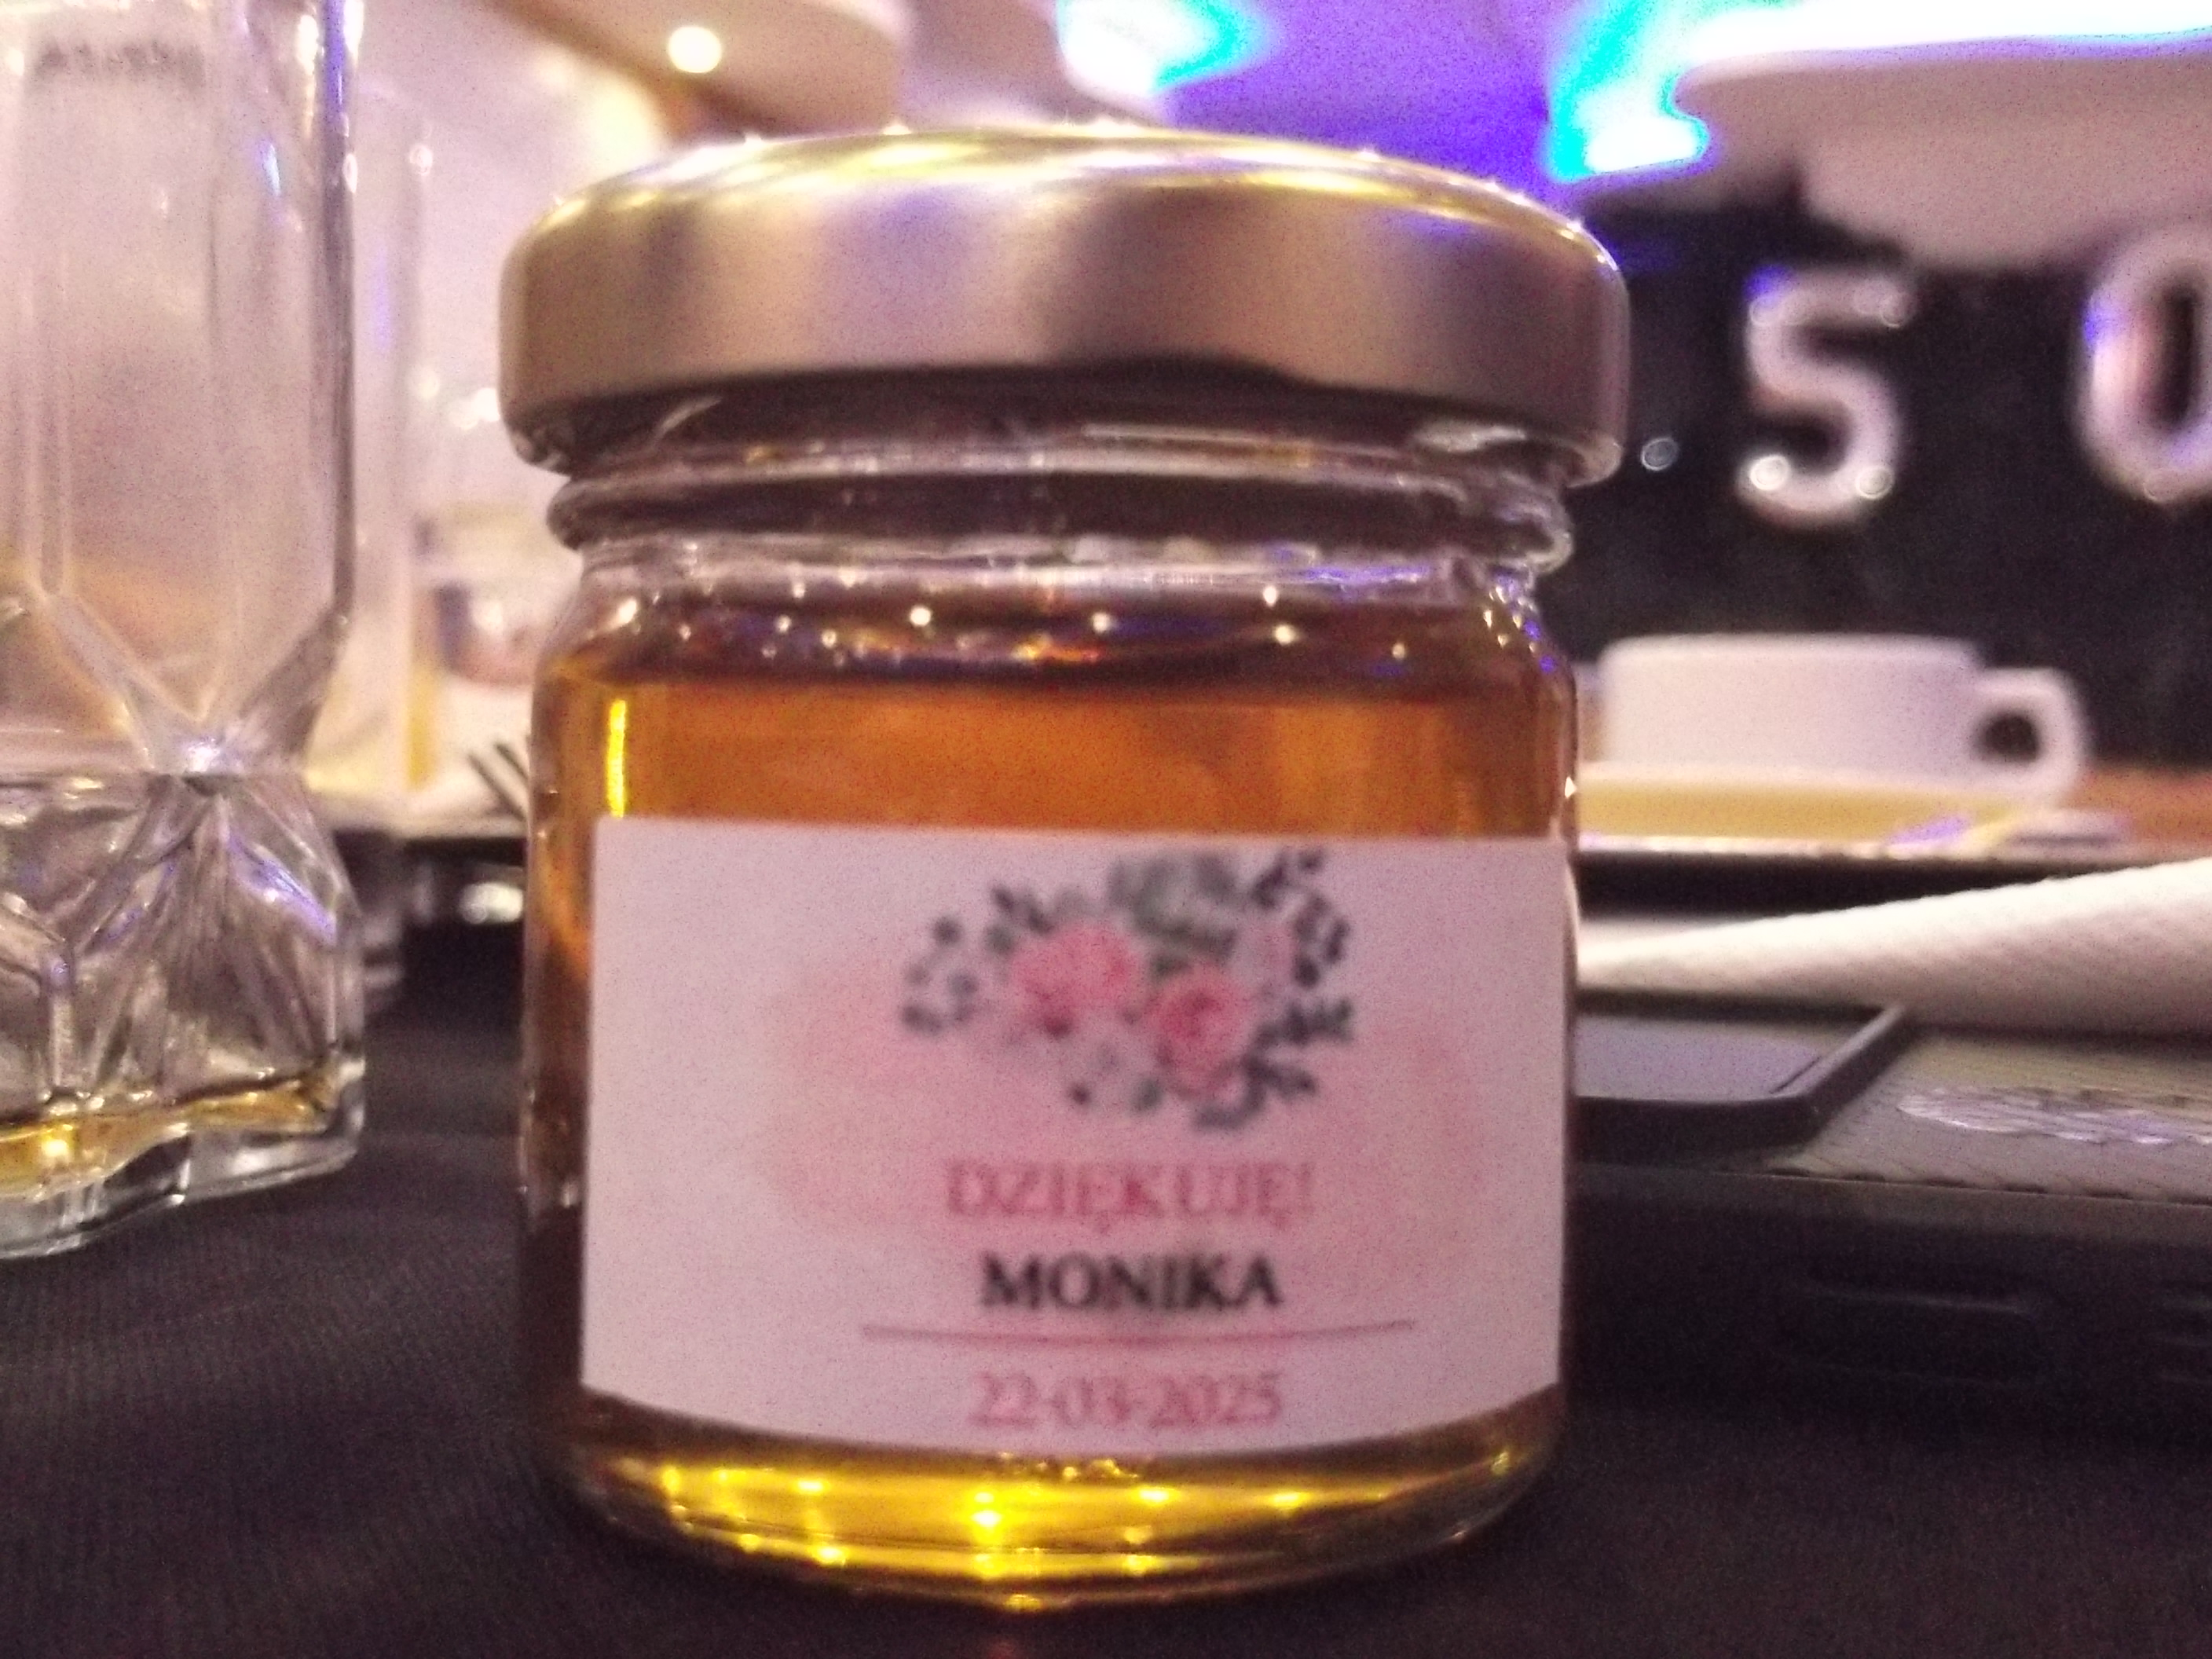
\includegraphics[width=\linewidth, keepaspectratio]{PTI_zdjęcia_i_histogramy/photos/miod1.jpg}
    \caption{Zdjęcie doświetlone}
\end{figure}
\begin{figure}[H]
    \centering
    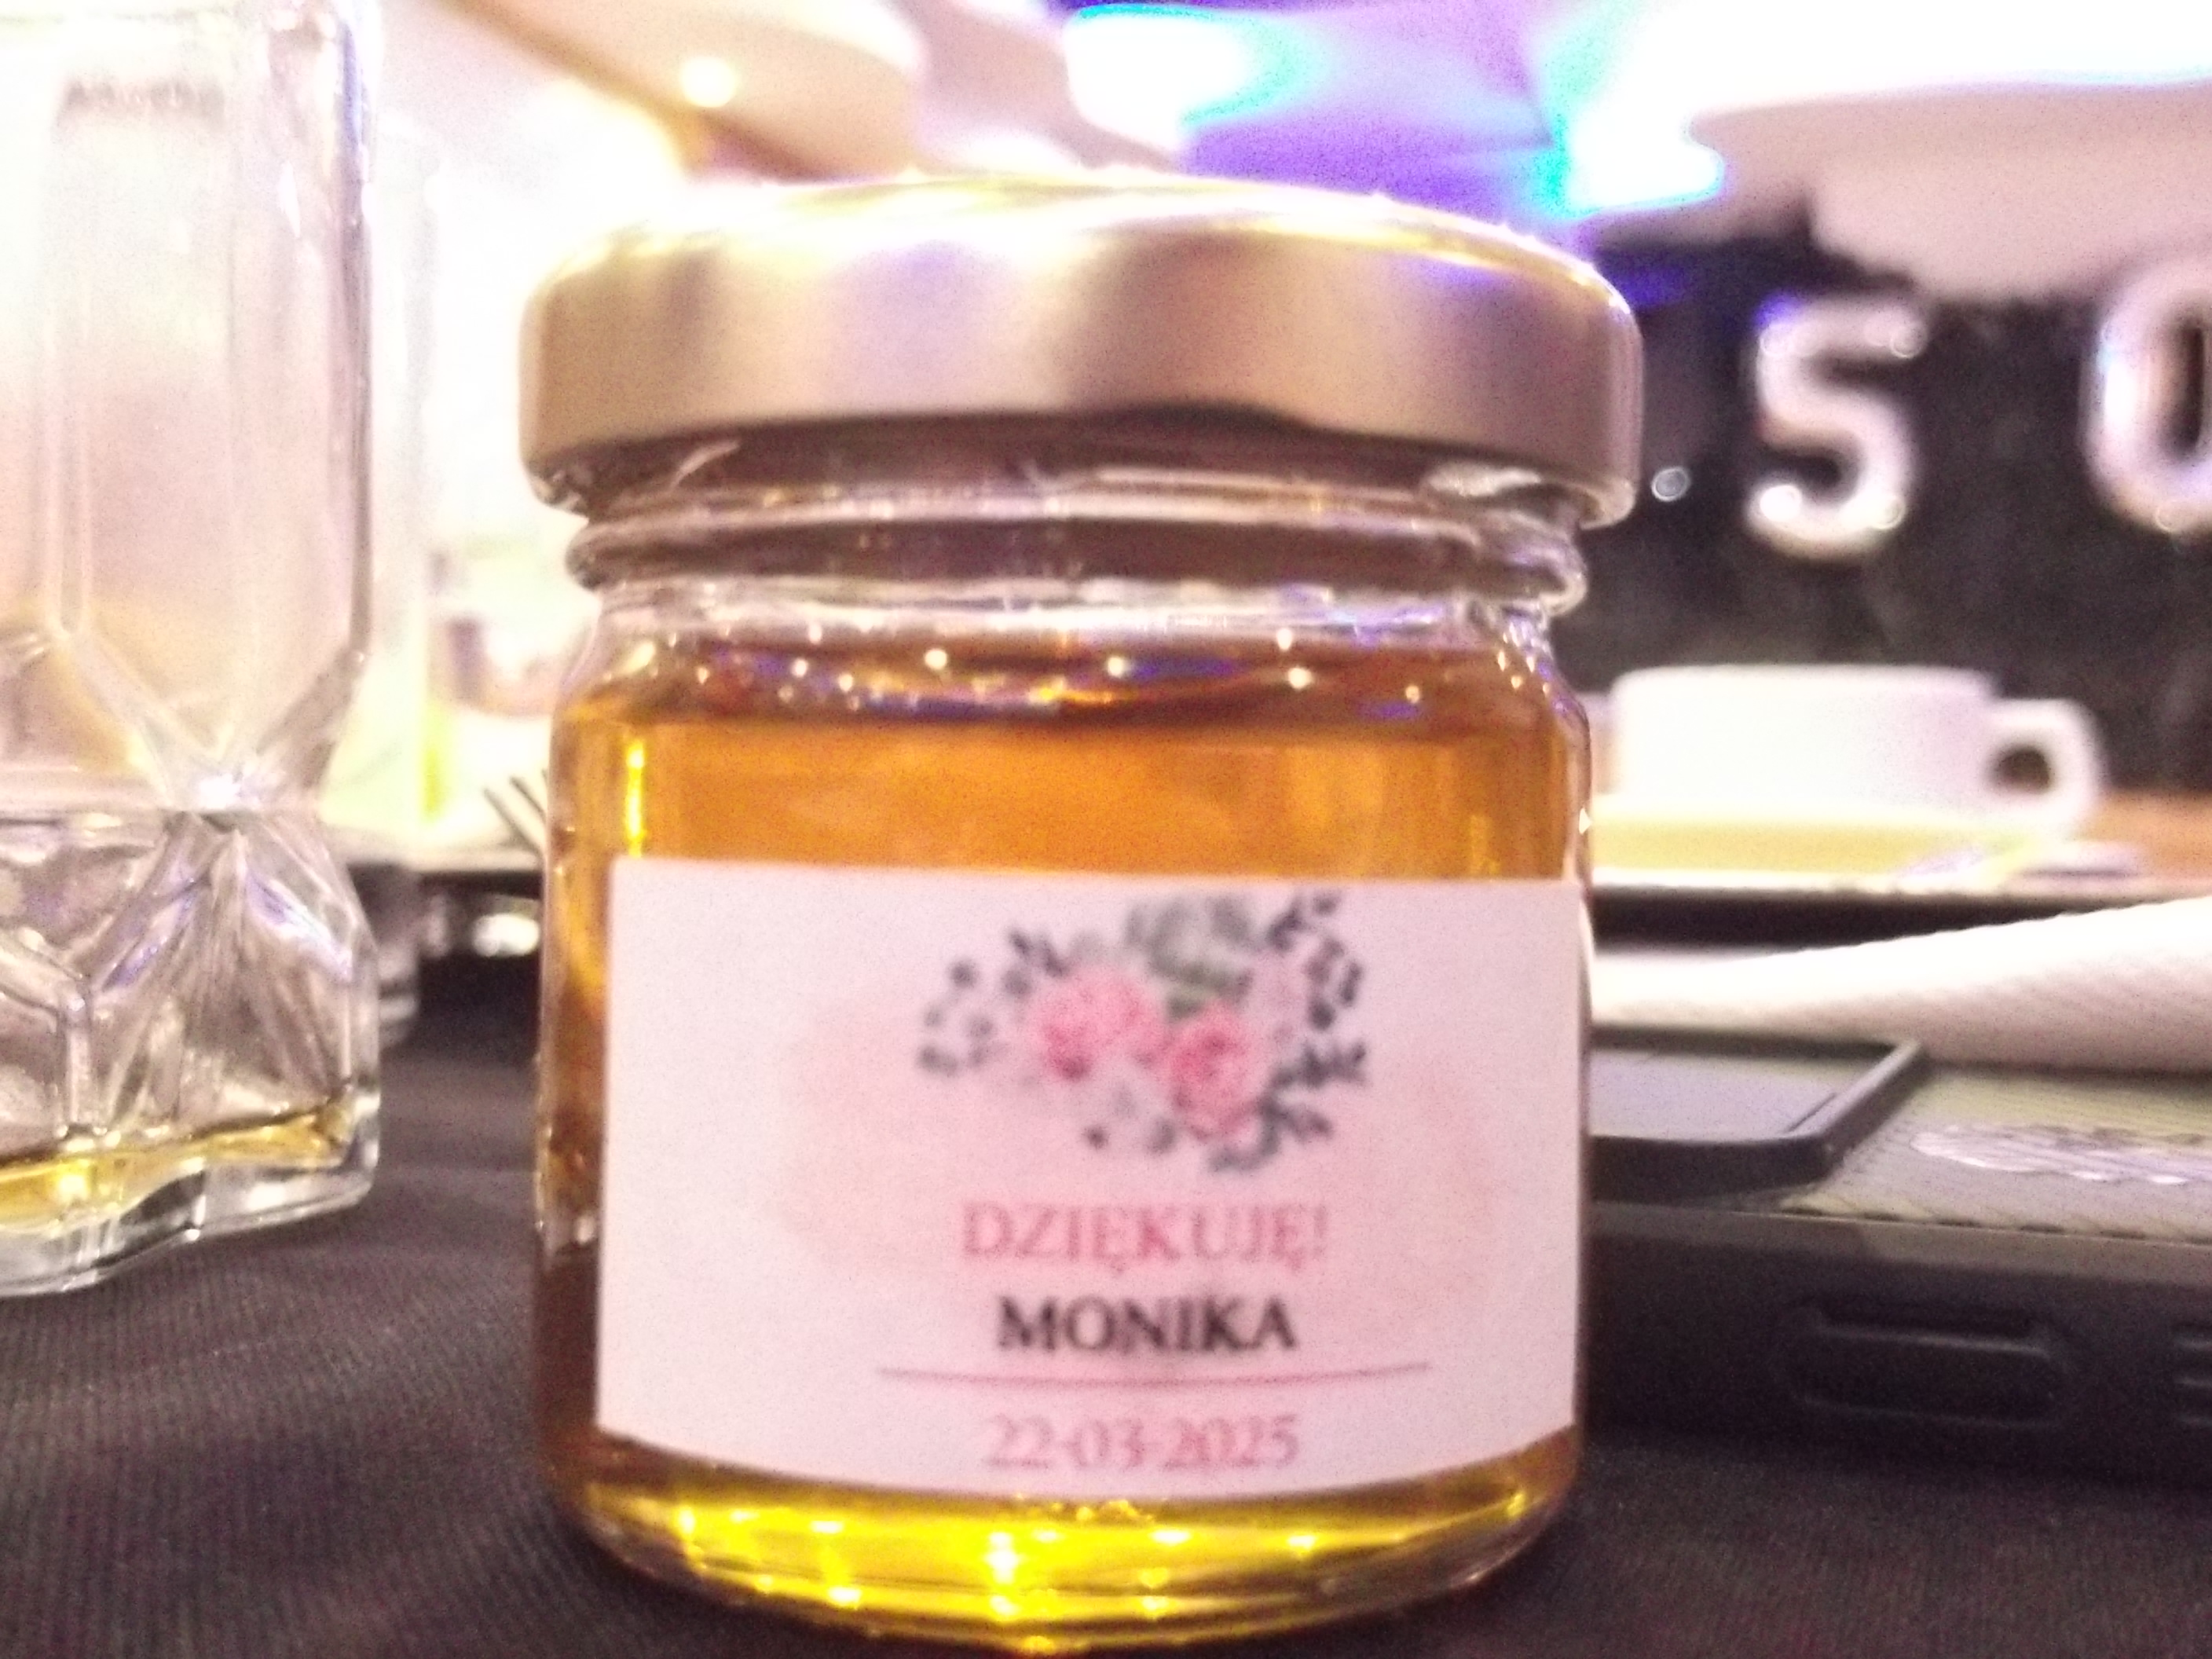
\includegraphics[width=\linewidth, keepaspectratio]{PTI_zdjęcia_i_histogramy/photos/miod2.jpg}
    \caption{Zdjęcie prześwietlone}
\end{figure}


Spora (i ciągle rosnąca) baza zdjęć analogowych i cyfrowych dogłębnie ilustrujących
sedno problemu z którym się zmagamy znajduje się tutaj:
\url{https://drive.google.com/drive/folders/1SFu_A46nBXhL19diXnxV-iyEyH0fnhFA}








\section{Wstępna analiza}
Jakkolwiek często `na oko' względnie łatwo porównując dwa zdjęcia wskazać
to, któremu brakuje szczegółów lub zostało niedoświetlone, to warto się
zastanowić co tak właściwie znaczy to, że zdjęcie jest niedoświetlone. \newline

W celu analizy i próby zdefiniowania zdjęcia o skrajnej jasności
utworzyliśmy kilka Matlabowych skryptów, które analizują wybrane
parametry zdjęć. \newline

\textit{(Uwaga techniczna) W samym raporcie posługujemy się przykładem
    kilku ujęć jednego zdjęcia aby zademonstrować nasze działania, a także
    aby zachować czytelność. Całość dostępna jest tutaj: \url{https://drive.google.com/drive/folders/1SFu_A46nBXhL19diXnxV-iyEyH0fnhFA}.}


\newpage
\subsection{Intensywność}
W przypadku analizy zdjęcia intensywność odnosi się do jasności piksela i
opisuje ogólną ilość światła w obrazie. Jest to miara luminancji, czyli składowej
jasności obrazu, niezależna od koloru. Utworzyliśmy histogramy pokazujące rozłożenie
jasności pikseli na obrazach. Na podstawie tych wykresów można wysunąć wnioski na
temat tego czy zdjęcie jest dobrze oświetlone, niedoświetlone czy prześwietlone.
Zauważyliśmy, że zebrane przez nas zdjęcia analogowe są znacznie ciemniejsze od
tych cyfrowych. Histogramy zdjęć robionych w tych samych warunkach, ale z inną
ekspozycją znacząco różnią się między sobą, jednak ta różnica jest najbardziej
widoczna w przypadku zdjęć cyfrowych.


\subsubsection{Kod}
\begin{verbatim}
    files = dir("photos\*.jpg");
    
    for i = 1:length(files)
    
    clear count g G im k light max n s x y;
    im = imread(strcat("photos\", files(i).name));
    g = rgb2gray(im);
    G = g(:);
    s = length(G);
    figure(1);
    set(gcf, 'Units', 'Normalized', 'OuterPosition', [0 0 1 1]); %wielkość okna
    
    
    subplot(1,3,[1,2]); 
    histogram(G,'FaceColor', '#ffffff');
    
    [count, n] = histcounts( G, 255 );
    max = max(count);
    max = max*1.2;
    
    xlim([0 255]);
    ylim([0,max]);
    
    grid on;
    title('Histogram jasności pikseli','FontSize', 30);
    xlabel('Wartość jasności','FontSize',20);
    ylabel('Ilośc pikseli','FontSize',20);
    
    x = [0 0 0 0];
    y = [0 0 max max];
    light = 0.66;
    for k =1:1:5
        hold on;
        x = x + [0 51 51 0];
        patch(x,y,'k','FaceAlpha',light);
        x = x + [51 0 0 51];
        light = light *0.66;
    end
    
    subplot(1,3,3);
    imshow(im);
    
    exportgraphics(gcf, strcat("intensity\", 
                        \\files(i).name(1:length(files(i).name)-4),"_intensity.jpg"))
    close;
    end
    \end{verbatim}


\subsubsection{Wyniki}

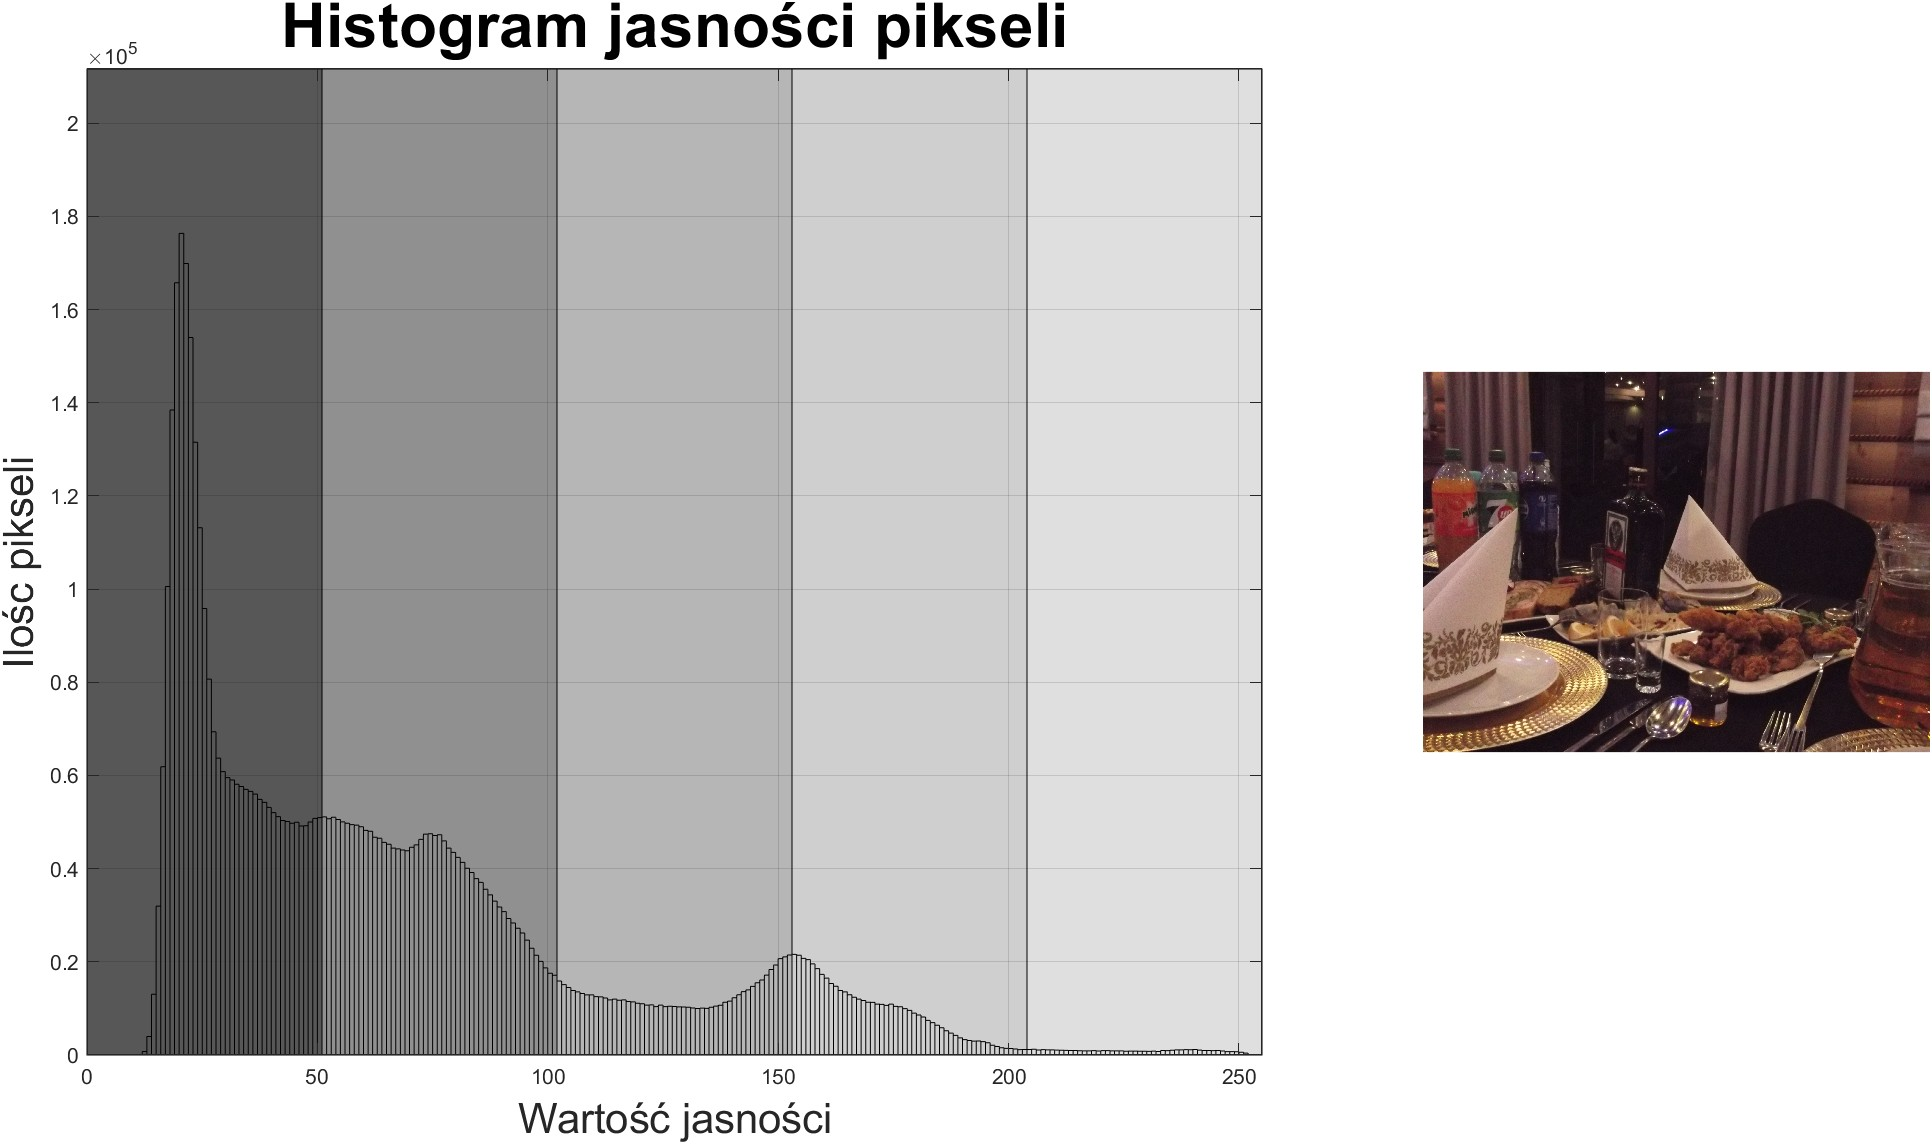
\includegraphics[width=\textwidth]{PTI_zdjęcia_i_histogramy/intensity/jagier1_intensity.jpg}
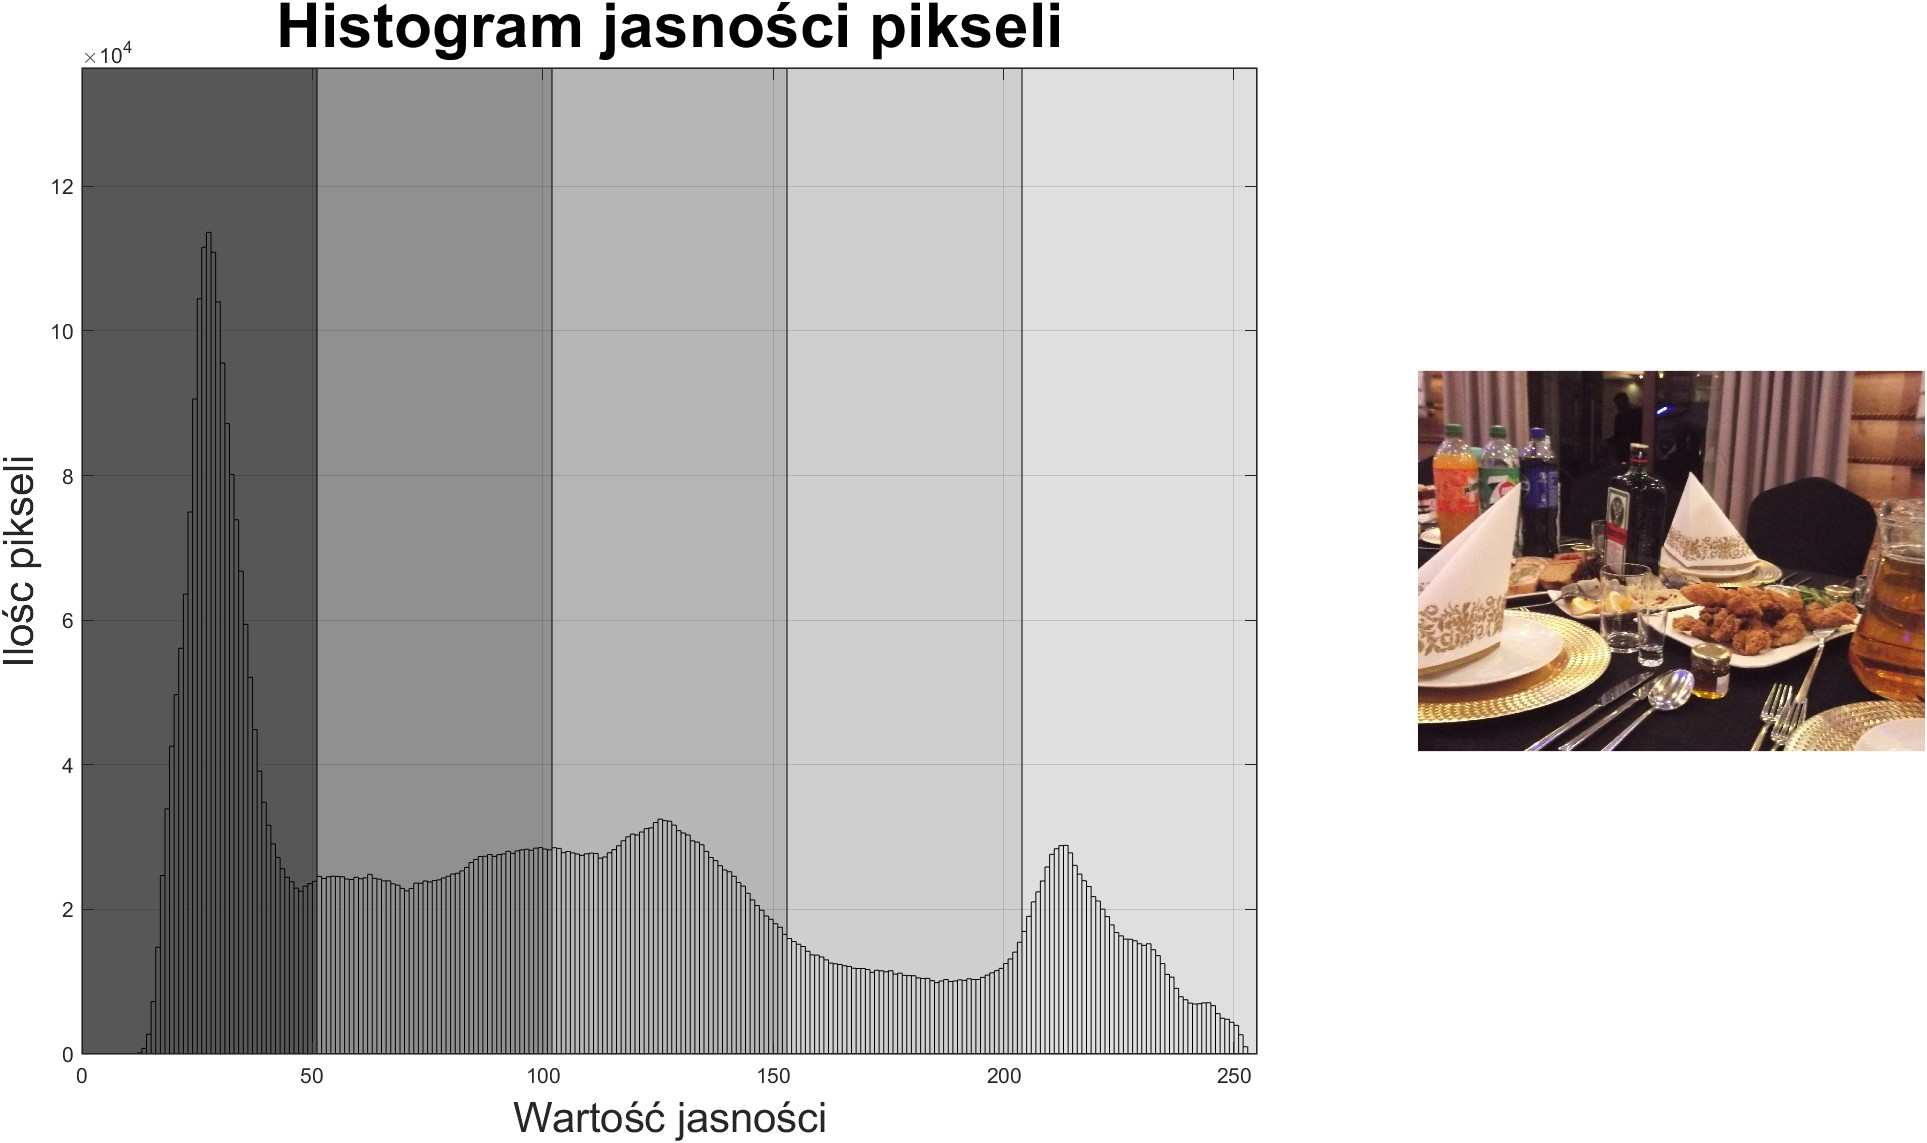
\includegraphics[width=\textwidth]{PTI_zdjęcia_i_histogramy/intensity/jagier2_intensity.jpg}
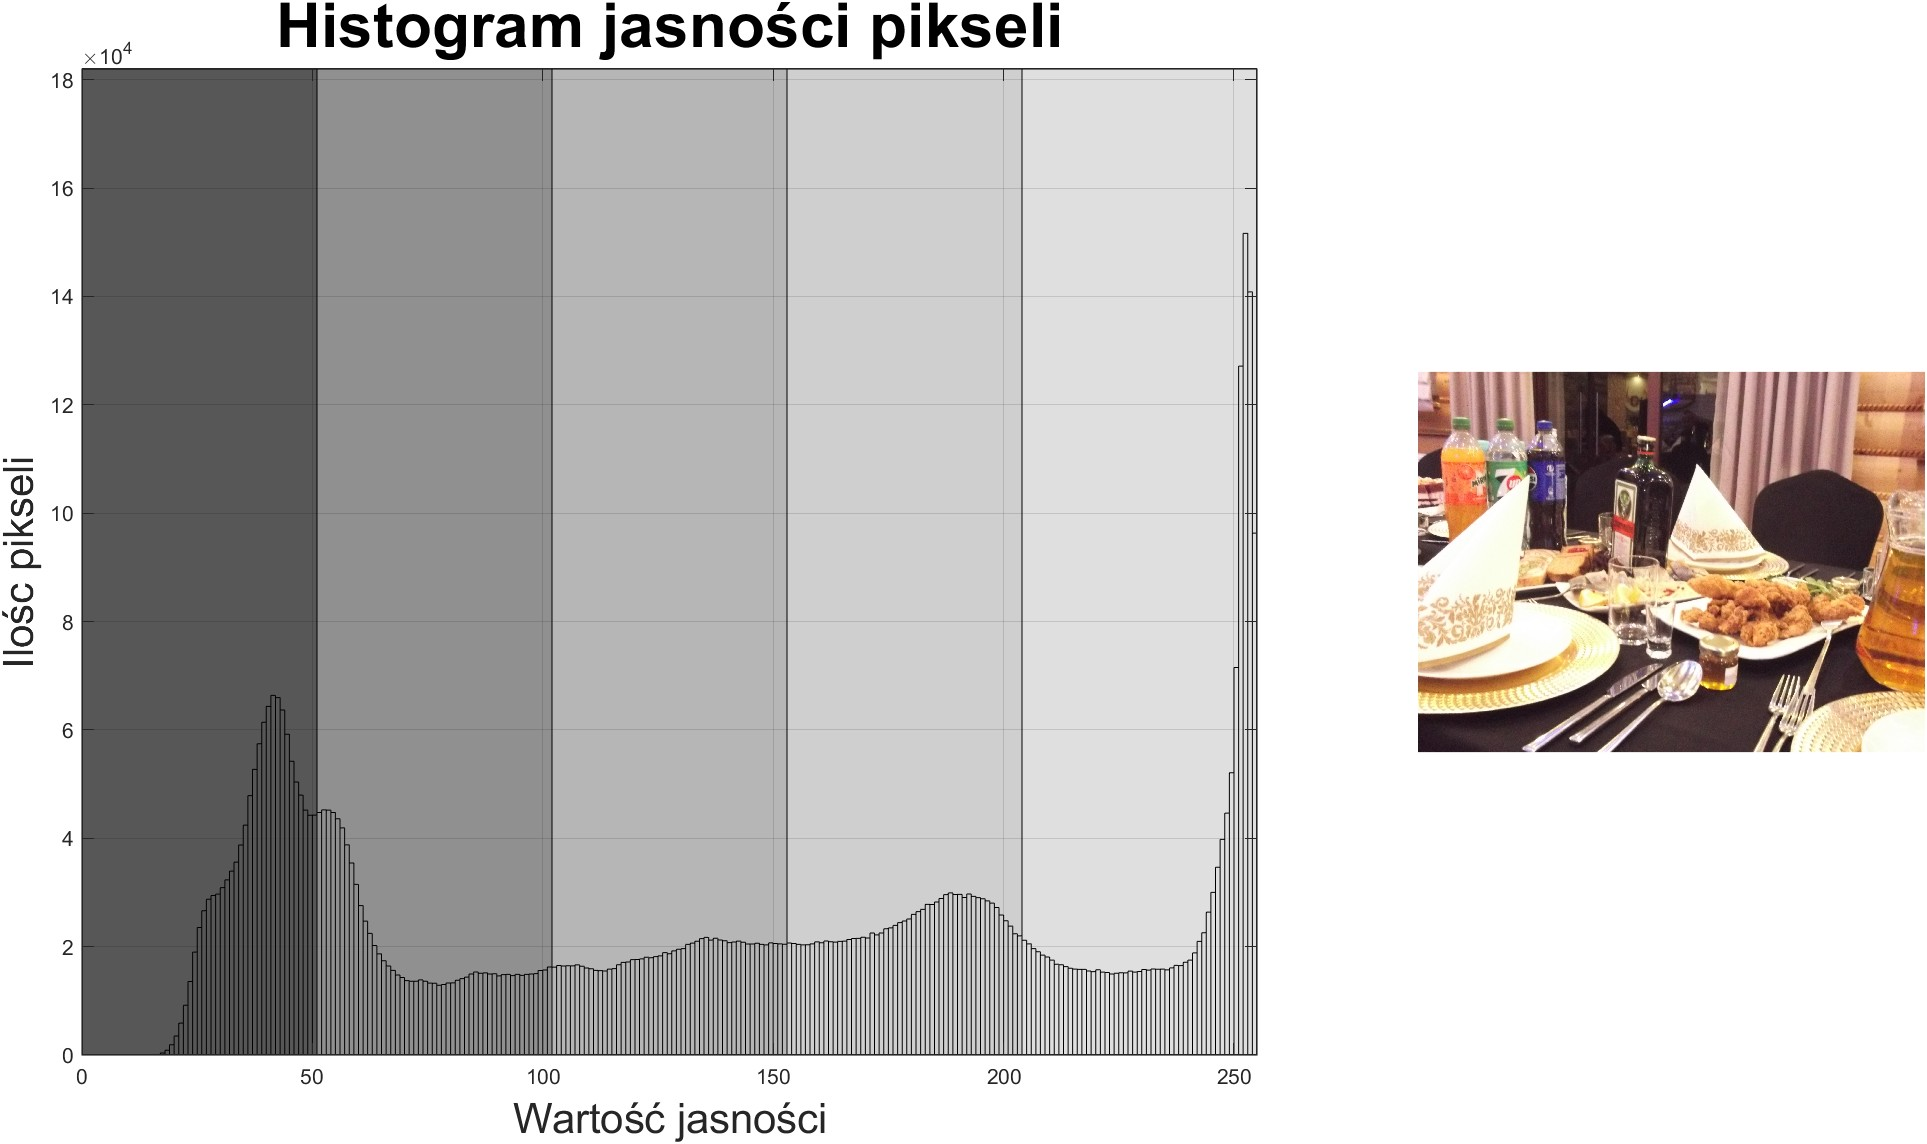
\includegraphics[width=\textwidth]{PTI_zdjęcia_i_histogramy/intensity/jagier3_intensity.jpg}



\newpage
\subsection{Barwa, odcień}
Hue -- z angielskiego coś pomiędzy barwą a odcieniem w fotografii odnosi się
do podstawowego koloru światła, czyli pozycji danego koloru w spektrum barw
widzialnych. Wyrażany jest w stopniach od $0$ do $360^o$ na kole
barw. Natomiast zmiana hue tylko przesuwa kolor, ale nie zmienia jego jasności
ani nasycenia. Nie badaliśmy wartości hue dla zebranych przez nas zdjęć analogowych,
ponieważ są czarno-białe. Analiza hue dla zdjęć cyfrowych pokazała nieznaczne różnice przy różnej ekspozycji.
\subsubsection{Kod}


\begin{verbatim}
    
    files = dir("photos\*.jpg");
    
    for i = 1:length(files)
    
    clear count g G im max n;
    im = imread(strcat("photos\", files(i).name));
    g = rgb2hsv(im);
    g = g(:,:,1);
    g = g*255;
    G = g(:);
    figure(1);
    set(gcf, 'Units', 'Normalized', 'OuterPosition', [0 0 1 1]); %wielkość okna
    subplot(1,3,[1,2]); 
    histogram(G,'FaceColor', '#ffffff');
    
    [count, n] = histcounts( G, 255 );
    max = max(count);
    max = max*1.2;
    
    xlim([0 255]);
    ylim([0,max]);
    
    grid on;
    title('Histogram odcienia pikseli','FontSize', 30);
    xlabel('Wartość odcienia','FontSize',20);
    ylabel('Ilośc pikseli','FontSize',20);
    
    subplot(1,3,3);
    imshow(im);
    
    exportgraphics(gcf, strcat("hue\", 
                        \\files(i).name(1:length(files(i).name)-4),"_hue.jpg"))
    close;
    
    end
    
  
    
    
    
    
    
    \end{verbatim}
\newpage


\subsubsection{Wyniki}
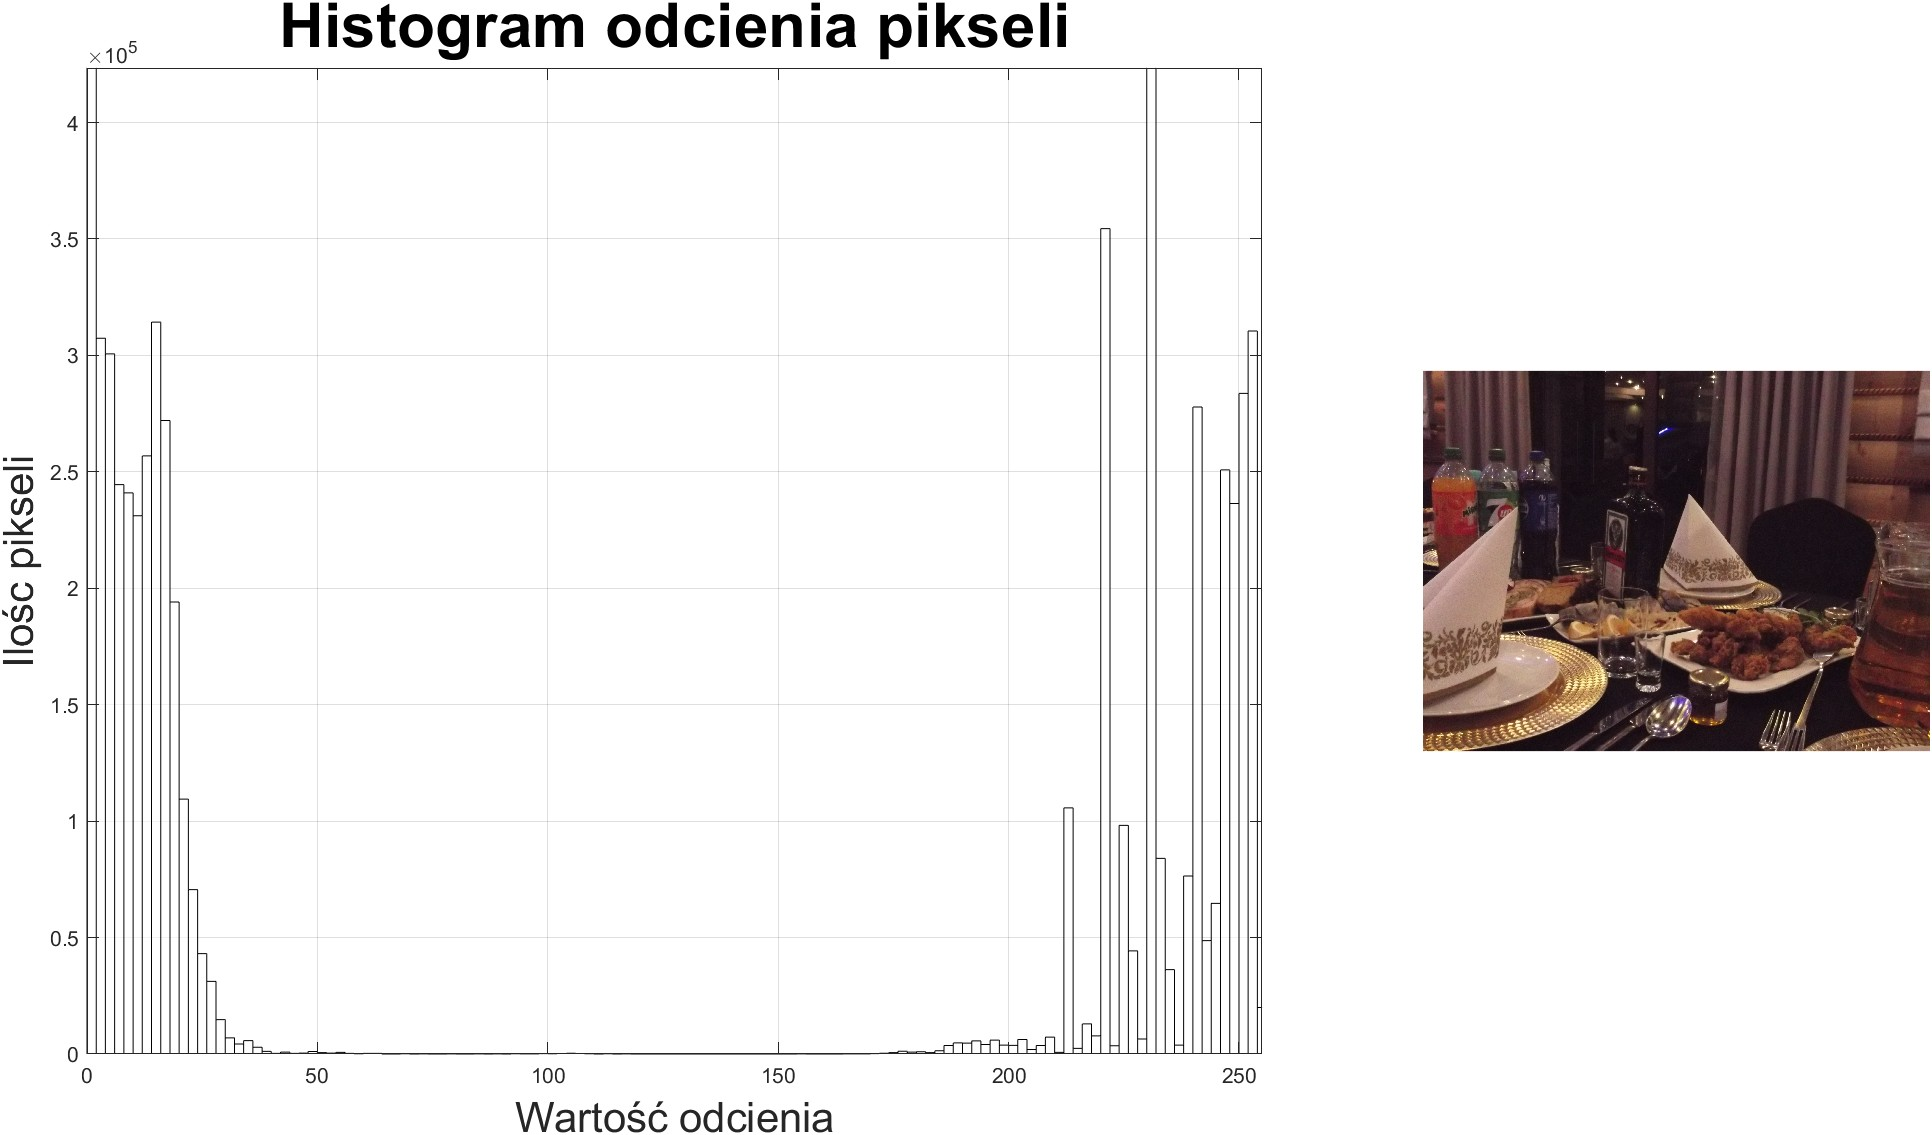
\includegraphics[width=\textwidth]{PTI_zdjęcia_i_histogramy/hue/jagier1_hue.jpg}
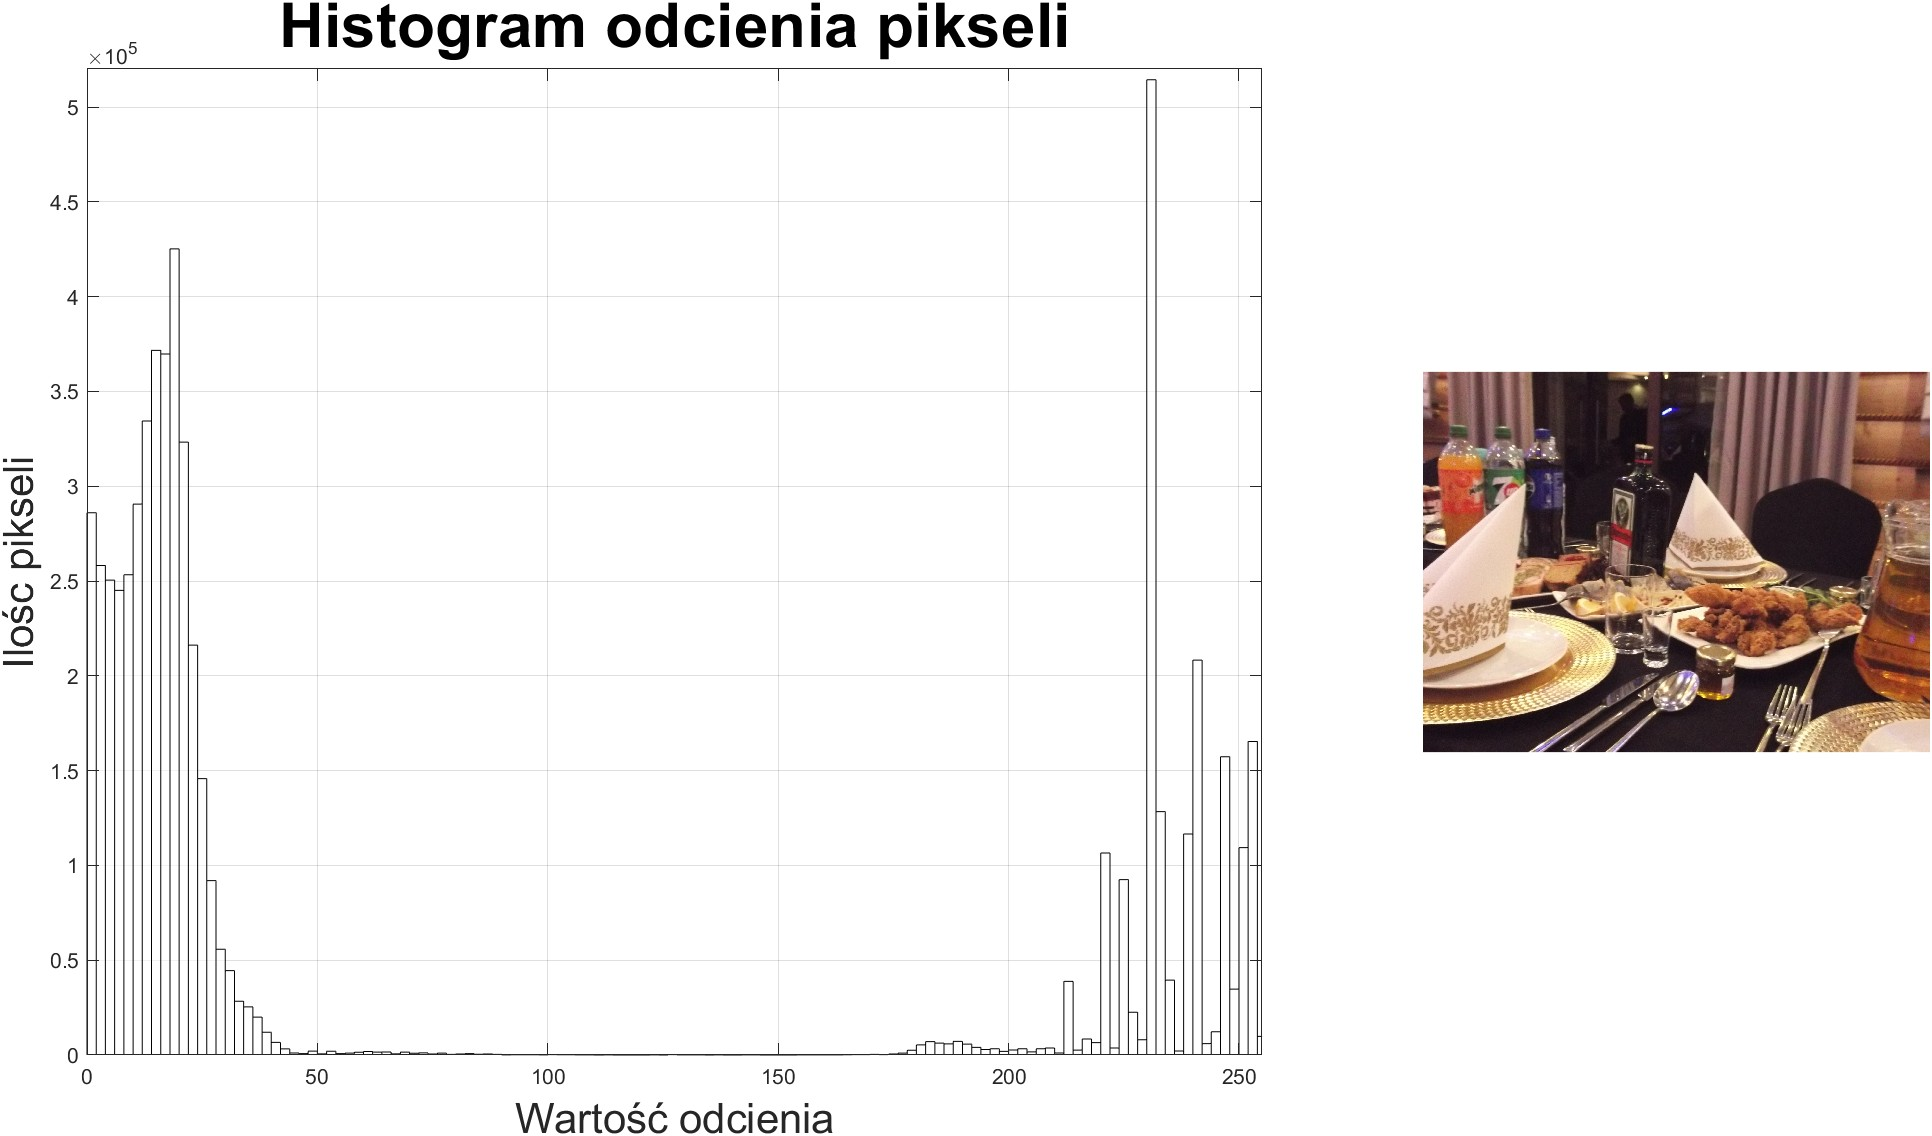
\includegraphics[width=\textwidth]{PTI_zdjęcia_i_histogramy/hue/jagier2_hue.jpg}
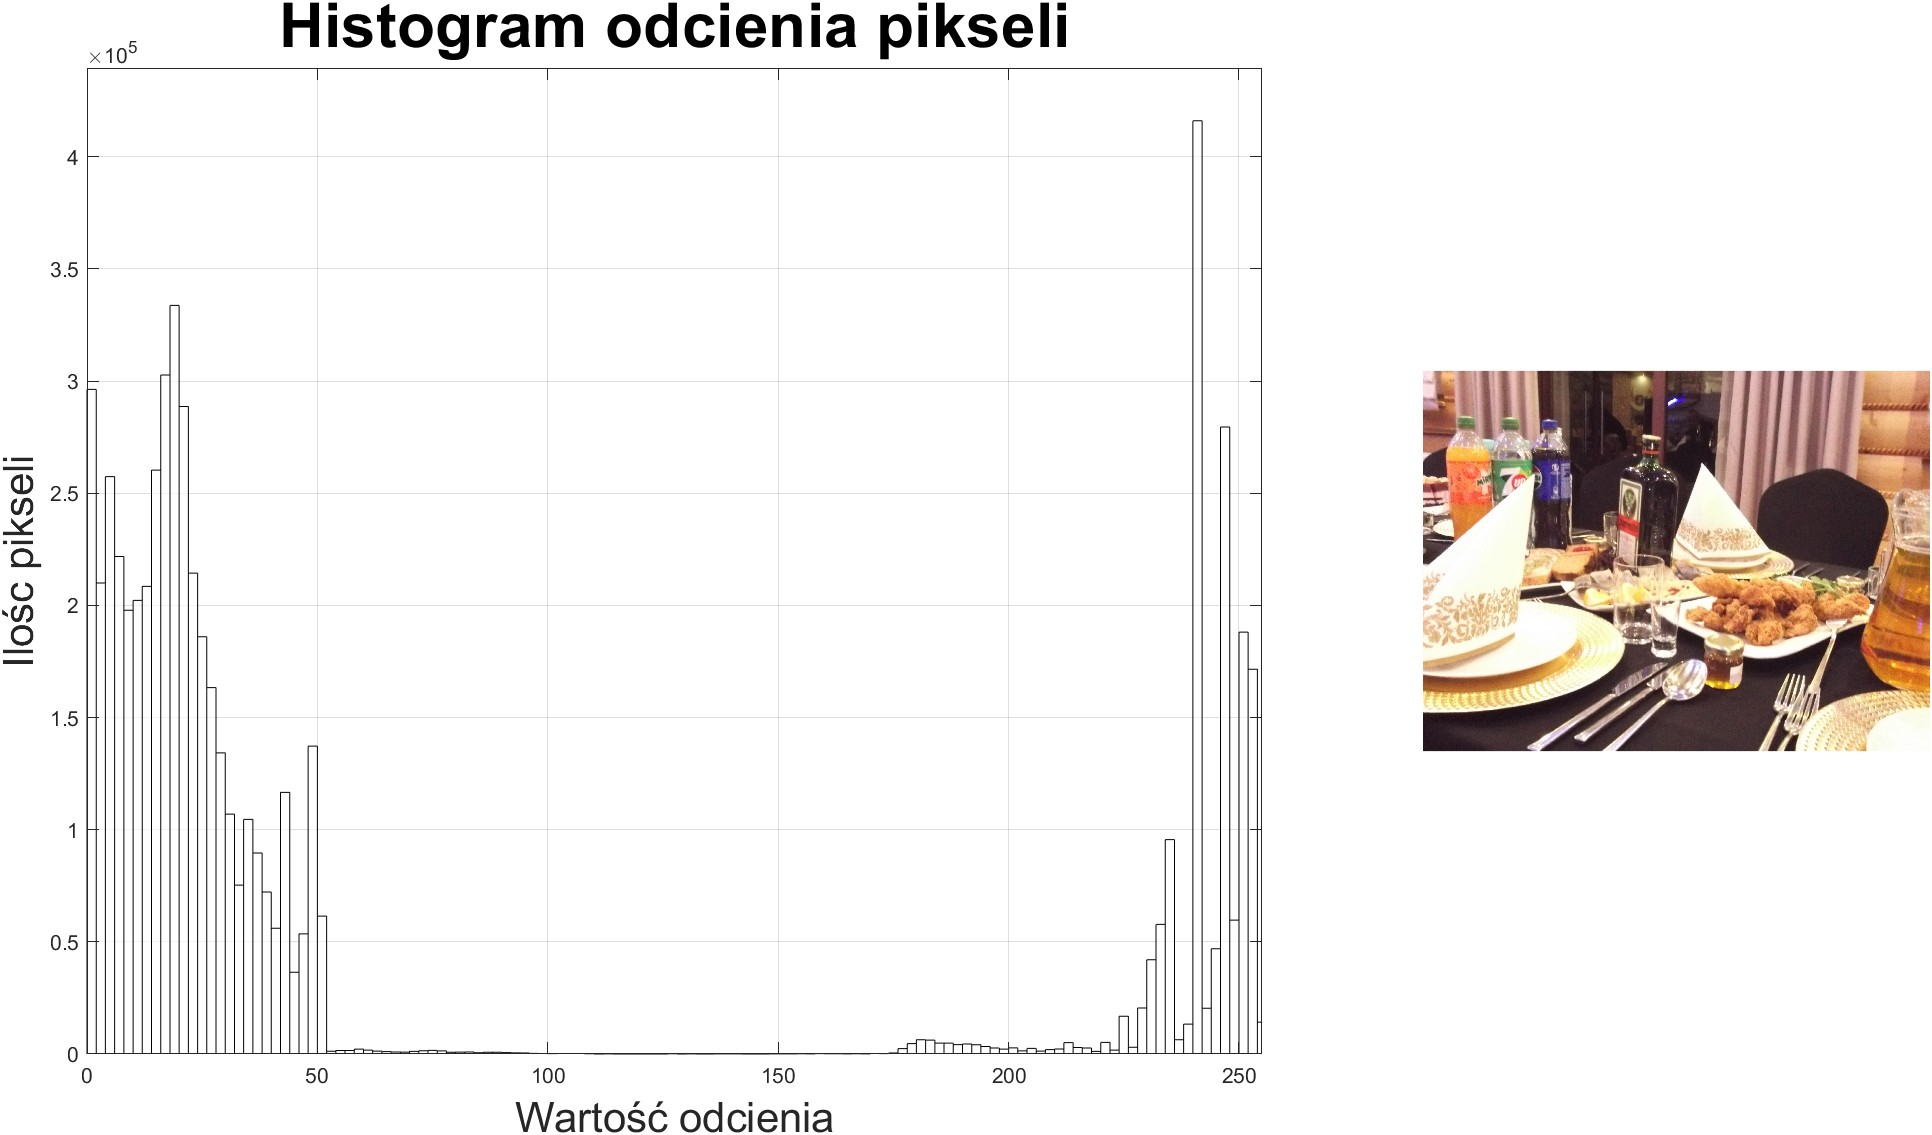
\includegraphics[width=\textwidth]{PTI_zdjęcia_i_histogramy/hue/jagier3_hue.jpg}



\newpage
\subsection{Saturacja}
Saturacja w fotografii to stopień intensywności kolorów na zdjęciu. Określa,
jak bardzo barwy są nasycone -- od wyblakłych i niemal czarno-białych (niska
saturacja) do bardzo żywych i intensywnych (wysoka saturacja). Tak samo jak z
hue nie badaliśmy saturacji dla zdjęć czarno-białych. Można zauważyć znaczne
różnice w saturacji zdjęć cyfrowych w zależności od stopnia naświetlenia.

\subsubsection{Kod}
\begin{verbatim}
files = dir("photos\*.jpg");

for i = 1:length(files)

clear count g G im max n;
im = imread(strcat("photos\", files(i).name));
g = rgb2hsv(im);
g = g(:,:,2);
g = g*255;
G = g(:);
figure(1);
set(gcf, 'Units', 'Normalized', 'OuterPosition', [0 0 1 1]); %wielkość okna
subplot(1,3,[1,2]); 
histogram(G,'FaceColor', '#ffffff');

[count, n] = histcounts( G, 255 );
max = max(count);
max = max*1.2;

xlim([0 255]);
ylim([0,max]);

grid on;
title('Histogram nasycenia pikseli','FontSize', 30);
xlabel('Wartość nasycenia','FontSize',20);
ylabel('Ilośc pikseli','FontSize',20);

subplot(1,3,3);
imshow(im);

exportgraphics(gcf, strcat("saturation\", 
            \\files(i).name(1:length(files(i).name)-4),"_saturation.jpg"))
close;

end

\end{verbatim}

\newpage
\subsubsection{Wyniki}

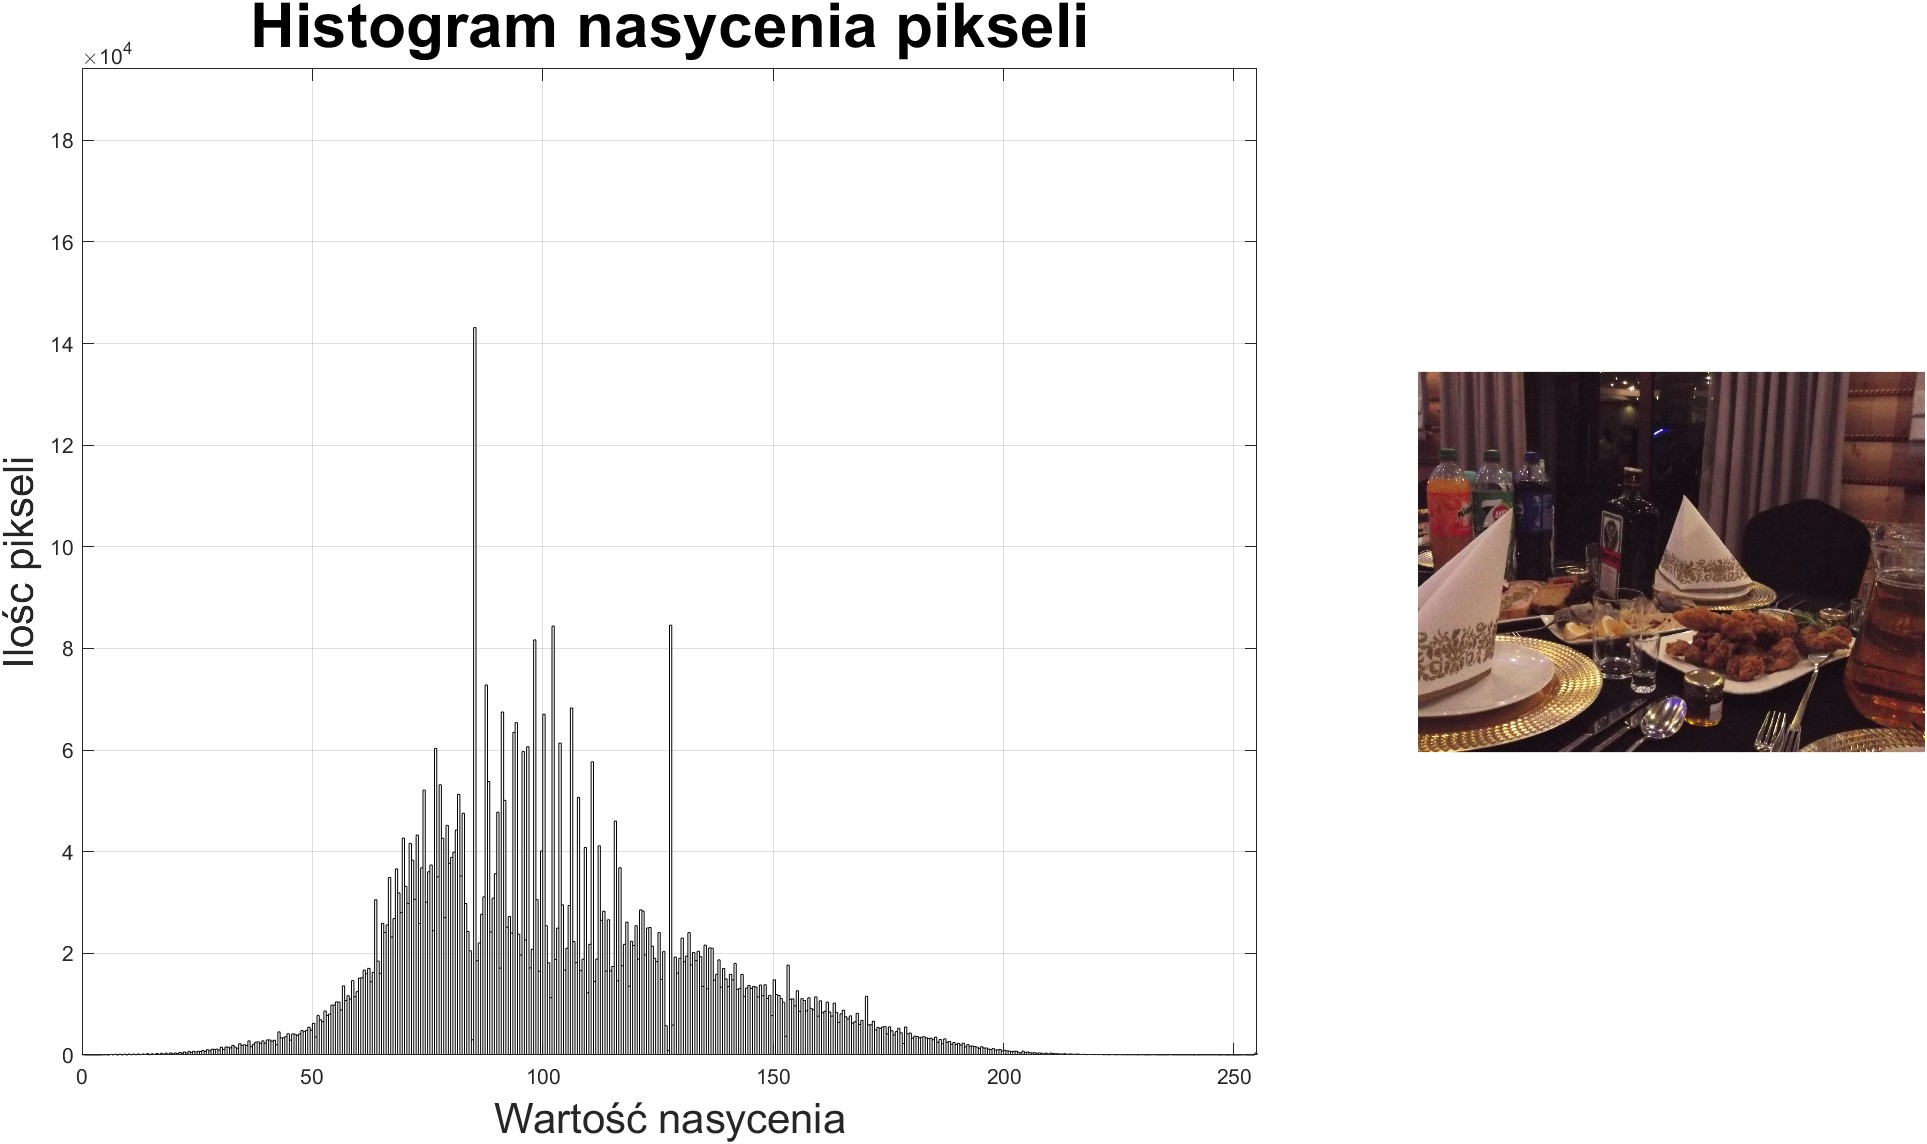
\includegraphics[width=\textwidth]{PTI_zdjęcia_i_histogramy/saturation/jagier1_saturation.jpg}
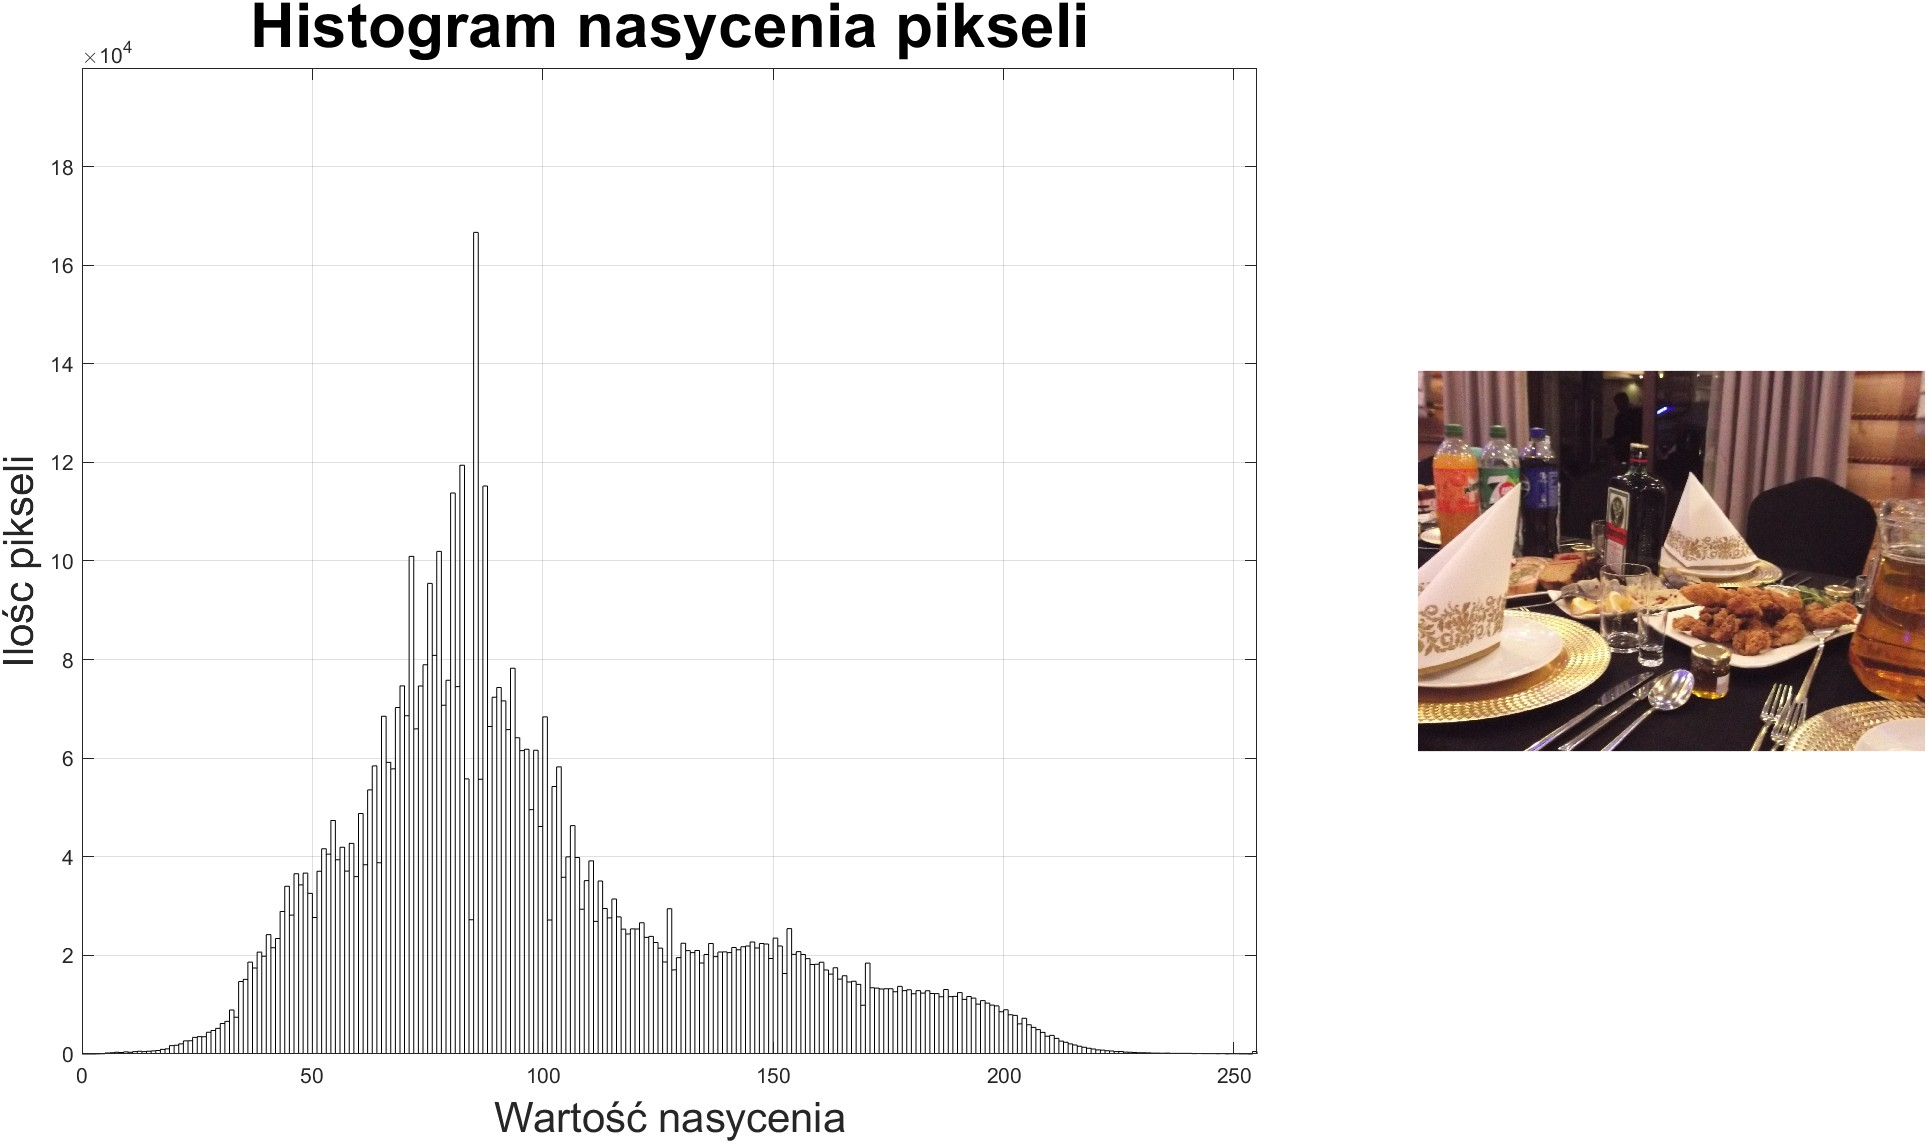
\includegraphics[width=\textwidth]{PTI_zdjęcia_i_histogramy/saturation/jagier2_saturation.jpg}
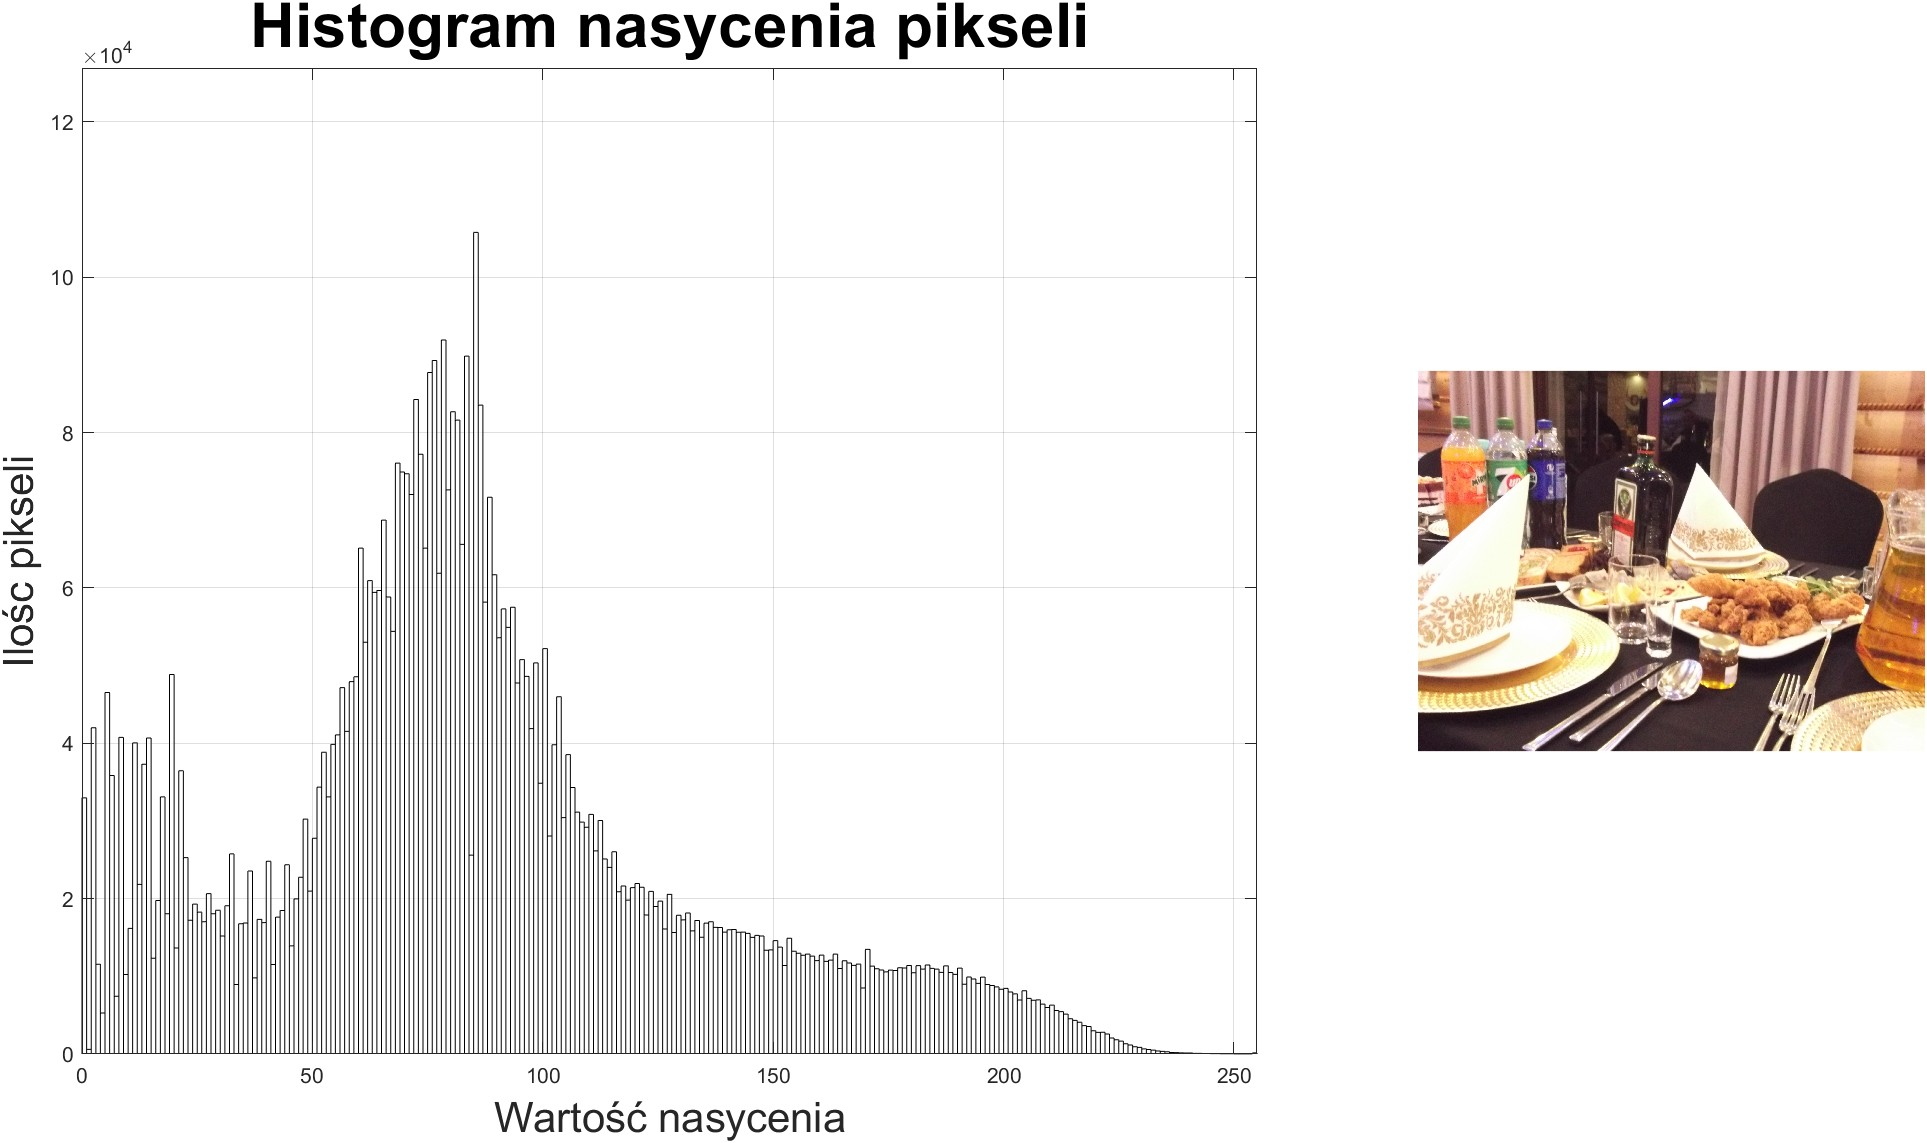
\includegraphics[width=\textwidth]{PTI_zdjęcia_i_histogramy/saturation/jagier3_saturation.jpg}

\newpage



\newpage
\subsection{Kontrast}
Kontrast w fotografii to różnica między jasnymi i ciemnymi obszarami zdjęcia.
Określa, jak bardzo elementy obrazu różnią się od siebie pod względem
jasności, koloru lub tonu. Wyższy kontrast sprawia, że zdjęcie wygląda
bardziej dynamicznie, a niski kontrast daje bardziej miękki, wyblakły
efekt.

\subsubsection{Kod}
\begin{verbatim}
    files = dir("photos\*.jpg");
cont = struct('plik', cell(1,length(files)), 'kontrast',
                \\cell(1,length(files)), 'jasnosc', cell(1,length(files)));

for i = 1:length(files)

clear g G l im j k m n R;
im = imread(strcat("photos\", files(i).name)); 
g = rgb2gray(im);
g = single(g);
g=g/255;
G = g(:);
I = mean(G);
[n, m] = size(g);
R =0.0;

for k=1:1:n
    for j = 1:1:m
        R = R + (g(k,j) - I)^2;
    end
end

R = R/(m*n);

R = sqrt(R);

%disp(["Kontrast zdjęcia" R]);
%disp(["Średnia jasność zdjęcia" I]);

cont(i).plik = files(i).name;
cont(i).kontrast = R;
cont(i).jasnosc = I;

end

writetable(struct2table(cont), 'contrast.csv')

\end{verbatim}
\subsubsection{Wyniki}
Co w przypadku naszego zdjęcia dało wyniki następujące:

\begin{table}[h]
    \centering
    \begin{tabular}{|c|c|c|}
        \hline
        Zdjęcie                      & Kontrast  & Jasność    \\ \hline
        Zdjęcie stołu niedoświetlone & 0.1856783 & 0.2637069  \\ \hline
        Zdjęcie stołu idealne        & 0.2608515 & 0.39802570 \\ \hline
        Zdjęcie stołu prześwietlone  & 0.3019148 & 0.54119000 \\ \hline
    \end{tabular}
    \caption{Wyniki dla używanego w raporcie przykładowego zdjęcia stołu}
\end{table}

\newpage
\subsection{Wnioski i plany na przyszłość}
Analiza danych zebranych w powyższych częściach okazała się trudnym zadaniem,
dlatego wrócimy do niej w kolejnym raporcie. Zamieszczamy jednak poniższą tablę,
której poprawności statystycznej dla ogółu danych nie jesteśmy pewni. Na podstawie
danych jesteśmy wciąż w stanie postawić hipotezę, że: im większe doświetlenie tym
wyższy kontrast i jasność. nirzsze


\begin{table}[h]
    \centering
    \begin{tabular}{|c|c|c|c|c|c|}
        \hline
        EV       & -1    & $+\delta$ & 0     & $+\delta$ & +1    \\ \hline
        Kontrast & 0.119 & +37 \%    & 0.163 & +26 \%    & 0.206 \\ \hline
        Jasność  & 0.231 & +27 \%    & 0.294 & +20 \%    & 0.352 \\ \hline
    \end{tabular}
    \caption{Średnie jasności i kontrastu od korekty naświetlenia}

\end{table}




\section{Wykorzystywane narzędzia}
W tej części naszego projektu korzystaliśmy z następujących narzędzi:
\begin{itemize}
    \item Programu Matlab -- do analizy zdjęć;
    \item Programu LibreOffice Calc -- do analizy wyników ankiety;
    \item $\LaTeXe{}$ -- do przygotowania raportu;
    \item Google Drive -- do udostępniania plików;
    \item 7zip -- do kompresji zdjęć;
    \item Aparatów:
          \begin{itemize}
              \item Canon EOS 300 z obiektywem Tamron 28-105mm 1:4-5.6 i kliszą Fomapan 400
              \item Fujifilm FinePix L55 Digital Camera -- Black (12MP, 3x Optical Zoom)
          \end{itemize}
\end{itemize}


\section{Podział obowiązków}
Po wyborze celu projektu wszyscy zajęliśmy się zdobywaniem wiedzy na
temat problemów fotografii analogowej, a także możliwych poprawy jakości zdjęć.\newline


Posiadając wstępną wiedzę na temat materii projektu organicznie wstępnie
podzieliliśmy się zajęciami zgodnie z naszymi zainteresowaniami: \newline
\begin{itemize}
    \item pozyskiwanie materiałów testowych -- Aleksandra Wójcik, Bartosz Wójcik;
    \item opracowanie skryptów do analizy zdjęć i zbieranie informacji do algorytmu -- Katarzyna Szwed, Karol Sęk, Michał Juszkiewicz;
    \item opracowywanie raportu -- Patrycja Szałajko, Natalia Szymańska, Filip Sajko.
\end{itemize}







\end{document}